\documentclass[titlepage, 12pt]{article}
%----------------------------Preamble-------------------------------%
%---------------------------Packages----------------------------%
\usepackage{geometry}
\geometry{a4paper, margin = 1.0in} 
\usepackage{graphicx, float}            % Graphics/Images.
\graphicspath{{figs/}}                  % Path to Image Folder.
\usepackage{natbib}                     % For bibliographies.
\bibliographystyle{agsm}                % Bibliography style.
\usepackage[english]{babel}             % Language typesetting.
\usepackage[dvipsnames]{xcolor}         % Color names.
\usepackage{listings, lstlinebgrd}      % Verbatim-Like Tools.
\usepackage{mathtools, amssymb}         % amsmath and symbols.
\usepackage{multicol, enumitem}         % Multi-column/enumerate.
\usepackage{hyperref}                   % Allows for hyperlinks.
\hypersetup{
    colorlinks=true,
    linkcolor=blue,
    filecolor=magenta,
    urlcolor=Cerulean,
    citecolor=SkyBlue
}                                       % Colors for hyperref.
\usepackage[
    font={scriptsize},
    hypcap=true,
    labelsep=colon
]{caption}                              % Figure captions.
\usepackage[%
    font=scriptsize,
    labelformat=simple,
    labelsep=colon%
]{subcaption}                           % Subfigure captions.
\usepackage[
    toc,
    acronym,
    nogroupskip
]{glossaries}                           %Glossaries and acronyms.
%------------------------New Commands---------------------------%
\newcommand*\diff{\mathop{}\!\mathrm{d}}
\renewcommand*{\glstextformat}[1]{\textcolor{RoyalBlue}{#1}}
\renewcommand{\glsnamefont}[1]{\textbf{#1}}
\renewcommand\labelitemii{$\circ$}
\renewcommand\thesubfigure{%
    \arabic{figure}.\arabic{subfigure}%
}
\addto\captionsenglish{\renewcommand{\figurename}{Fig.}}
\newglossarystyle{longpara}{%
    \setglossarystyle{long}%
    \renewenvironment{theglossary}{%
        \begin{longtable}[l]{@{}p{\hsize}@{}}
    }{\end{longtable}}%
    \renewcommand{\glossentry}[2]{%
        \glstarget{##1}{\glossentryname{##1}}%
        \tabularnewline%
        \glossentrydesc{##1}{.~##2}
        \tabularnewline%
        \tabularnewline
    }%
}
%--------------------------LENGTHS------------------------------%
% Spacing for multi-column and enumerate environments.
\setlength{\multicolsep}{6pt}
\setlist[enumerate]{itemsep=0pt,topsep=3pt}

% Indent and paragraph spacing.
\setlength{\parindent}{0em}
\setlength{\parskip}{0em}
%----------------------------GLOSSARY-------------------------------%
\makeglossaries
\loadglsentries{glossary}
\loadglsentries{acronym}
%---------------------------Title Page------------------------------%
\begin{document}
    \title{{\Huge{rss\_ringoccs: User Guide}\\}V1.2}
    \author{\copyright
            Team Cassini at Wellesley College\\
            Richard G. French$\overset{^*}{,}$
            Sophia R. Flury,
            Jolene W. Fong,\\
            Ryan J. Maguire, and
            Glenn J. Steranka}
    \date{%
        $^*$\textit{%
            \small{Cassini Radio Science Team Leader, \\
            rfrench@wellesley.edu}
        }\\[4ex]%
        \today%
    }
    \pagenumbering{roman}
    \maketitle
    \newpage
    \tableofcontents
    \newpage
    \listoffigures
    \listoftables
    \clearpage
    \pagenumbering{arabic}
    \section{Introduction}
        The Cassini \gls{rss} was used during the Cassini
        orbital tour of Saturn to observe a superb series
        of ring occultations that resulted in high-resolution,
        high-SNR radial profiles of Saturn's rings at three
        radio wavelengths: 13 cm (S band), 3.6 cm (X band),
        and 0.9 cm (Ka band). Radial optical depth profiles of
        the rings at 1- and 10-km resolution produced by
        Essam Marouf of the Cassini RSS team,
        using state-of-the-art signal processing techniques
        to remove diffraction effects, are available on the
        \gls{nasa} \gls{pds}.%
        \footnote{\url{https://pds-rings.seti.org/cassini/rss/index.html}}
        These archived products are likely to be quite adequate
        for many ring scientists, but for those who wish
        to generate their own diffraction-reconstructed ring
        profiles from Cassini RSS observations, we provide
        \texttt{rss\_ringoccs}: a suite of Python-based analysis
        tools for radio occultations of planetary rings.%
        \footnote{%
            \texttt{rss\_ringoccs} may be found from
            \url{https://github.com/NASA-Planetary-Science/rss\_ringoccs}
        }
        \par\hfill\par
        The purpose of \texttt{rss\_ringoccs} is to enable
        scientists to produce ``on demand'' radial optical
        depth profiles of Saturn's rings from the raw RSS data,
        without requiring deep familiarity
        with the complex processing steps involved in calibrating
        the data and accounting for the effects of diffraction.
        The code and algorithms are extensively documented,
        providing a starting point
        for users who wish to test, refine, or optimize the
        straightforward methods we have employed.
        Our emphasis has been on clarity, sometimes at the
        expense of programming efficiency and execution time.
        \texttt{rss\_ringoccs} does an excellent job
        of reproducing existing RSS processed ring occultation
        data already present on NASA's PDS Ring-Moon Systems
        Node -- detailed comparisons of representative examples of
        our results with those on the PDS are presented below in
        Section~\ref{sec:pds_valid}.
        However, we make no claim to having achieved the
        state-of-the-art in every respect. 
        In a project this complex, bugs may well be present,
        and we encourage users to report any errors,
        augment our algorithms, and share these improvements
        so that they can be incorporated in future editions of
        \texttt{rss\_ringoccs}.
        \par\hfill\par
        This document provides an introduction to RSS ring
        occultations, directs users to required and recommended
        reading, describes in detail how to set up
        \texttt{rss\_ringoccs}, and explains how to
        obtain RSS data files and auxiliary files required
        by the software. It provides an overview of the
        processing pipeline, from raw data to final
        high-resolution radial profiles of the rings, and
        guides users through a series of simple examples to
        illustrate the use of \texttt{rss\_ringoccs}.
        The algorithms and code are validated by comparison
        with Voyager and Saturn RSS results on the PDS archive,
        and with analytical results. Finally, it includes
        practical considerations for users, and benchmarks
        of program execution time.
        \subsection{Getting help}
            \texttt{rss\_ringoccs}\ is easy to
            install and use, but if you have questions
            along the way please don't hesitate
            to get in touch with us. We recommend
            that you post an issue to the \texttt{rss\_ringoccs}
            repository%
            \footnote{\url{https://github.com/NASA-Planetary-Science/%
                      rss\_ringoccs/issues}}
            so that other users can join in
            the conversation, but you are also
            free to contact the lead author of the project, Richard G. French, at
            \textit{rfrench@wellesley.edu}. 
            For reference, we provide detailed documentation of
            the software online at
            \url{https://rss-ringoccs.readthedocs.io/en/master/}.
        \subsection{What is an RSS ring occultation?}
            In its simplest form, an RSS ring occultation occurs when a radio
            signal transmitted from a spacecraft's \gls{hga} passes
            through the rings on the way to a
            \gls{dsn} receiving antenna
            on Earth. The received signal at Earth is affected by
            interactions of the radio signal with the swarm of ring
            particles, including attenuation, scattering,
            Doppler-shifting of the signal,
            and diffraction. We refer to
            the process of compensating for diffraction to obtain the
            intrinsic radial optical depth profile of the rings as
            \gls{diffraction reconstruction}
            or \gls{fresnel inversion},
            since the reconstruction process is based
            on the mathematical principles of Fresnel optics. 
        \subsection{Overview of Cassini RSS ring observations}
            Over the course of the Cassini orbital tour of Saturn,
            the geometry of RSS ring occultations varied due to
            changes in the orbiter's trajectory and in
            the aspect of the rings as seen from Earth
            during Saturn's orbit around the
            Sun. The opening angle of Saturn's rings
            as a function of time as seen from Earth
            is shown below in \textbf{Fig.~\ref{fig:Bdeg}}.
            \begin{figure}[H]
                \centering
                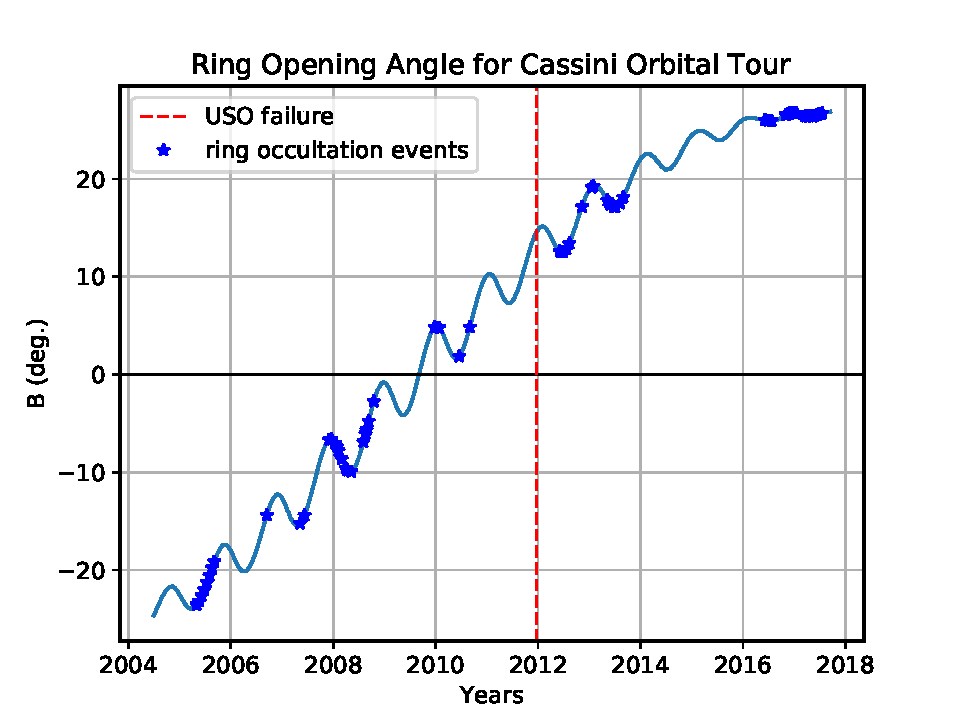
\includegraphics[width=0.8\textwidth]
                    {poster_B_plot_20180907}
                \caption[Ring opening angle vs. year]{%
                    Ring Opening angle $(B)$ vs. Time.
                    The rings are edge-one for an opening angle of
                    $B=0$.
                    In 2012, the on-board ultra-stable oscillator (USO)
                    failed, complicating diffraction reconstruction
                    thereafter. Symbols mark the time and ring opening angle for 
                    individual Cassini RSS ring observations.
                }
                \label{fig:Bdeg}
            \end{figure}
            Individual occultations are identified by the Cassini
            \gls{rev number} $n$, corresponding roughly to the
            $n^{\rm th}$ orbit of Cassini around Saturn, during
            which the occultation occurred. During the
            \gls{ingress} portion of an occultation, the orbital
            radius of the intercept point in the ring plane of
            the incident ray from the spacecraft decreases with
            time; the radius increases with time during the
            \gls{egress} portion of an occultation. During a
            \gls{diametric occultation}, the ingress and egress
            portions of the occultation are interrupted by
            passage of the spacecraft behind the planet itself as
            seen from Earth, resulting in an
            \gls{atmospheric occultation}. For the Grand Finale orbits 
            of the Cassini mission, the spacecraft trajectory was changed, resulting 
            in periapse being between the rings and Saturn. On these orbits, there were up to 
            three separate ring occultations: a rapid egress `proximal' occultation when the
            spacecraft was in front of the planet as viewed from Earth, followed by a more
            traditional chord occultation with an ingress and egress part, as the spacecraft receded from Earth behind the rings.
            The view from Earth of the ingress and egress portions of
            a diametric occultation on Rev 7 is shown in
            \textbf{Fig.~\subref{fig:rev7}}.
            During a \gls{chord occultation},
            the ingress and egress occultations are contiguous.
            The Earth view of the chord occultation
            on Rev 54 is shown in \textbf{Fig.~\subref{fig:rev54}}.
            \begin{figure}[H]
                \centering
                \begin{subfigure}[b]{0.48\textwidth}
                    \centering
                    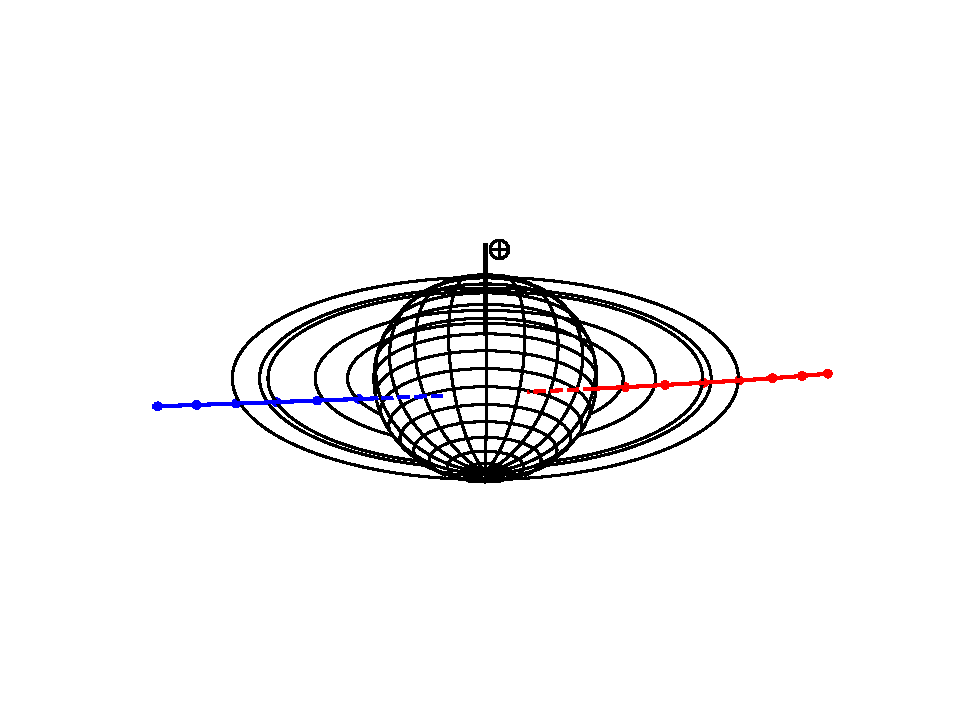
\includegraphics[%
                        trim={0.0in 1.0in 0.0in 1.0in},
                        clip,
                        width=\textwidth
                    ]{figs/rev7_earthview_UG.pdf}
                    \subcaption{Rev007}
                    \label{fig:rev7}
                \end{subfigure}
                \begin{subfigure}[b]{0.48\textwidth}
                    \centering
                    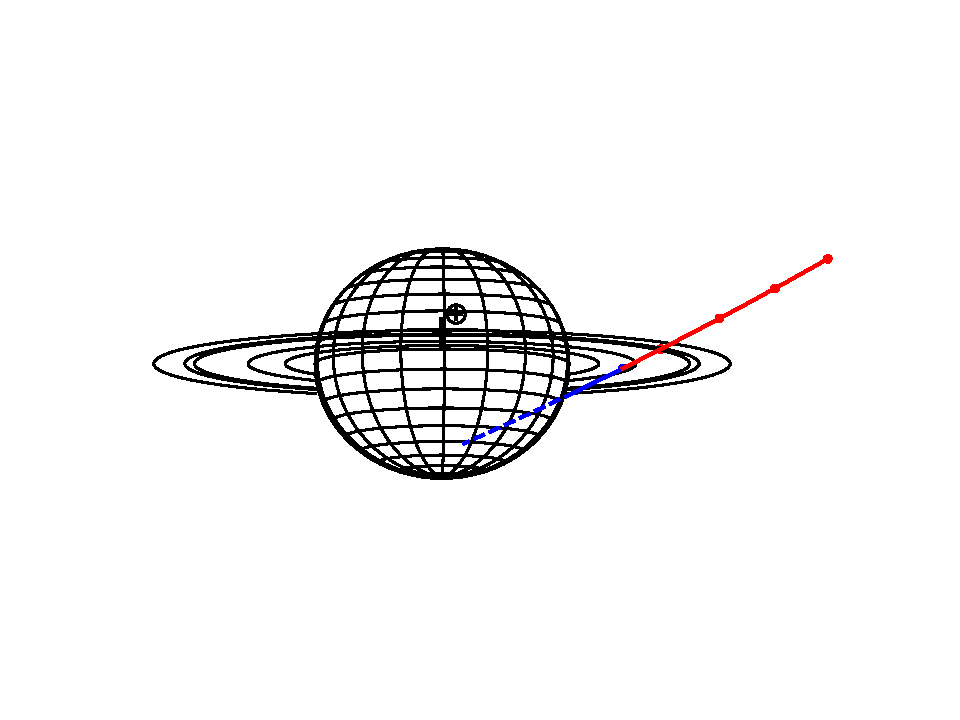
\includegraphics[%
                        trim = {0.0in 1.0in 0.0in 1.0in},
                        clip,
                        width=\textwidth
                    ]{figs/rev54_earthview_UG.pdf}
                    \subcaption{Rev054}
                    \label{fig:rev54}
                \end{subfigure}
                \caption[Earth View of Cassini During Rev007 and Rev054]{%
                    Earth view of Cassini during the Rev007
                    and Rev054 ring occultation observations.
                    The red solid lines represent the ingress portion of
                    an occultation and the blue solid lines represent the
                    egress portion. The blue and red dashed lines are the
                    part of the occultation that is blocked by Saturn.
                }
            \end{figure}
        \subsection{Cassini RSS ring occultation
                    observations on NASA's PDS}
            There are two categories of Cassini RSS observations
            on the PDS: raw data  in \gls{rsr} files
            that contain the digitized spacecraft signal
            as received at the DSN, and higher-level products
            (reduced data) that have been processed by
            the RSS team, including diffraction-reconstructed
            radial profiles of the optical depth of
            Saturn's rings and associated geometric and
            calibration information.
            \texttt{rss\_ringoccs} processes raw
            RSR files and independently produces
            higher-level products that can be saved as
            files similar in form and content to those
            already on the PDS, but with a user-defined
            radial resolution.
            \subsubsection{Raw RSS data files}
                \label{sec:rawRSSfiles}
                The raw data  produced by the DSN that contain
                the original observations of all Cassini
                occultation observations are recorded in
                RSR files, described in more detail in the
                \textit{Cassini Radio Science Users Guide}
                (Section~\ref{sec:CRSUG}).
                During Cassini RSS occultations,
                RSR files were typically recorded at two
                bandwidths: 1 kHz and 16 kHz -- both types are available on the PDS for nearly all Cassini RSS ring experiments.
                The \texttt{rss\_ringoccs}
                package can handle either version
                and they give nearly identical results,
                although the processing time for the
                16 kHz files is significantly longer.
                We provide convenient scripts in
                \texttt{rss\_ringoccs}
                (Section~\ref{sec:getRSR})
                to download both 1 kHz and 16 kHz RSR files before USO failure
                from the PDS archive. The 1 kHz files are preferred for nearly all
                cases; the 16 kHz files are required in cases where very high spatial
                resolution is desired.
            \subsubsection{Higher-level products}
                Essam Marouf of the Cassini RSS science
                team has produced a comprehensive set of
                set of higher-level products for
                ring occultation observations, available at
                \url{https://pds-rings.seti.org/viewmaster/volumes/CORSS_8xxx/CORSS_8001}.
                This archive set contains 1- and 10-km resolution
                diffraction-reconstructed profiles
                from S-, X- and Ka-band observations
                of Revs 7 through 137. \textit{Users interested in low-resolution ($\simeq 10$ km)
                ring profiles are advised to use the existing PDS results, rather than to use \texttt{rss\_ringoccs} to produce them, since our software package does not implement the low-pass filtering techniques used for the PDS results to obtain the 10 km resolution profiles.}
                 \par\hfill\par
            \subsection{Required and recommended reading}
            With this overview of RSS ring occultation
            observations and data in hand,
            we strongly recommend that all users
            familiarize themselves with several key
            documents before using the \texttt{rss\_ringoccs}
            package. Our internal documentation of the
            \texttt{rss\_ringoccs} code makes frequent
            reference to the following two documents:
            \subsubsection{Cassini Radio Science User's Guide}
                \label{sec:CRSUG}
                The most complete practical introduction
                to Cassini RSS ring observations is contained
                in the \textit{Cassini Radio Science User's Guide}%
                \footnote{Available from
                          \url{https://pds-rings.seti.org/cassini/rss/}}
                \citep{CRSUG2018}.
                We regard this as \textit{required reading}.
                Chapter 2
                describes the \textit{open-loop}
                \gls{rsr} files that
                contain the raw RSS ring occultation data,
                and Chapter
                3.3 summarizes the analysis steps to produce a
                diffraction reconstruction ring optical depth
                profile from the observations.
                \textit{For the remainder of this guide, we
                        will assume that all readers have familiarized
                        themselves with this material.}
            \subsubsection{Marouf, Tyler, and Rosen (1986) - MTR86}
                The definitive reference for
                diffraction reconstruction of
                RSS occultations is \citealt{Marouf1986}:
                Marouf, Tyler and
                Rosen's classic ``Profiling Saturn's rings by radio
                occultation.''
                We refer to this as MTR86.
                For copyright reasons,
                we cannot include MTR86 in this
                GitHub repository, but we highly recommend that
                scientists making use of radio occultation data
                have this paper readily at hand. It
                documents the Fresnel inversion method of
                diffraction reconstruction,
                complete with application to Voyager
                RSS occultation observations of Saturn's rings.
                This is \textit{recommended reading} for beginning users
                of \texttt{rss\_ringoccs}, and \textit{required reading}
                for anyone wishing to understand the
                inner workings of the \texttt{rss\_ringoccs}
                software package.
            \subsubsection{Online Documentation}
            Online documentation of \texttt{rss\_ringoccs} functions, scripts, and modules can be found at \url{https://rss-ringoccs.readthedocs.io/en/master/}.
            \subsubsection{For more information...}
                Readers interested in an overview of Cassini RSS
                instrumentation and science goals are encouraged
                to read ``Cassini Radio Science'' by
                \citealt{Kliore2004}.
                Scientific results making use of
                Cassini RSS occultation observations include
                \citealp{Colwell2009},
                \citealp{ElMoutamid2016},
                \citealp{French2016a},
                \citealp{French2016b},
                \citealp{French2017}
                \citealp{Marouf2011},
                \citealp{Nicholson2014a},
                \citealp{Nicholson2014b},
                \citealp{Rappaport2009},
                and
                \citealp{Thomson2007}.
    \section{Setting things up}
        This section provides step-by-step
        instructions for setting up the \texttt{rss\_ringoccs}
        package and associated data files. We assume
        that all users are familiar with basic unix commands
        and introductory-level Python.
        \subsection{System requirements}
            The \texttt{rss\_ringoccs} repository has been developed
            and tested on the following hardware,
            unix-based operating systems, and shells:
            \begin{table}[H]
                \centering
                \begin{tabular}{|l|l|l|l|}
                    \hline
                    Hardware&Operating System&Shell &GB of RAM\\
                    \hline
                    MacBookPro, iMac & MacOS 10.13.4, 10.14.5
                    &bash
                    &8, 16, and 32\\
                    Mac mini&Linux Ubuntu Budgie 16&bash&8\\
                    MacBookPro&Linux Ubuntu 16&bash&8\\
                    ThinkMate&Linux Debian&bash&32\\
                    \hline
                \end{tabular}
                \caption{Hardware and operating systems}
                \label{tab:OS}
            \end{table}
            We strongly recommend that users run
            \texttt{rss\_ringoccs}
            on a system with at least 16 GB of RAM
            (preferably 32 GB)
            to minimize disk-based memory swapping, which can
            significantly increase the run time when processing an
            entire occultation at high resolution.
        \subsection{Downloading the \texttt{rss\_ringoccs}
                    repository from GitHub}
                    
                    To download via \texttt{git clone}, open a terminal window and navigate to the directory below which you wish to install \texttt{rss\_ringoccs} and type the command:
                        % git clone installation
       
            \begin{lstlisting}[%
                language=bash,
                basicstyle=\footnotesize\ttfamily,
                frame=single,
                escapechar=",
                gobble=16,
                columns=fullflexible]
                git clone  https://github.com/NASA-Planetary-Science/rss_ringoccs.git
            \end{lstlisting}
            %Follow these steps to download and install
            \par
            To download \texttt{rss\_ringoccs} via ZIP file, visit\\ \url{https://github.com/%
                           NASA-Planetary-Science/rss_ringoccs}
                      and click on the green \textit{Clone or Download}
                      pull-down menu at the upper right and click on \textit{Download ZIP}. \texttt{rss\_ringoccs-master.zip} will appear in your local \texttt{Downloads} directory; unzip it and move it to your desired directory. Unzipping the file will create an \texttt{rss\_ringoccs-master} folder, as opposed to the \texttt{rss\_ringoccs} folder that appears when the repository is downloaded using \texttt{git clone}. 
                      \par
  


            
        \subsection{Install Python 3 and required packages}
            \texttt{rss\_ringoccs} has been developed under Python 3,
            in particular Python 3.5, 3.6, and 3.7.
            Our code has been tested under the following
            Python configurations:
            \begin{table}[H]
                \centering
                \begin{tabular}{|l|l|l|l|}
                    \hline
                    Operating System&Distribution&
                    Version&URL\\
                    \hline
                    MacOS 10.14.1&Anaconda&
                    3.6.3&\url{https://www.anaconda.com}\\
                    MacOS 10.14.2&Anaconda&
                    3.7.1&\url{https://www.anaconda.com}\\
                    MacOS 10.14.5&Anaconda&
                    3.6.8&\url{https://www.anaconda.com}\\
                    Linux Ubuntu Budgie 16&Anaconda&
                    3.6.3&\url{https://www.ubuntu.com}\\
                    Linux Ubuntu 18&Anaconda&3.6.3&
                    \url{https://www.ubuntu.com}\\
                    Linux Debian &Anaconda&
                    3.6.3&\url{https://www.debian.org}\\
                    \hline
                \end{tabular}
                \caption{Python versions compatible with
                         \texttt{rss\_ringoccs}}
                \label{tab:Python}
            \end{table}
            Once the  \texttt{rss\_ringoccs} package has been downloaded,
            the user will need to install Python 3 and
            various dependencies. The easiest way to do this by running
            the setup script
            \texttt{rss\_ringoccs\_config.sh},
            included in the download. This will install
            Python 3 using Anaconda, as well as all of the necessary
            packages, and update and source the \texttt{.bash\_profile} 
            and \texttt{.bashrc} files. For users who have already installed Python,
            this script will update \texttt{conda} and then check that
            \texttt{spiceypy} and other packages exist on the machine. To run the setup script, navigate to the \texttt{rss\_ringoccs} directory in a terminal and run the following:
            \begin{lstlisting}[%
                basicstyle=\small\ttfamily,
                columns=fullflexible,
                keepspaces=true,
                literate={~}{$\sim$}{1},
                frame=single,
                gobble=16
            ]
                ./rss_ringoccs_config.sh
            \end{lstlisting}
            The installation process will begin,
            and may take several minutes. By default, the Anaconda3 distribution should contain ipython, an enhanced interactive Python shell. If it is absent, type the following command:
                        \begin{lstlisting}[%
                basicstyle=\small\ttfamily,
                columns=fullflexible,
                keepspaces=true,
                literate={~}{$\sim$}{1},
                frame=single,
                gobble=16
            ]
                pip install ipython
            \end{lstlisting}
            ipython is useful for retaining a history of interactive Python commands and a host of other benefits. See \url{https://ipython.readthedocs.io/en/stable/index.html} for details.
            
            \par\hfill\par
            If the configuration script fails in some fashion, or expected packages are not loaded,
            the user may instead manually install Python 3
            and the required packages by visiting the URLs found in
            Table~\ref{tab:Python}. A manual installation of 
            Anaconda3 will provide all required
            dependencies, with the exception of the \texttt{spiceypy}
            package.
            \subsubsection{Download and install \texttt{spiceypy}}
                \texttt{rss\_ringoccs} makes extensive
                use of JPL's NAIF SPICE toolkit
                (\citealt{Acton1996}), a set of software tools
                to calculate planetary and spacecraft positions,
                ring occultation geometry,
                and a host of useful calendar functions.%
                \footnote{See
                          \url{https://naif.jpl.nasa.gov/naif/index.html}}
                Our software requires \texttt{spiceypy},
                a Pythonized version of the NAIF toolkit, available from
                \url{https://github.com/AndrewAnnex/SpiceyPy}.
                The setup bash script detailed before should
                install \texttt{spiceypy} automatically, but \texttt{spiceypy} can also be installed manually by following the instructions on \url{https://spiceypy.readthedocs.io/en/master/installation.html}.

            \subsubsection{Test \texttt{spiceypy}}
                To test your installation of \texttt{spiceypy},
                fire up Python in a terminal at the
                unix command line and at the
                \texttt{>>>} prompts,
                enter the following commands to
                confirm that \texttt{spiceypy} returns $\pi$
                and the speed of light $c$:
                \begin{lstlisting}[%
                    language=bash,
                    columns=fullflexible,
                    basicstyle=\small\ttfamily,
                    literate={~}{$\sim$}{1},
                    frame=single,
                    gobble=20
                ]
                    python
                    >>> import spiceypy
                    >>> print(spiceypy.pi(),spiceypy.clight())
                    3.141592653589793 299792.458
                    >>> exit()
                \end{lstlisting}
        %\subsection{Download the required JPL/NAIF SPICE kernels}
        \subsection{Downloading necessary files}
        \texttt{rss\_ringoccs} provides bash-based shell scripts to automate the retrieval of necessary files. For quick setup and testing (Section~\ref{sec:end2end}) purposes, run the following command in the \texttt{examples} directory:
                \begin{lstlisting}[%
                language=bash,
                columns=fullflexible,
                basicstyle=\footnotesize\ttfamily,
                literate={~}{$\sim$}{1},
                frame=single,
                escapechar=",
                gobble=16
            ]
                ./get_example_files.sh
            \end{lstlisting}
        For more shell scripts to retrieve a complete list of files and a detailed explanation of their contents, see below.
        
        \subsubsection{JPL/NAIF SPICE kernels}
            \label{sec:spicekern}
            The \texttt{rss\_ringoccs} package makes
            extensive use of SPICE data (\textit{kernel} files)
            from JPL/NAIF that specify planetary and
            spacecraft ephemerides, planetary constants,
            and other essential information for computing
            the geometric circumstances of occultations.%
            \footnote{For detailed information about kernels, visit
                      \url{https://naif.jpl.nasa.gov/naif/data.html}}
            The \texttt{rss\_ringoccs} distribution contains bash-based
            shell scripts to automate the retrieval of
            SPICE kernels from the NAIF website
            and store them in subdirectories under\\
            \texttt{rss\_ringoccs/kernels/}, following the same
            directory structure as on the NAIF ftp site. 
            Some of the kernel files are quite large,
            and will take some time (and significant disk space)
            to download. The size of the total set of kernel files 
            is 878 MB, so be sure that there is sufficient disk space
            available.
            \par\hfill\par
                        In order to compute the geometry of RSS occultations
            throughout the Cassini orbital tour, download a complete set of kernels by navigating to the \texttt{pipeline} directory and entering the following command:
            \begin{lstlisting}[%
                language=bash,
                columns=fullflexible,
                basicstyle=\footnotesize\ttfamily,
                literate={~}{$\sim$}{1},
                frame=single,
                escapechar=",
                gobble=16
            ]
                ./get_all_kernels.sh
            \end{lstlisting}
            \par\hfill\par
            The shell script detects whether
            a given kernel has already
            been downloaded, so you may interrupt this
            command if it hasn't run to completion in
            the time you have available, and repeat the
            command later, picking up the downloading process
            where it left off the previous time.
            However, if you stop the
            \texttt{get\_kernels.sh} script while it
            is downloading a file, the file may be
            incomplete but will still be detected by
            future runs of the shell scripts as having been downloaded.
            You will need to delete incomplete files to restart
            the download. To check for incomplete files,
            look in the \texttt{lsk}, \texttt{pck},
            and \texttt{spk} directories within the
            \texttt{rss\_ringoccs/kernels/%
                    naif/CASSINI/kernels/}
            directory and in the
            \texttt{rss\_ringoccs/%
                    kernels/naif/generic/kernels/}
            directory. The most likely incomplete files
            will be \texttt{.bsp} files located in the
            \texttt{spk/} directory where kernel files for each
            occultation set of spacecraft and planetary
            ephemerides are stored; however, it is best to
            check all kernel directories.
            \par\hfill\par
            Once you have downloaded the complete
            set of kernels, you will not need to repeat
            this process unless JPL releases an updated set of
            Cassini trajectory files. We plan to update this
            documentation and the input files for
            \texttt{get\_kernels.sh} if that occurs.
            The meta-kernel for the total set of Cassini
            and Saturn kernels is located in
            \texttt{../tables/e2e\_kernels.ker},
            which the user will need to reference when running
            \texttt{rss\_ringoccs}.
        \subsubsection{Cassini RSS raw data files}
            \label{sec:getRSR}
            The \texttt{rss\_ringoccs}
            package requires local access to
            raw Cassini RSS data files
            (Section \ref{sec:rawRSSfiles}).
            The storage capacity on GitHub
            is not sufficient to allow
            even one sample RSR file to be part of the
            standard download. We provide scripts to download three separate
            sets of RSR files.
       These can be called by navigating to the \texttt{rss\_ringoccs/pipeline} directory and executing the scripts as shown here:\\
           
            \begin{lstlisting}[%
                language=bash,
                columns=fullflexible,
                basicstyle=\footnotesize\ttfamily,
                literate={~}{$\sim$}{1},
                frame=single,
                escapechar=",
                gobble=16
            ]
                cd rss_ringoccs/pipeline
                ./get_1kHz_rsr_files_preUSOfailure.sh
                ./get_1kHz_rsr_files_postUSOfailure.sh
                ./get_16kHz_rsr_files_preUSOfailure.sh
            \end{lstlisting}
            These will take quite some time to execute (up to several hours, depending on internet speed),
            given the large data volume (10 GB for just the pre-USO failure 1 kHz RSR files) to be transferred
            over the internet.
            Note that the following eight files on the PDS
            differ in name from the files used in \texttt{CORSS\_8001}:
            \begin{table}[H]
                \centering
                \begin{tabular}{l l}
                    \hline
                    \texttt{CORSS\_8001} file & PDS file\\
                    \hline
                    S10EAOE2005\_123\_0740NNNK34D.1B1&
                    S10SROE2005123\_0740NNNK34RD.1B1\\
                    S10EAOE2005\_123\_0740NNNS43D.2B1&
                    S10SROE2005123\_0740NNNS43RD.2B1\\
                    S10EAOE2005\_123\_0740NNNX34D.1A1&
                    S10SROE2005123\_0740NNNX34RD.1A1\\
                    S10EAOE2005\_123\_0740NNNX43D.2A1&
                    S10SROE2005123\_0740NNNX43RD.2A1\\
                    S10EAOC2005\_123\_0229NNNS43D.2B1&
                    S10SROI2005123\_0230NNNS43RD.2B1\\
                    S12SROE2005177\_2226NNNX14RD.2A1&
                    S12SROE2005177\_2225NNNX14RD.2A1\\
                    S12SROI2005177\_1745NNNS14RD.2B1&
                    S12SROI2005177\_1740NNNS14RD.2B1\\
                    S12SROI2005177\_1745NNNX14RD.2A1&
                    S12SROI2005177\_1740NNNX14RD.2A1\\
                    \hline
                \end{tabular}
                \caption[Minor name changes in RSR files]
                    {PDS RSR file name changes}
                \label{tab:rsr_files with different names}
            \end{table}
            In addition, there are three 1 kHz files used by
            \texttt{CORSS\_8001} that are currently not available on
            the PDS.
            In \texttt{../tables/rsr\_1kHz\_files%
                       \_before\_USO\_failure.txt},
            we replace these missing files with their 16 kHz equivalents,
            shown in Table~\ref{tab:missing files from PDS}.
            \begin{table}[H]
                \centering
                \begin{tabular}{l l}
                    \hline
                    1 kHz missing from PDS & 16 kHz version\\
                    \hline
                    S10EAOI2005\_123\_0230NNNK26D.3B1&
                    s10sroi2005123\_0230nnnk26rd.3b2\\
                    S10EAOI2005\_123\_0230NNNX26D.3A1&
                    s10sroi2005123\_0230nnnx26rd.3a2\\
                    S10EAOC2005\_123\_0229NNNX43D.2A1&
                    s10sroi2005123\_0230nnnx43rd.2a1\\
                    \hline
                \end{tabular}
                \caption[1 kHz files missing from PDS]
                    {Left: 1 kHz files processed in \texttt{CORSS\_8001}
                     that are currently unavailable on the PDS.
                     Right: 16 kHz equivalent of the missing files.
                     Names are case-sensitive.}
                \label{tab:missing files from PDS}
            \end{table}
            \texttt{rss\_ringoccs} is currently able to process all pre-USO failure files and a subset of the post-USO failure files. The latter 
            observations were obtained in a novel ``two-way" mode utilizing the frequency
            stability of a maser at the DSN to transmit a signal to the spacecraft that was then 
            phase-locked and retransmitted to the ground. Since the uplink signal is phase-shifted by diffraction effects during its upward passage through the rings, this results in a time-shifted phase ``echo" that corrupts the standard diffraction reconstruction process. Users interested in the post-USO failure results should contact Dick French (rfrench@wellesley.edu) for details, prior to using these files.
        \subsection{Hard drive space}
            As a part of the hardware requirements for using 
            \texttt{rss\_ringoccs}, we describe here the requisite 
            hard drive space for running the software.
            Although the software itself is relatively small in size
            ($\lessapprox{3}$ Mb), the files needed to produce science
            data products require a substantial amount of drive space.
            The full set of kernel files downloaded following
            Section~\ref{sec:spicekern} is 878 Mb in size. The full set of
            1 kHz RSR files downloaded following Section~\ref{sec:getRSR}
            is 10.43 Gb in size. In total, the files required to process
            all occultations observed before USO failure at 1 kHz
            will require 11.35 Gb of drive space.
            \par\hfill\par
            While this accounts for the initial space necessary for
            processing every pre-USO-failure occultation observation,
            the output files for each end-to-end pipeline data reduction
            will take up additional drive space. A single occultation
            (e.g., Rev 007 E X43) processed at 0.25 km diffraction-limited resolution and
            1 km reconstruction resolution will produce $\approx$ 520 Mb of
            output files. The output files containing the DLP 
            and reconstructed profiles (the DLP and TAU files,
            respectively, described in more detail below) are 61.2 Mb each when the profile
            covers the entire ring system, and these two output
            file types represent $>90$\% of the output file data
            volume. A smaller radial spacing / higher radial 
            resolution will increase the output file size. 
            \par\hfill\par
            The duration of each occultation observation varies
            from rev to rev, depending on the
            occultation geometry and the elevation angle of
            Saturn relative to Earth's horizon at any given DSN
            station. Additionally, the number of frequency bands and DSN 
            stations at which a given occultation is observed 
            also vary. As such, any given RSR file may not yield a
            complete radial profile resulting in smaller DLP 
            and TAU files. Processing all 1 kHz RSR files prior to 
            USO failure (Section~\ref{sec:batchrun}) will result in
           about 23 GB of output files.
            \par\hfill\par
        \subsection{Install A \LaTeX\ compiler}
            To make full use of \texttt{rss\_ringoccs}, you'll need a
            \LaTeX\ compiler to create the summary PDF file produced
            for each data sets as part of the end-to-end processing pipeline. 
            \texttt{rss\_ringoccs} requires the pdflatex compiler. 
            MacTeX contains all of the necessary
            packages and more, and is recommended for users of MacOSX
            who wish to use \LaTeX\ to its full capacity. A download
            can be found at\\
            \url{https://www.tug.org/mactex/mactex-download.html}.
            This is a very large download (a few
            GB). For users who want only the necessary
            compiler and associated binary files,
            Basictex will suffice. This can be downloaded from
            \url{https://www.tug.org/mactex/morepackages.html}.
            For linux users, enter one of the following commands:
            \begin{lstlisting}[%
                    language=bash,
                    columns=fullflexible,
                    basicstyle=\footnotesize\ttfamily,
                    literate={~}{$\sim$}{1},
                    frame=single,
                    escapechar=",
                    gobble=16
                ]
                sudo apt-get install texlive-full
            \end{lstlisting}
            or:
            \begin{lstlisting}[%
                    language=bash,
                    columns=fullflexible,
                    basicstyle=\footnotesize\ttfamily,
                    literate={~}{$\sim$}{1},
                    frame=single,
                    escapechar=",
                    gobble=16
                ]
                sudo apt-get install texlive-latex-base
            \end{lstlisting}
            This will again download either a plethora of packages for
            \LaTeX\ and the necessary compiler, or simply the basic necessities.
            In an attempt to keep the \LaTeX\ portion of the code simple,
            very few packages are used. A complete list, and how they appear
            in the code, is given as follows:
            \begin{lstlisting}[%
                    language=bash,
                    columns=fullflexible,
                    basicstyle=\footnotesize\ttfamily,
                    literate={~}{$\sim$}{1},
                    frame=single,
                    escapechar=",
                    gobble=16
                ]
                %---------------------Begin LaTeX Code---------------------%
                \usepackage{geometry}
                \geometry{a4paper, margin = 1.0in}
                \usepackage{graphicx, float}
                \usepackage{lscape}
                \usepackage[english]{babel}
                \usepackage[dvipsnames]{xcolor}
                \usepackage[font={normalsize}, labelsep=colon]{caption}
            \end{lstlisting}
            In the event of a successful install of either package,
            all of these dependencies should now be available to the
            user. Should any error arise, a manual install can be
            done by visiting the CTAN website. For example, the
            \texttt{float} package can be found
            from \url{https://ctan.org/pkg/float}.
        \subsection{Installing GCC (C compiler) and compiling}
            As of v1.2, \texttt{rss\_ringoccs} makes use of the
            Numpy-C API and has many of the functions written in C,
            with wrappers for use in Python. This is done by
            using what is called the universal functions API, or
            ufuncs for short. To use these functions one must be able
            to run the setup scripts, which require the use of
            \texttt{gcc}. Pre-compiled shared objects (.so files)
            are included in the \texttt{rss\_ringoccs} GitHub repository that are
            compatible with MacOS, versions 10.12 and higher. Linux users
            will need to install \texttt{gcc} and run the setup
            scripts manually. Should one wish to edit the C code,
            it will need to be recompiled before it can be used. Thus
            it is worthwhile for Mac user's to install the compiler
            as well.
            \par\hfill\par
            To install \texttt{gcc} on a Mac, one can simply install
            Xcode from the App store. A quick way to do this is to
            run the following command from a terminal window:
            \begin{lstlisting}[%
                language=bash,
                columns=fullflexible,
                basicstyle=\small\ttfamily,
                literate={~}{$\sim$}{1},
                frame=single,
                gobble=16
            ]
                xcode-select --install
            \end{lstlisting}
            Be sure to accept the various terms and agreements that
            will be prompted. It is easy to miss these and may result
            in a failed install. For Ubuntu 18, the command is:
            \begin{lstlisting}[%
                language=bash,
                columns=fullflexible,
                basicstyle=\small\ttfamily,
                literate={~}{$\sim$}{1},
                frame=single,
                gobble=16
            ]
                sudo apt install gcc
            \end{lstlisting}
            Similar commands exist depending on which package manager
            you are using. Once this is done, you can test that
            your compiler is working with the following simple code
            (Call it hello.c):
            \begin{lstlisting}[%
                language=C,
                columns=fullflexible,
                basicstyle=\small\ttfamily,
                literate={~}{$\sim$}{1},
                frame=single,
                gobble=16
            ]
                #include <stdio.h>
                
                int main(){
                    printf("Hello, World!\n");
                    return 0;
                }
            \end{lstlisting}
            Then compile as follows:
            \begin{lstlisting}[%
                language=bash,
                columns=fullflexible,
                basicstyle=\small\ttfamily,
                literate={~}{$\sim$}{1},
                frame=single,
                gobble=16
            ]
                gcc hello.c -o hello
            \end{lstlisting}
            If your compiler has installed correctly, you should 
            have an executable called \texttt{hello}. Running
            \texttt{./hello} should print a nice message.
            Now that you have a C compiler, navigate to the
            \_ufuncs directory where all of the C code is located.
            This is found in
            \texttt{rss\_ringoccs/rss\_ringoccs/\_ufuncs}.
            If you are a Linux user, you may want to remove all of
            the pre-compiled .so files. To compile, simply run
            the setup script:
            \begin{lstlisting}[%
                language=bash,
                columns=fullflexible,
                basicstyle=\small\ttfamily,
                literate={~}{$\sim$}{1},
                frame=single,
                gobble=16
            ]
                ./setup.sh
            \end{lstlisting}
            Progress messages should print out indicating that 
             three separate source files were successfully compiled.
            There are two main possible sources for error in the step.
            The first is that there is something missing in the
            \texttt{rss\_ringoccs/include} directory. This
            directory contains all of the header files necessary
            for using the Numpy-C API. Should an error occur, check
            your directory against the one available on the \texttt{rss\_ringoccs} GitHub repository.
            A second common error is that the compiler can't
            find many of the additional required header files that
            are provided by Anaconda. Make sure that you are running
            bash, since the Anaconda setup script only sources the
            bash profile. Next make such that
            \texttt{$\sim$/anaconda3/bin} is in your
            \texttt{PATH} variable. If not, try running the
            \texttt{rss\_ringoccs\_config.sh} script again, or
            running a manual install of Anaconda.
            \par\hfill\par
            To check that you have successfully compiled everything,
            try running Python or iPython and importing
            \texttt{rss\_ringoccs}. A successful import should look
            as follows:
            \begin{lstlisting}[%
                language=Python,
                columns=fullflexible,
                basicstyle=\small\ttfamily,
                literate={~}{$\sim$}{1},
                frame=single,
                gobble=16
            ]
                cd rss_ringoccs/pipeline
                python
                >>>import sys
                >>>sys.path.append('../')
                >>>import rss_ringoccs
            \end{lstlisting}
            A failed install will result in the following messages
            printing:
            \begin{lstlisting}[%
                language=Python,
                columns=fullflexible,
                basicstyle=\small\ttfamily,
                literate={~}{$\sim$}{1},
                frame=single,
                gobble=16,
                showstringspaces=false
            ]
                cd rss_ringoccs/pipeline
                python
                >>>import sys
                >>>sys.path.append('../')
                >>>import rss_ringoccs
                
                    Error: rss_ringoccs.diffrec.window_functions
                        Could Not Import C Code. Stricly Using Python Code.
                        This is signicantly slower. There was most likely an error
                        in your installation of rss_ringoccs. To use the C Code,
                        download a C Compiler (GCC) and see the User's Guide for
                        installation instructions.
                        
                
                    Error: rss_ringoccs.diffrec.special_functions
                        Could Not Import C Code. Stricly Using Python Code.
                        This is signicantly slower. There was most likely an error
                        in your installation of rss_ringoccs. To use the C Code,
                        download a C Compiler (GCC) and see the User's Guide for
                        installation instructions.
                
                
                    Error: rss_ringoccs.diffrec.diffraction_correction
                        Could Not Import C Code. Stricly Using Python Code.
                        This is signicantly slower. There was most likely an error
                        in your installation of rss_ringoccs. To use the C Code,
                        download a C Compiler (GCC) and see the User's Guide for
                        installation instructions.
                
                In [2]: 
            \end{lstlisting}
            You will still be able to use
            \texttt{rss\_ringoccs}, but at a significantly
            slower rate. Functions from the
            \texttt{special\_functions} and
            \texttt{window\_functions} submodule are more then 50 times faster in C than in Python,
            whereas the C versions of routines in the
            \texttt{diffraction\_correction} submodule
            are faster by a factor ranging from 20
            to 30, depending on the function.
    \section{Using \texttt{rss\_ringoccs}}
        Here, we provide an overview for using
        \texttt{rss\_ringoccs}, including requisite
        information for writing your own scripts to
        process the data as well as directions for running example scripts.
        \subsection{End-to-end pipeline outline}
            For those interested in the the high-level structure of the processing pipeline, we offer this brief overview. An end-to-end script will
            require instantiating five separate Python classes
            in succession:
            \begin{enumerate}
                \item \small{\texttt{rsr\_inst =
                                     rss.RSRReader(`RSR\_filename.a2a')}}
                      \normalsize
                      \begin{itemize}
                          \item Creates an instance of the \texttt{RSRReader}
                                class and stores it in \texttt{rsr\_inst}.
                      \end{itemize}
                \item \small{\texttt{geo\_inst = rss.occgeo.Geometry(rsr\_inst,
                                     planet, spacecraft, kernels)}}
                      \normalsize
                      \begin{itemize}
                          \item Creates an instance of the
                                \texttt{Geometry} class and stores it
                                in \texttt{geo\_inst}.
                          \item Takes an \texttt{RSRReader} instance and
                                user-specified planet, spacecraft,
                                and kernel files.
                          \item Calculates, among other things,
                                the radial intercept point $\rho$ where the
                                Cassini spacecraft radio signal is occulted by
                                the rings and the locations
                                of gaps in the occultation profile.
                          \item Produces \texttt{GEO*.TAB}
                                and \texttt{GEO*.LBL} files.
                          \item These and all subsequent output files are
                                written to a user-specified output directory
                      \end{itemize}
                \item \small{\texttt{cal\_inst =
                                     rss.calibration.Calibration(rsr\_inst,
                                     geo\_inst)}}
                      \normalsize
                      \begin{itemize}
                          \item Creates an instance of the
                                \texttt{Calibration} class and stores it in
                                the variable \texttt{cal\_inst} 
                          \item Takes the \texttt{RSRReader (rsr\_inst)}
                                and \texttt{Geometry (geo\_inst)} instances
                          \item This instance contains the calibrations
                                necessary to convert the raw data into a
                                diffraction-limited radial ring profile
                          \item Calculates the observed frequency of the
                                spacecraft signal to correct the real and
                                imaginary components of the transmittance
                                ($I$ and $Q$), then estimates the intrinsic
                                received power over the entire occultation
                          \item Produces \texttt{CAL*.TAB} and 
                                \texttt{CAL*.LBL} files following the
                                naming convention for the GEO files
                          \item Produces frequency offset fit
                                plots (\texttt{*FORFIT.PDF}) and free space
                                power fit plots (\texttt{*FSPFIT.PDF})
                      \end{itemize}
                \item \small{\texttt{dlp\_inst =
                                     rss.calibration.DiffractionLimitedProfile(}}
                      \par\hspace{4ex}
                      \small{\texttt{rsr\_inst, dr, geo\_inst, cal\_inst})}
                      \normalsize
                      \begin{itemize}
                          \item Creates an instance of the
                                \texttt{DiffractionLimitedProfile} class and
                                stores it in the variable \texttt{dlp\_inst}.
                          \item Takes the \texttt{RSRReader}, \texttt{Geometry},
                                and \texttt{Calibration} instances.
                          \item Contains as attributes the DLP (DiffractionLimitedProfile) as
                                calibrated and reduced by the previous classes 
                          \item Optional input of radial sampling rate
                                \texttt{dr\_km\_desired} in kilometers
                          \item Calculates the normalized power $P/P_0$
                                and the diffraction-limited
                                optical depth profile assuming
                                $\tau=-\sin B\ln (P/P_0)$ 
                          \item Produces \texttt{DLP*.TAB} and
                                \texttt{DLP*.LBL} files with the same
                                naming convention as the GEO and CAL files
                                with the additional \texttt{RRRR} indicator containing the specified radial resolution.
                      \end{itemize}
                \item \small{\texttt{tau\_inst =
                                     rss.diffrec.DiffractionCorrection(
                                     dlp\_inst,res\_km)}}
                      \normalsize
                      \begin{itemize}
                          \item Creates an instance of the
                                \texttt{DiffractionCorrection} class and
                                stores it in the variable \texttt{tau\_inst} 
                          \item takes the \texttt{DiffractionLimitedProfile}
                                instance and a user-specified reconstruction
                                resolution \texttt{res\_km} in kilometers
                          \item Calculates the reconstructed radial optical depth profile 
                                by accounting for diffraction
                                effects by means of Fresnel inversion at the
                                user specified reconstruction resolution.
                          \item Produces \texttt{TAU*.TAB} and
                                \texttt{TAU*.LBL} files following the same
                                naming convention as the DLP files except
                                that \texttt{RRRR} here indicates the
                                reconstruction resolution selected by
                                the user when instantiating the
                                \texttt{DiffractionCorrection()} class
                      \end{itemize}
            \end{enumerate}
            \begin{figure}[H]
                \centering
                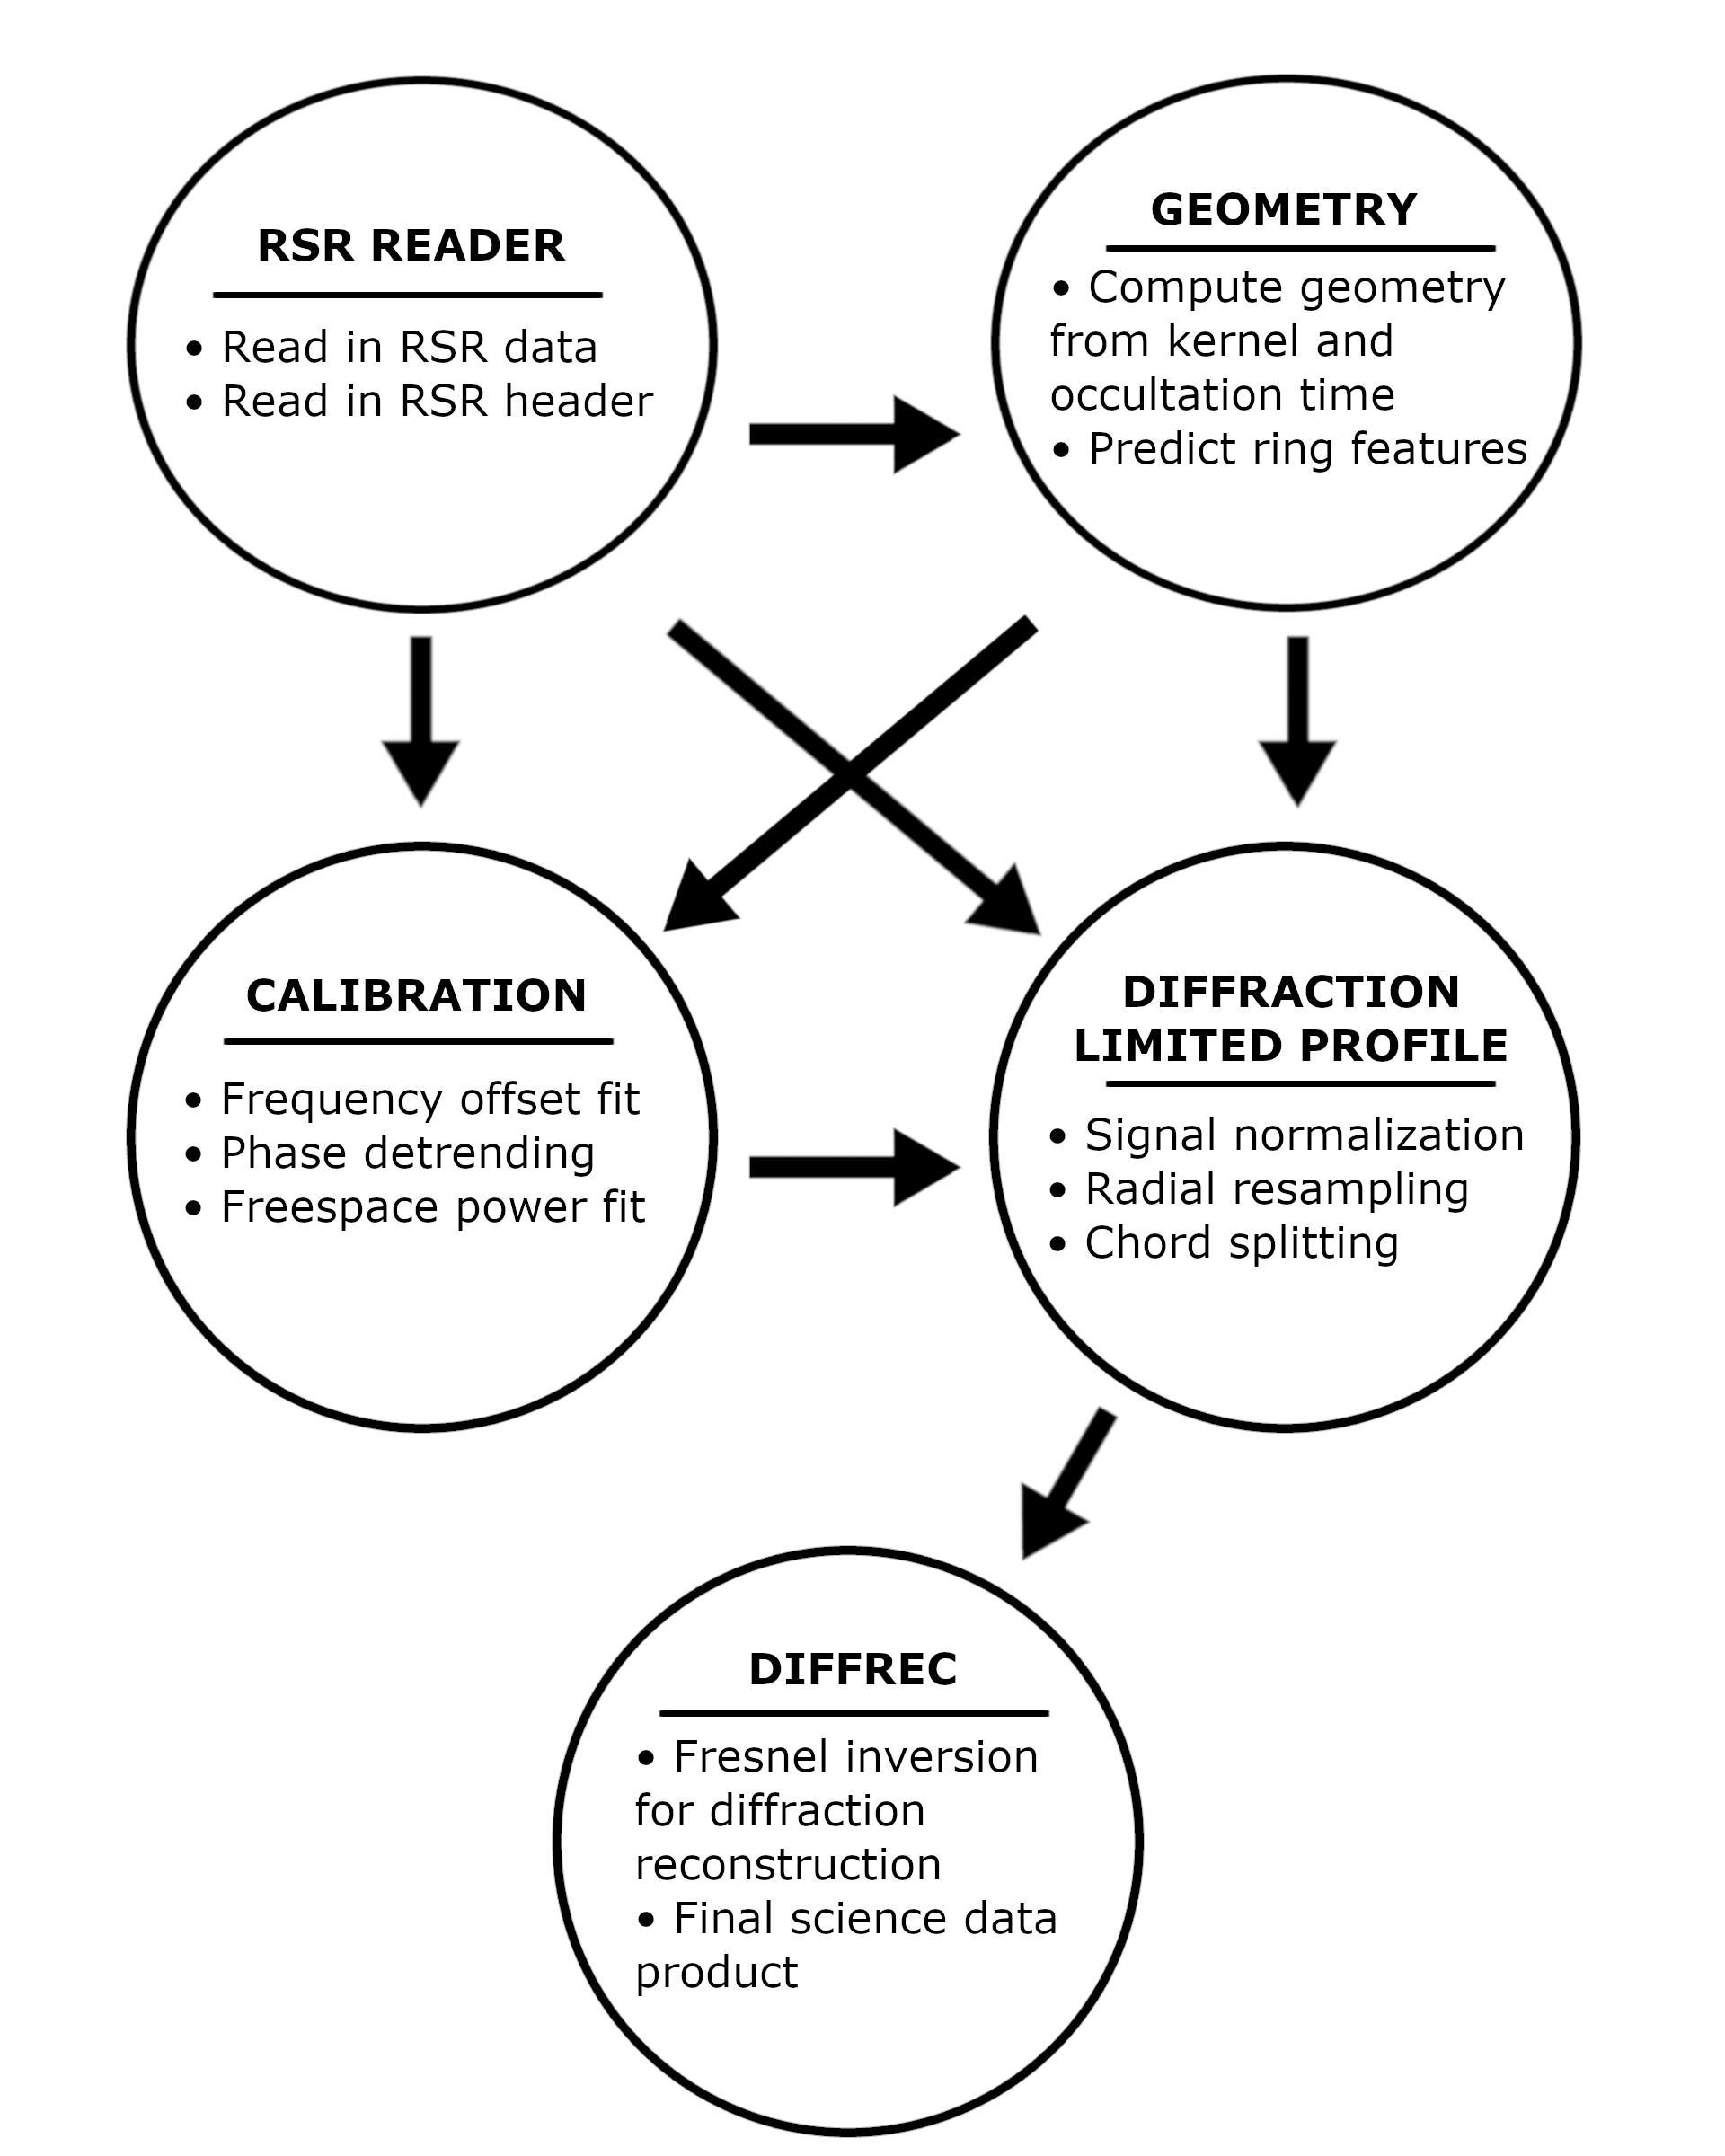
\includegraphics[width=\linewidth]{figs/ug_flowchart.png}
                \caption[Data processing pipeline]
                    {Data processing pipeline. Each bubble is a
                     separate object called by the \texttt{e2e*.py} scripts.}
                \label{fig:pipeline_schematic}
            \end{figure}
        \subsection{Conventions and hierarchy}
            Here, we list some conventions used in the
            \texttt{rss\_ringoccs} directory structure/hierarchy
            and the names of directories and output files.
            \begin{itemize}
                \item No reference is made within the
                      \texttt{rss\_ringoccs} package to local
                      directories outside of the top-level
                      \texttt{rss\_ringoccs/}
                      hierarchy of directories.
                \item The directory structure under
                      \texttt{rss\_ringoccs/}
                      \textit{must} strictly follow that of the
                      original download from the GitHub repository.
                \item For portability, all references within
                      \texttt{rss\_ringoccs}\ software to pathnames
                      to other directories within
                      \texttt{rss\_ringoccs/}
                      are relative, not absolute.
                \item Unless otherwise noted,
                      all executable scripts and Python programs
                      \textit{must} be run from within the
                      \texttt{rss\_ringoccs/pipeline/}
                      directory. (This is so that relative
                      pathnames will point to the correct
                      directories.)
                \item Output file names follow the format:\\
                      \texttt{RSS\_OBSY\_DOY\_B\#\#\_D\_%
                              INF\_RRRRRM\_YYYYMMDD\_XXXX.EXT}
                      \begin{itemize}
                          \item \texttt{OBSY} is the year the observation
                                was made
                          \item \texttt{DOY} is the day of the year
                                the observation was made
                          \item \texttt{B} is the wavelength band of the
                                observation
                          \item \texttt{\#\#} is the DSN station number
                          \item \texttt{D} is the direction of the
                                occultation
                          \item \texttt{INF} is a three-letter reference
                                specifying the information stored within
                                the file (\texttt{GEO} for the
                                occultation geometry,
                                \texttt{FOF} for the frequency offset,
                                \texttt{CAL} for calibration, \texttt{DLP}
                                for the DLP, and \texttt{TAU} for the
                                diffraction-reconstructed optical depth
                                profile)
                          \item \texttt{YYYYMMDD} is the year, month,
                                and date on which the user ran the
                                \texttt{rss\_ringoccs} code
                          \item \texttt{XXXX} is the \textit{XXXX}th
                                run of \texttt{rss\_ringoccs}
                                on that date
                          \item \texttt{EXT} is the file extension
                          \item Only DLP and TAU files contain the
                                \texttt{RRRRR} in the filename.
                                For the DLP
                                files, \texttt{RRRRR} is the minimum
                                reconstruction resolution (the so-called
                                ``DLP resolution" in MTR86)
                                in meters while
                                for TAU files this is the processing
                                resolution selected by the user
                          \item The output LBL files match those from
                                the PDS with minor changes.
                      \end{itemize}
            \end{itemize}
            With these caveats in mind, users are highly encouraged
            to write their own scripts to call upon and make full
            use of the \texttt{rss\_ringoccs} package. To that end,
            we provide example scripts for both pipeline versions
            as well as specific portions of the pipeline.
        \subsection{End-to-end pipeline: A look at the Huygens ringlet}
            \label{sec:end2end}
            The ``end-to-end'' pipeline process is a set
            of steps that need to be performed only once
            when processing a given RSR file from scratch.
            For the initial run, users will need
            to supply an RSR file, a set of kernels to use,
            a radial spacing to resample to, and a 
            reconstruction resolution (there are also default
            keyword inputs documented within each routine).
            The RSR extraction, geometry calculation, and frequency
            offset calculation steps are all automated; however,
            users may specify several options and parameters
            in advance by editing the input file \texttt{e2e\_run\_args.py}
            in the \texttt{./examples/} directory. These options
            include whether to process 16 kHz files, whether to write
            results to output files, whether to send output to the terminal,
            and whether the pipeline should enter
            an interactive mode to customize the freespace power
            fitting. This interactive mode will display the automated
            fit results in a \texttt{matplotlib} plotting window and
            prompt the user for changes to the fit parameters
            and/or freespace regions.
            \par\hfill\par
            At the end of the end-to-end run, if the \texttt{write\_file}
            keyword argument is set to \texttt{True}, several data files will
            be generated: geometry files, calibration files,
            diffraction-limited profile files, reconstructed optical
            depth files, and a summary file (in PDF format). Each class instantiated in
            the end-to-end pipeline process corresponds to a specific set
            of output files that match the format of those on the PDS produced by Essam Marouf. Once these files
            have been produced, users can use the quick-look process for
            subsequent runs.
            \par\hfill\par
            The pipeline's arguments file includes additional parameters for customizing the calibration steps
            and the profile ranges and resolutions. Detailed descriptions of which resolution values to choose and definitions of each
            type of resolution are given below.
            \par\hfill\par
            The following script illustrates the end-to-end pipeline by 
            producing a diffraction-corrected profile of Saturn's Huygens ringlet.
            To execute this script, follow the example below.
            \begin{lstlisting}[%
                language=bash,
                columns=fullflexible,
                basicstyle=\small\ttfamily,
                literate={~}{$\sim$}{1},
                frame=single,
                gobble=16
            ]
                cd rss_ringoccs/examples
                python e2e_run.py
            \end{lstlisting}
            This will automatically produce the multipanel plot shown in
            Fig.~\ref{fig:Huygens_ringlet}. The top row of plots show
            the raw power, optical depth, and phase profiles (i.e., the 
            observed diffraction pattern) that were
            input to \texttt{DiffractionCorrection}, and the bottom row
            shows the reconstructed radial profiles in power, optical depth and phase.
            \begin{figure}[ht]
                \centering
                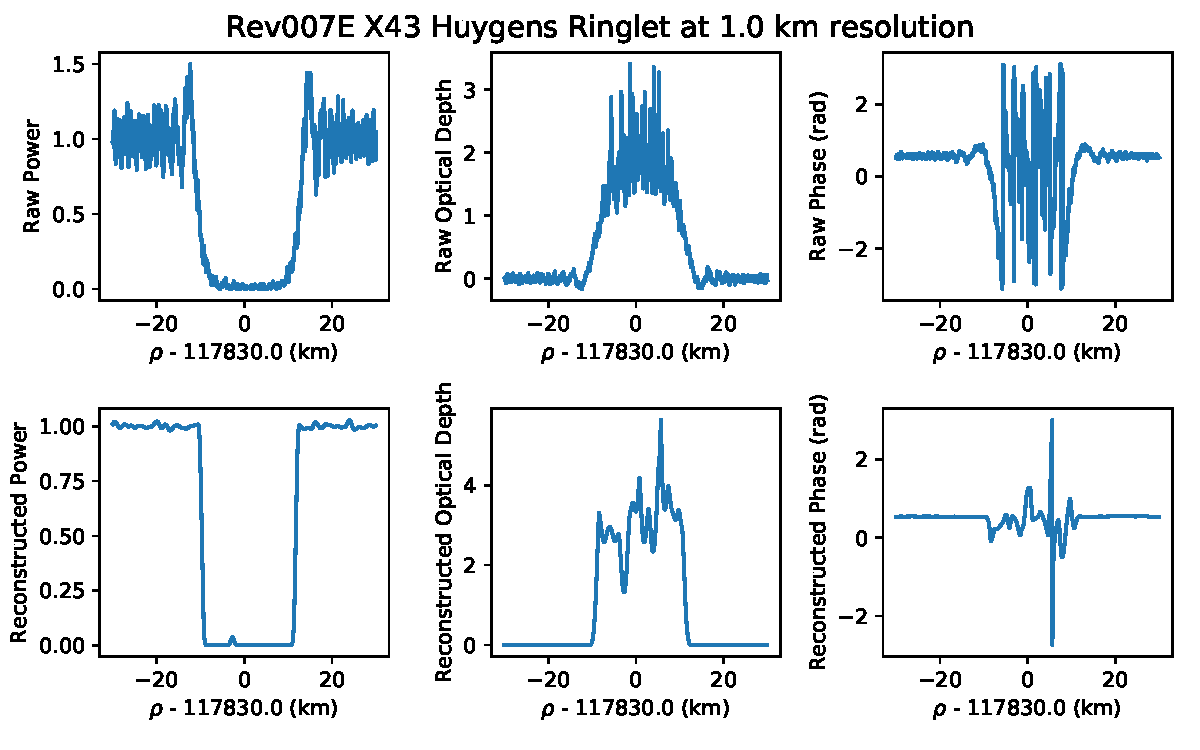
\includegraphics[%
                    trim = {0.in 0.0in 0in 0.0in},%
                    clip,%
                    width=\textwidth%
                ]{Rev007E_X43_Huygens_1km_20190123.pdf}
                \caption[Huygens ringlet initial testfigure]
                    {Power, optical depth, and phase plots
                     produced by e2e\_run.py} %Rev007EX43\_HuygensRinglet\_test.py}
                \label{fig:Huygens_ringlet}
            \end{figure}
        \subsection{Quick-look method: Comparing profiles
                    reconstructed at different resolutions}
            \label{sec:quicklook}
            The quick-look approach allows users to save computation
            time by utilizing pre-computed data files. For these runs, users
            start directly at the Fresnel inversion step of the pipeline,
            provided they have an appropriate set of \texttt{GEO*.TAB},
            \texttt{CAL*.TAB}, and \texttt{DLP*.TAB} files. Users must
            specify the relative file path(s) and desired \texttt{*.TAB}
            files to the \texttt{tools.ExtractCSVData()} class to create
            a DLP instance similar to the one instantiated in the end-to-end
            pipeline from the \texttt{calibration.DiffractionLimitedProfile()}
            class. This DLP instance can then be passed to the
            \texttt{diffrec.DiffractionCorrection()} class.
            \par\hfill\par
            Continuing with the RSR file downloaded in Section
            \ref{sec:getRSR}, we provide an example script to demonstrate
            diffraction-reconstructed optical depth profiles at different
            reconstruction resolutions for the Maxwell ringlet. Before
            running, users will need to open the \texttt{quick\_look\_run.py} script in a text editor
            and change line 15 from \texttt{date = 'YYYYMMDD'} to the date contained in the GEO, CAL, and DLP filenames. 
            For the first set of Rev007 files output by the
            \texttt{e2e\_run.py} script, this might resemble
            \begin{lstlisting}[
                language=python,
                columns=fullflexible,
                basicstyle=\small\ttfamily,
                literate={~}{$\sim$}{1},
                frame=single,
                gobble=16
            ]
                date = '20190629'
                data_dir = '../output/Rev007/Rev007E/Rev007E_RSS_2005_123_X43_E/'
                geo_file = data_dir+'RSS_2005_123_X43_E_GEO_' + date + '_0001.TAB'
                cal_file = data_dir+'RSS_2005_123_X43_E_CAL_' + date + '_0001.TAB'
                dlp_file = data_dir+'RSS_2005_123_X43_E_DLP_0100M_'+date + '_0001.TAB'
            \end{lstlisting}
            To execute the example quick-look script, follow the example below"
            \begin{lstlisting}[%
                language=bash,
                columns=fullflexible,
                basicstyle=\small\ttfamily,
                literate={~}{$\sim$}{1},
                frame=single,
                gobble=16
            ]
                cd rss_ringoccs/examples
                python quick_look_run.py
            \end{lstlisting}
            This will produce optical depth profiles at four different
            reconstruction resolutions: 1 km, 0.75 km, 0.5 km, and 0.25 km
            for the Rev007 egress X-band observation from DSS-43 processed by the
            end-to-end script in Section \ref{sec:end2end}. Running the
            script will produce a plot similar to Fig.~\ref{fig:maxwell_multi_res} (not including the reference red line for PDS data).
            \begin{figure}[!ht]
                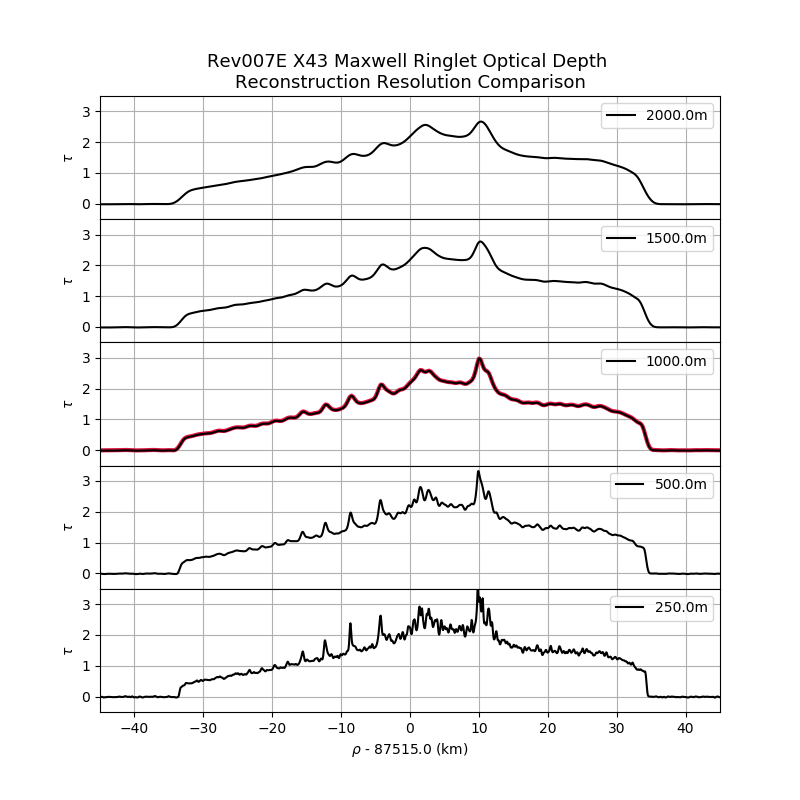
\includegraphics[width=\textwidth]
                    {figs/quicklook_tau.png}
                \caption[Rev007E Maxwell ringlet at different resolutions]
                    {%
                     Optical depth profile for the Maxwell ringlet from
                     the Rev007E X43 occultation reconstructed at 2 km,
                     1 km, 0.5 km, and 0.25 km resolution. Solid black lines
                     are the optical depth profile produced by the quick-look
                     example script at various processing resolutions indicated
                     by the plot text. For reference and validation, the solid
                     red line is the 1 km reconstruction resolution profile
                     obtained from the PDS3.%
                    }
                \label{fig:maxwell_multi_res}
            \end{figure}
        \subsection{Batch scripts}\label{sec:batchrun}
            To simplify and expedite the use of \texttt{rss\_ringoccs}
            to process large numbers of files, we provide a Python
            script \texttt{e2e\_batch.py} in the \texttt{pipeline} directory that
            runs the end-to-end pipeline for a list
            of files contained in a reference ASCII text file.
            The default list,
            \texttt{rsr\_1kHz\_files\_before\_USO\_failure.txt},
            is the same list of files used by \texttt{get\_rsr\_files.sh}
            to download all of the 1 kHz Cassini RSR files prior to
            the USO failure, and can be found in the
            \texttt{tables/} directory. This batch script, like the single-
            file script, reads in a file of parameters, 
            \texttt{e2e\_batch\_args.py}, which specifies, among
            other things, radial sampling rates, calibration fit orders, 
            profile range, and whether to output files.
            By modifying the contents of
            \texttt{e2e\_batch\_args.py}, users can produce
            on-demand, customized optical depth profiles for specific data sets and radial regions of interest.
            Each option within \texttt{e2e\_batch\_args.py} is documented
            in comments. For more information, we refer users to either \S\ref{sec:detailedlook} or the documentation online at 
            \url{https:\\rss-ringoccs.readthedocs.io}.
            \par\hfill\par
            The default end-to-end pipeline will jump into its interactive
            mode when the automated normalization of the received power to a nominal free-space level 
            is poor. To avoid this
            interactive mode, one can alternatively run the script prepended with
            the unix \texttt{yes} command to automatically enter the string
            ``yes" for all input prompts (thus accepting the default fit,
            should \texttt{rss\_ringoccs} enter interactive mode). Running
            the batch script in this manner will resemble
            \begin{lstlisting}[%
                language=bash,
                columns=fullflexible,
                basicstyle=\small\ttfamily,
                literate={~}{$\sim$}{1},
                frame=single,
                gobble=16
            ]
                yes | python e2e_batch.py
            \end{lstlisting}
           The end-to-end Python script will automatically generate an error log file with a name such as 
            \texttt{e2e\_batch\_YYYYMMDD-HHMMSS.err}  
            to contain names of files that failed
            to process during the batch run as well as the resulting traceback
            error. If \texttt{verbose} keyword argument is set to
            \texttt{True}, some benign messages, such as:\\
            \\
            \begin{lstlisting}[%
                language=bash,
                columns=fullflexible,
                basicstyle=\small\ttfamily,
                literate={~}{$\sim$}{1},
                frame=single,
                gobble=16
            ]
                1) WARNING (RSRReader): file size not the same as expected!
                2) DETECTED INGRESS (resample_IQ.py): reversing arrays
            \end{lstlisting}
            will be printed to the terminal. These do not result in failed processing runs and are therefore not printed to the \texttt{.err} file.
            \par\hfill\par
            One of the default parameters is
            \texttt{with16=False}, which skips 16 kHz files that have no
            corresponding 1 kHz files (see \S\ref{sec:getRSR}, Table
            \ref{tab:missing files from PDS}). Set this to \texttt{True} only if
            the user's computer has at least 16 GB RAM; these files will also take
            longer to process than a typical 1 kHz file.
            
            \par\hfill\par
            \texttt{rss\_ringoccs} provides several additional end-to-end scripts to illustrate batch processing:
            \begin{itemize}
                \item From the \texttt{pipeline} directory, run this batch file for a 1 km reconstruction of occultations prior to USO failure. (This is identical to the default version of \texttt{e2e\_batch.py}, except that all of the parameters for the batch run are included at the top of the source file, instead of being contained in a separate file such as \texttt{e2e\_batch\_args.py}.) Execution time may vary with local hardware. Anticipate at least 3.5-4 hrs for this script to run.
    \begin{lstlisting}[%
        language=bash,
        columns=fullflexible,
        basicstyle=\footnotesize\ttfamily,
        frame=single,
        escapechar=",
        gobble=8]
        yes | python e2e_batch_1km.py
    \end{lstlisting}
    \item From the \texttt{pipeline} directory, run this batch file for a 500 m reconstruction of occultations prior to USO failure.  Execution time may vary with local hardware. Anticipate at least 15 hrs for this script to run.
    \begin{lstlisting}[%
        language=bash,
        columns=fullflexible,
        basicstyle=\footnotesize\ttfamily,
        frame=single,
        escapechar=",
        gobble=8]
        yes | python e2e_batch_500m.py
    \end{lstlisting}
    \item For a 1 km reconstruction of occultations post-USO failure, run this batch file. Execution time may vary with local hardware. Anticipate at least 10 hrs for this script to run.
    \begin{lstlisting}[%
        language=bash,
        columns=fullflexible,
        basicstyle=\footnotesize\ttfamily,
        frame=single,
        escapechar=",
        gobble=8]
        yes | python e2e_batch_postUSO_1km.py
    \end{lstlisting}
\end{itemize}
We strongly recommend that users not run simultaneous end-to-end batch jobs that use the same set of input RSR files, since this could result in inconsistent version numbers for the output files or overwriting/deletion of intermediate files that are normally hidden from the user.

        \subsection{Profile resolution}\label{sec:resolutions}
        As a practical matter, most users would like to know: ``What is the highest achievable resolution for a given ring occultation, and how can I use \texttt{rss\_ringoccs} to produce a radial profile at that resolution?"
        The answer is complicated by a variety of definitions of resolution -- we clarify these below -- and is also affected of course by the SNR of any given occultation, which depends on the wavelength of the observation, the observing conditions at the DSN, the size of the receiving antenna, the geometry and speed of the occultation, and host of other factors. 
        \par\hfill\par
        We recommend that users begin with the 1-km reconstructions already available on the PDS, to get a sense for the signal quality of a specific occultation of interest. As a next step, we provide an end-to-end script that uses \texttt{rss\_ringoccs} to process the entire set of Cassini RSS occultation data (up to the point of the USO failure) at a diffraction-corrected resolution of 0.5 km. Users can compare these profiles with the 1.0 km results available on the PDS, and decide whether reconstruction at a different resolution is needed. 
              \par\hfill\par
        In cases where higher resolution is desired and is warranted by the SNR, we recommend that \texttt{rss\_ringoccs} users produce diffraction-reconstructed radial profiles at successively finer resolutions (centered on a feature of interest over a limited radial range to reduce processing time). As the resolution is increased, the effects of noise will eventually limit the useful information that can be obtained for a particular science goal.
        \par\hfill\par
        To carry this out in practice, it is important to understand the factors that affect the diffraction-reconstructed resolution.
        Prior to diffraction reconstruction, RSS observations are limited in resolution  at a spatial scale comparable to the Fresnel scale $F\approx\sqrt{\lambda D/2}$, where $\lambda$ is the wavelength of observation and $D$ is the distance between the spacecraft and the ring plane. Geometrical effects such as the tilt of the ring plane result in multiplicative scale factors applied to $F$, when converted to an effective diffraction-limited resolution in the radial direction in the ring plane. As a general rule, the effective Fresnel scale for RSS ring measurements is of order a few km for typical occultations. 
        \par\hfill\par
        The task of diffraction reconstruction is to improve on the diffraction-limited resolution of the observations by making use of both the intensity and phase of the received signal across the diffraction pattern. Intuitively, it makes sense that a high-resolution diffraction reconstruction will require finer resolution of the observed diffraction pattern, over a larger radial range (what we refer to as a \textit{filter window} -- see MTR86 for details), than a low-resolution reconstruction. For sub-km diffraction reconstruction at S-band (the longest of the three Cassini wavelengths), the filter window can extend for hundreds of km to either side of the location of the feature of interest, and it must be sampled at a fine enough spatial scale to capture the structure of fine-scale diffraction fringes produced by the ring feature over the entire filter window.
          \par\hfill\par
        From these considerations, it is clear that in order to achieve a given post-reconstruction resolution, there is an implied requirement on the resolution at which the diffraction-limited profile is calculated. To satisfy the sampling theorem, if the radial sampling of the diffraction-limited DLP profile is $\Delta\rho$, the subsequent diffraction reconstruction resolution can only 
        have shortest resolvable wavelengths of Nyquist or higher (i.e., 
        $\ge2\Delta\rho$) -- more on this in a moment! As a practical matter, it sometimes makes sense to produce a DLP profile once and for all at very high resolution (say, 0.05 km), use it to produce a diffraction-reconstructed profile at, say, 1 km resolution, and then to reuse this same DLP profile to explore the SNR properties of successively higher resolution diffraction reconstructions, consistent with the sampling theorem.
        \par\hfill\par
        The original data are recorded at regular intervals in time, but most of our processing is done as a function of ring plane radius.
        To achieve uniform radial sampling, we take account of the changing velocity and trajectory of the spacecraft and resample the phase-corrected complex
        signal at a user-defined spacing $\Delta\rho$ (passed to the 
        \texttt{DiffractionLimitedProfile} as the positional argument \texttt{dr\_km}
        when instantiating the class). We 
        suggest a value for \texttt{dr\_km} no smaller than 0.05 km.
        \par\hfill\par
        To satisfy the sampling 
        theorem, the subsequent diffraction reconstruction resolution can only 
        have shortest resolvable wavelengths of Nyquist or higher (i.e., 
        $\ge2\Delta\rho$). However, the situation is complicated by a variety of definitions of diffraction reconstruction resolution. As MTR86 point out (see Eqs.~10--14), resolution can be defined in terms of the the filter window width $W$ either as the null-to-null width of the main diffraction lobe, or as the equivalent width of the normalized impulse response profile -- these definitions differ by a factor of two from each other. Uncertainty in the Fresnel scale can further degrade the effective resolution, as can limitations on the validity of the approximations made to compute the phase of the signal. 
         \par\hfill\par
        In our development of \texttt{rss\_ringoccs}, we used the MTR86 Eq.~11 definition of effective resolution $\Delta R_W=2F^2/W$ and the geometrically scaled definition of $F$ given by MTR86 Eq.~6. This is the definition used throughout MTR86 in the analysis of Voyager RSS data, and it matches our results when we apply diffraction reconstruction to the archived PDS Voyager Saturn and Uranus RSS diffraction-limited profiles. We refer to this as the \textit{processing resolution} $\Delta R$ within \texttt{rss\_ringoccs}.
        \par\hfill\par
        In contrast to these conventions, Essam Marouf introduced a different definition of resolution in his Cassini reconstructed profiles available on the PDS, based on applying a low-pass filter to the diffraction reconstruction. The relation between $\Delta R_W$  and this new PDS definition of resolution is given by
        $$\Delta R_W = 0.75 \Delta R_{\rm PDS}$$
        or
        $$\Delta R_{\rm PDS} = \frac{4}{3} \Delta R_W.$$
           \par\hfill\par
        Given these two definitions, and a lack of information about the details of the low-pass filter used by Marouf, we faced a choice: should we retain the definition of resolution as derived in MTR86 and apparently used for Voyager RSS results, or should we be consistent with the recent PDS contributions by Marouf? We chose the latter approach, so that our \texttt{rss\_ringoccs} runs of Cassini RSS observations were consistent with, and could be directly compared to, the PDS results at the same quoted post-reconstruction resolution. The user specifies a desired resolution $\Delta R_{\rm PDS}$ for the reconstructed profile
        through the \texttt{res} positional 
        argument when instantiating the \texttt{DiffractionCorrection} class. The 
        resolution specified by \texttt{res} is then scaled within this class
        to the processing 
        resolution $\Delta R$ by the factor of 0.75 described above. 
        \par\hfill\par
        In our interpretation of the sampling theorem, \texttt{rss\_ringoccs} requires that $\Delta R_W > 2\Delta\rho$. In terms of the requested diffraction-corrected resolution $\Delta R_{\rm PDS}$, this places the following restriction on the pre- and post-diffraction reconstructed resolutions:
        $$\Delta R_{\rm PDS}> \frac{8}{3}\Delta\rho.$$
        \par\hfill\par
        The factor of 8/3 is non-intuitive, but is the best compromise we could find. As  specific example, for a DLP file produced at 0.05 km resolution ($\Delta\rho=0.05$ km), the requested post-diffraction resolution $\Delta R_{\rm PDS}$ (or \texttt{res}) must be no smaller than $8/3\times0.05 = 0.133$ km. (This is below the useful resolution of the majority of Cassini RSS ring observations.) If the user violates these conditions, an informative error message will be displayed, made more comprehensible (we hope!) by this  discussion.
    \section{A detailed look at \texttt{rss\_ringoccs}}\label{sec:detailedlook}
        Here, we elaborate on the inner workings of \texttt{rss\_ringoccs},
        describing the methods and goals of each step of the software pipeline.
        For documentation and definition of individual variables, functions,
        methods, and modules, we refer the user to our online reference available
        at \url{https://rss-ringoccs.readthedocs.io/en/master/}.
        \subsection{RSR reader}
            The \texttt{rsr\_reader/} subpackage is used
            for extracting information from a given RSR file.
            The \texttt{RSRReader} class, when instantiated with
            a linked RSR file, extracts the raw complex signal $I$
            and $Q$  from the RSR file from the PDS as well as some
            accompanying non-geometric meta-data stored in the RSR
            file header such as the DSN station, observation dates,
            sampling rate, start and end times of the observation,
            and the band of observation.
        \subsection{Occultation geometry routines}
            The routines in \texttt{occgeo/} depend heavily on the
            NAIF SPICE Toolkit and are geared towards reproducing
            all occultation geometry parameters that are documented within
            \texttt{Archived\_Cassini\_RSS\_RingOccs\_2018},
            or \texttt{CORSS\_8001 v2}, submission
            (see Table~\ref{tab:easydata_glossary_of_geo_file}).
            In addition to these parameters, \texttt{Geometry}
            also calculates %the elevation angle of the observation
            %at the DSN station, 
            the optical depth enhancement
            factor $\beta$ and the effective ring opening angle $B_{eff}$. (See the documentation in the source code \texttt{rss\_ringoccs/occgeo/calc\_occ\_geometry.py} for the definitions of these quantities.)
            \par\hfill\par
            Using orbital parameters compiled from literature and the computed
            ring azimuth and ring radius, \texttt{Geometry} uses the
            \texttt{find\_gaps} method from the \texttt{cal\_occ\_geo} module
            to determine the locations of gaps in the ring system in the
            occultation data set. This is done iteratively by repeating the
            following steps, choosing the semimajor axis of the gap edge for
            the initial predicted edge radius:
            \begin{enumerate}
                \item Find the ring radius in the occultation data set
                      closest to the predicted gap edge radius.
                \item Find the ring azimuth and orbital time implied by
                      the closest ring radius.
                \item Predict the radius of the gap edges using compiled
                      orbital properties and the implied ring azimuth and time.
            \end{enumerate}
            \begin{table}[H]
                \centering
                \begin{tabular}{l l l} 
                    \hline
                    Symbol&Parameter Name
                          &\texttt{Geometry} Attribute\\
                    \hline
                    $t_{OET}$&OBSERVED EVENT TIME
                             &t\_oet\_spm\_vals\\
                    $t_{RET}$&RING EVENT TIME
                             &t\_ret\_spm\_vals\\
                    $t_{SET}$&SPACECRAFT EVENT TIME
                             &t\_set\_spm\_vals\\
                    $\rho$&RING RADIUS
                          &rho\_km\_vals\\
                    $\phi_{RL}$&RING LONGITUDE
                               &phi\_rl\_deg\_vals\\
                    $\phi_{ORA}$&OBSERVED RING AZIMUTH
                                & phi\_ora\_deg\_vals\\
                    $B$&OBSERVED RING ELEVATION
                       &B\_deg\_vals\\
                    $D$&SPACECRAFT TO RING INTERCEPT DISTANCE
                       &D\_km\_vals\\
                    $V_{rad}$&RING INTERCEPT RADIAL VELOCITY
                             &rho\_dot\_kms\_vals\\
                    $V_{az}$&RING INTERCEPT AZIMUTHAL VELOCITY
                            &phi\_rl\_dot\_kms\_vals\\
                    $F$&FRESNEL SCALE
                       &F\_km\_vals\\
                    $R_{imp}$&IMPACT RADIUS
                             &R\_imp\_km\_vals\\
                    $r_x$&SPACECRAFT POSITION X
                         &rx\_km\_vals\\
                    $r_y$&SPACECRAFT POSITION Y
                         &ry\_km\_vals\\
                    $r_z$&SPACECRAFT POSITIION Z
                         &rz\_km\_vals\\
                    $v_x$&SPACECRAFT VELOCITY X
                         &vx\_kms\_vals\\
                    $v_y$&SPACECRAFT VELOCITY Y
                         &vy\_kms\_vals\\
                    $v_z$&SPACECRAFT VELOCITY Z
                         &vz\_kms\_vals\\
                    $\theta_{EL}$&OBSERVED SPACECRAFT ELEVATION
                                 &elev\_deg\_vals \\ 
                    \hline
                \end{tabular}
                \caption[Glossary of parameters in the *GEO.TAB file]
                    {Glossary of parameters in *GEO.TAB file
                     in PDS submission
                     \texttt{Cassini\_RSS\_Ring\_Profiles\_2018\_Archive}
                     and their corresponding attribute names
                     within the \texttt{Geometry} class.}
                \label{tab:easydata_glossary_of_geo_file}
            \end{table}
            This iterative process returns the gap edge radius once it converges
            to a solution (i.e., when the difference between two consecutive
            radius predictions is less than one meter) which occurs within five
            iterations or less. The inner and outer edges of each gap are then
            stored as an attribute of the \texttt{Geometry}
            object instance for future use.
            \par\hfill\par
            To create an instance of \texttt{Geometry}, or
            \texttt{geo\_inst}, users will need an instance of
            the \texttt{RSRReader} class (\texttt{rsr\_inst}),
            a target planet, a target spacecraft, a set of kernels
            over the duration of the RSR file used in
            \texttt{rsr\_inst}, and, optionally, a desired number
            of points per seconds for all calculations
            (the default is 1 point per second). For choosing an
            RSR file, which is the only input necessary for
            instantiating \texttt{RSRReader}, see Section
            \ref{choose_rsr}.
    \subsection{Calibration routines}\label{sec:calroutines}
            All of the routines needed to produce a calibrated diffraction
            pattern are in the \texttt{calibration/} directory in the
            \texttt{rss\_ringoccs} package. Each of them performs a
            portion of the frequency and power calibration steps. Every step
            of the calibration process is handled by the \texttt{Calibration}
            class. When instantiated (which requires the appropriate instances
            of the \texttt{RSRReader} and \texttt{Geometry} classes), it calls
            the \texttt{FreqOffsetFit} class to compute the offset frequency
            needed for phase-correcting the measured complex signal. Then, the
            signal is phase-corrected using the \texttt{Calibration} class
            method \texttt{correct\_IQ} following \citet{Marouf1986} and
            \citet{CRSUG2018}. The phase detrending function $\psi$ is
            computed from the cumulative integral:
            \begin{equation}
                \psi=\int^{t}\hat{f}(\tau)_{offset}\diff{\tau}+\psi(t_0)
            \end{equation}
            and used for detrending the complex signal such that:
            \begin{equation}
                I_{c}+iQ_{c}=[I_{m}+iQ_{m}]\exp(-i\psi)
            \end{equation}
            \citep[Equations 17 and 18]{CRSUG2018}.
            Then, \texttt{Calibration} normalizes the phase-corrected signal,
            using the \texttt{Normalization} class to estimate the intrinsic
            spacecraft power $\hat{P}_0$ as it changes over the course of the
            occultation.%
            \footnote{Limits on the reliability of the normalized
                      power are estimated in the form of threshold
                      optical depth,
                      \par\hspace{1.3ex}
                      which is computed by the
                      \texttt{calc\_tau\_thres} class when instantiating
                      \texttt{DiffractionLimitedProfile()}.}
            Finally, all the results of the calibration are written out to
            an \texttt{LBL} and a \texttt{TAB} file following the naming
            conventions discussed above.
            \subsubsection{Frequency offset}
            \label{subsubsec: freq_offset}
                To estimate the offset frequency over the entire
                occultation, we compute the offset frequency $f(t)_{offset}$
                directly from the raw data using a series of ``rolling-window"
                FFTs. This is stored
                as an attribute of the \texttt{FreqOffsetFit} class for use by
                the phase detrending method in the \texttt{Calibration} class.
                Beginning with V1.2 of \texttt{rss\_ringoccs}, \texttt{FreqOffsetFit} deviates from previous approaches to
                fitting the frequency offset residual for several reasons: 
                \begin{enumerate}
                \item Some RSR files contain NANs in the file headers in place of the
                coefficients needed for calculating the polynomials that describe
                the predicted sky frequency, which prevented computing the residual
                frequency offset. 
                \item Computing the predicted sky frequency over
                the entire occultation added at least 5 seconds of computation time
                to each of the 151 RSR files at 1 kHz prior to USO failure. 
                \item Primarily for post-USO failure observations, disagreements between the predicted and reconstructed sky frequency
                sometimes exceeded 2 MHz and introduced scalloping into the frequency
                offset, which prevented appropriate description of the frequency offset.
                \item Systemically, there is essentially no difference between fitting
                the frequency offset and the residual frequency offset. 
                \end{enumerate}
                Our new approach not only simplifies the pipeline
                but also enables support for processing many more files than
                previously possible.
                \par\hfill\par
                When instantiated, the \texttt{FreqOffsetFit} class begins by
                instancing the \texttt{calc\_freq\_offset} class, which
                contains methods to calculate the frequency offset as a
                function of time from the raw data. It uses the time
                (\texttt{spm\_vals}) and raw signal $I_m+iQ_m$ (\texttt{IQ\_m})
                attributes of RSRReader class (\texttt{rsr\_inst}). Its
                positional arguments are an instance of the RSRReader class
                (\texttt{rsr\_inst}) and two floats specifying the minimum and
                maximum \gls{spm} values to use as limits on the range of occultation
                data for which the offset frequency is computed (this reduces
                computation time by eliminating the calculation of offset
                frequencies that are not useful for constraining the signal offset
                frequency). Its optional inputs are \texttt{dt\_freq}
                for the FFT window size in seconds from which to calculate
                frequency offset (default is 2 seconds) and
                \texttt{verbose} for a Boolean specifying whether to print out
                intermediate steps to the terminal (default is \texttt{False}).
                \par\hfill\par
                To calculate the frequency offset from the data, we use the
                \texttt{numpy} FFT module to compute the frequency components of
                the raw measured complex signal for a window in time with a width
                of \texttt{dt\_freq} and centered on time \texttt{spm\_mid}. The submodule \texttt{calc\_freq\_offset}
                estimates the frequency corresponding to the peak in the power
                spectrum near the center of the bandpass in two
                steps. First, it takes a discrete approach by applying a Hamming
                filter to the signal within the window, computing the
                discrete FFT, and obtaining the frequency associated
                with the maximum power ($|A^2|/N$). Second, to better
                constrain the frequency offset,
                \texttt{calc\_freq\_offset} takes a continuous
                approach, computing the
                continuous Fourier transform of the Hamming-filtered complex signal
                at a 0.001 Hz sampling in frequency over
                a 0.5 Hz window centered on the peak frequency
                found in the discrete Fourier transform. The
                frequency associated with the maximum power
                ($|A^2|/N$) of the continuous Fourier transform is taken to be the carrier frequency offset associated with the time \texttt{spm\_mid}. The
                result is stored in an array. Then, the window center is shifted
                forward in SPM by the sampling resolution value, and the process
                is repeated. The first window is centered at the initial SPM value
                plus half with window width and is sampled at the
                keyword-specified resolution until the window center is half a
                window width from the end of the time series.
                \par\hfill\par
                \begin{table}[H]
                    \centering
                    \begin{tabular}{l l l}
                        \hline
                        Symbol&Parameter Name
                              &\texttt{Calibration} Attribute\\
                        \hline
                        $t_{OET}$&OBSERVED EVENT TIME
                                 &t\_oet\_spm\_vals\\
                        $\hat{f}(t)_{sky}$&SKY FREQUENCY
                                 &f\_sky\_hz\_vals\\
                        $\hat{f}(t)_{offset}$&OFFSET FREQUENCY
                                   &f\_offset\_fit\_vals\\
                        $\hat{P}_{0}$&FREESPACE POWER
                                  &p\_free\_vals \\
                        \hline
                    \end{tabular}
                    \caption[Glossary of data from the CAL file]
                        {Glossary of calibration data in the CAL files.}
                    \label{tab:easydata_glossary_from_cal_file}
                \end{table}
                \par\hfill\par
                The \texttt{FreqOffsetFit} class then calls
                \texttt{calc\_f\_sky\_recon}, a pythonized version of Nicole Rappaport's \textsc{Predicts} Fortran software, to compute the reconstructed sky
                frequency. This uses spacecraft ephemerides available in the
                kernel files and \texttt{spiceypy} to determine the implied line-of-sight Doppler
                shift of the intrinsic USO frequency due to the motion of the 
                spacecraft relative to the observing station. This gives a
                reconstructed sky frequency, denoted as $f(t)_{dr}$.
                \par\hfill\par
                With its method \texttt{create\_mask}, \texttt{FreqOffsetFit}
                performs sigma clipping of the offset frequency to
                exclude unreliable data by creating a boolean mask
                array. The method begins by masking out all offset frequencies
                more than five standard deviations away from the median
                frequency offset. Then, this method fits the masked data using
                the \texttt{calc\_polyorder}. This method fits data with polynomials of
                iteratively increasing order, using the F-test statistic to evaluate
                whether a higher order polynomial provides a statistically significantly better fit to the frequency
                offset data. The method stops when increasing the polynomial order
                does not provide a better description or when the polynomial order
                exceeds nine. The \texttt{create\_mask} method uses this ``best fit"
                polynomial to perform a second-order sigma clipping by excluding data 
                which are more than five standard deviations away from the ``best fit" 
                polynomial.
                \par\hfill\par
                In order to exclude spurious inclusion, \texttt{create\_mask}
                performs a ``nearest-neighbor" comparisons. The first comparison
                examines the four nearest data points included by the boolean mask. If
                the absolute difference between the considered datum and each of its
                four neighbors exceeds 0.25 Hz, the datum is excluded. The second 
                comparison assumes any datum with at least four excluded nearby data
                points should also be excluded. Finally, a boolean mask array is returned 
                that excludes all unreliable data.
                \par\hfill\par
                \texttt{FreqOffsetFit} uses its \texttt{fit\_f\_sky\_offset}
                method to fit a polynomial (of order specified by the \texttt{calc\_polyorder}
                method to prevent over-fitting) to the masked frequency
                offset data using the \texttt{numpy.polynomial} subpackage. The
                best-fit polynomial $\hat{f}(t)_{offset}$ is returned along with
                the reduced summed squared residuals as an estimate of the fit
                quality.
                \par\hfill\par
                \texttt{FreqOffsetFit}
                computes $\hat{f}(t)_{offset}$ and stores both the
                $\hat{f}(t)_{dr}$ and $\hat{f}(t)_{offset}$
                variables as attributes.
                For reference and visual assessment, \texttt{FreqOffsetFit}
                plots the total and sigma-clipped sets of $f(t)_{offset}$ and
                overplots $\hat{f}(t)_{offset}$. The plot is saved in the
                appropriate output directory and is named following the
                \texttt{*.TAB} and \texttt{*.LBL} conventions with the infix
                \texttt{FORFIT}.
            \subsubsection{Power normalization}
                After phase compensation of the complex signal, the
                \texttt{Calibration} class instantiates the
                \texttt{Normalization} class. The objective of this class is
                to estimate the intrinsic spacecraft signal power $\hat{P}_0$
                by fitting the observed power in free space regions with a
                low-order polynomial. A \texttt{Normalization} instance requires
                $I_c+iQ_c$ and an instance of the \texttt{Geometry} class
                (\texttt{geo\_inst} in the pipeline scripts).
                \par\hfill\par
                To begin, \texttt{Normalization} down-samples the corrected
                complex signal by a factor of 500. This serves to minimize the
                effect of extended ring diffraction patterns in the free space regions
                on the overall prediction of $\hat{P}_0$ while expediting the
                fitting procedure.
                \par\hfill\par
                Next, \texttt{Normalization} utilizes the ring gaps and other
                free space regions predicted by the \texttt{find\_gaps} function
                in the \texttt{calc\_occ\_geo} submodule in units of SPM. Free
                space regions are then excluded or retained by comparing the
                median power within the SPM limits of the free space region to
                the maximum power \textit{within} the ring system. Because
                extinction by the ring material causes a decrease in observed
                signal power, this effectively selects the maximum power observed
                in gaps and divisions inside of the ring system. When the median
                power within a given free space region is 50\% below or 25\%
                above the maximum ring-system spacecraft signal power, the data
                from this free space region are excluded. After these comparisons
                and rejections are made, data from all remaining free space
                regions are assembled for use in a polynomial fit.
                \par\hfill\par
                The \texttt{Normalization} method 
                \texttt{fit\_freespace\_power} then fits these reliable measurements
                of the intrinsic spacecraft signal in order to estimate
                $\hat{P}_0$ over the entire occultation. The default fit is a
                third order polynomial; however, the fit order can be changed
                when instantiating the \texttt{Calibration} class using the
                keyword argument \texttt{pnf\_order} and the fit type can be
                set using the keyword argument \texttt{pnf\_fittype}
                (default of ``poly" for polynomial and ``spline" for spline,
                piece-wise is on lien for future versions). Regardless of user
                input, if the number of free space regions is less than five,
                the fitting method forces the fit order to linear.
                \par\hfill\par
                If the keyword \texttt{interact} is set to \texttt{True} 
                when instantiating the \texttt{Calibration} instance,
                \texttt{Normalization} will enter its interactive mode after
                computing the best fit to the reliable free space data. In this
                mode, users can customize the free space regions, fit type, and
                fit order following prompts in the terminal.
                The command line will prompt the user to confirm interactive
                mode and subsequently display a plot in a
                \texttt{matplotlib.pyplot} window showing the best-fit
                polynomial to the default free space regions. Both the individual
                regions and the total profile will be displayed so that the
                user may assess the quality of the fit (in the same manner as
                the output fit plot, as shown in Figure \ref{fig:fspfit_examp}).
                The command line will then prompt users whether to change
                included free space regions or revert to the defaults generated
                by the automated pipeline (see Appendix \ref{app:interact}
                for an example). If the user opts to change the free space
                regions, new definitions for the desired free space regions
                (specified as pairs of lower and upper SPM limits for each region)
                will need to be entered in the following format
                \begin{equation*}
                    \texttt{[[30500,31785],[34080,34245],[35285,36000]]}
                \end{equation*}
                to be used in the fit. If the new free space region limits
                are not entered in the appropriate format, the code will
                revert to the initial freespace regions predicted
                by \texttt{Geometry}.
                \par\hfill\par
                Once the final fit has been computed, $\hat{P}_0$ and the
                boundaries of the free space regions used to compute the fit
                are stored as attributes. As with the frequency offset
                fit, this step also includes plotting the fit results for
                visual inspection and reference. $\hat{P}_0$ is plotted over
                the phase-compensated signal power for both the entire profile
                and for each individual free space region used in the fit.
                Naming convention follows that of the \texttt{*.TAB} and
                \texttt{*.LBL} files with the infix \texttt{FSPFIT}.

        \subsection{Diffraction-limited profile routines}
            \begin{table}[H]
                \centering
                \resizebox{\textwidth}{!}{%
                    \begin{tabular}{l l l}
                        \hline
                        Symbol&Parameter Name&
                        \texttt{NormDiff} Attribute\\
                        \hline
                        $\rho$&RING RADIUS&rho\_km\_vals\\
                        $\Delta\rho_{IP}$&RADIUS CORRECTION DUE TO IMPROVED POLE
                                         &rho\_corr\_pole\_km\_vals\\
                        $\Delta\rho_{TO}$&RADIUS CORRECTION DUE TO TIMING OFFSET
                                         &rho\_corr\_timing\_km\_vals\\
                        $\phi_{RL}$&RING LONGITUDE&phi\_rl\_rad\_vals\\
                        $\phi_{ORA}$&OBSERVED RING AZIMUTH&phi\_ora\_rad\_vals\\
                        $\tau$&NORMAL OPTICAL DEPTH&tau\_norm\_vals\\
                        $\phi$&PHASE SHIFT&phase\_rad\_vals\\
                        $\tau_{TH}$&NORMAL OPTICAL DEPTH THRESHOLD
                                   &tau\_threshold\_vals\\
                        $t_{OET}$&OBSERVED EVENT TIME&t\_oet\_spm\_vals\\
                        $t_{RET}$&RING EVENT TIME&t\_ret\_spm\_vals\\
                        $t_{SET}$&SPACECRAFT EVENT TIME&t\_set\_spm\_vals\\
                        $B$&OBSERVED RING ELEVATION&B\_rad\_vals\\
                        \hline
                    \end{tabular}
                }
                \caption[Glossary of parameters in TAU file]{%
                    Glossary of optical depth, phase shift,
                    and selected geometry parameters
                    contained in the DLP files.
                }
                \label{tab:easydata_parameters_from_dlp_file}
            \end{table}
            When instantiated, the \texttt{DiffractionLimitedProfile} class
            normalizes the power profile using the results from the
            \texttt{Calibration} step and resamples it with respect to
            uniformly-spaced ring radius at a sample spacing $\Delta\rho$. The
            \texttt{DiffractionLimitedProfile} class requires all previous class
            instances as arguments: the \texttt{RSRReader} class
            (\texttt{rsr\_inst}), the \texttt{Geometry} class
            (\texttt{geo\_inst}), and the \texttt{Calibration} class
            (\texttt{cal\_inst}). The final positional argument \texttt{dr\_km}
            specifies the radial sample spacing of the profile. Keyword arguments
            consist of the \texttt{verbose} -- a boolean specifying verbose mode
            (default is \texttt{False}), \texttt{write\_file} -- a boolean
            specifying whether to write the DLP out to a CSV file (default is
            \texttt{True}), and \texttt{profile\_range} -- a $1\times 2$ list
            setting the lower and upper limits of the ring plane radial range of the DLP, in km (the default values are
            \texttt{[65000,150000]}, which span Saturn's classical ring system; we strongly recommended that users proceed with
            these default limits).
            \par\hfill\par
            When instantiated, the \texttt{DiffractionLimitedProfile} calls the
            \texttt{resample\_IQ} module to resample the phase-detrended signal
            $I_c+iQ_c$ with respect to ring radius over the range
            \texttt{profile\_range} at radial spacing of \texttt{dr\_km}. In the event that the user-provided \texttt{dr\_km} spacing is finer than the average raw radial spacing, the resampling routine will compute the lowest possible sample spacing and resample the complex signal to this spacing instead of \texttt{dr\_km}. If this occurs, the user will be notified in the command line, and all documentation of the diffraction-limited profile will reflect the sample spacing used rather than the sample spacing specified by \texttt{dr\_km}.
            \par\hfill\par
            From the resampled detrended complex signal,
            \texttt{DiffractionLimitedProfile} computes the phase
            \begin{equation}
                \phi_{c}=\arctan(Q_c,I_c)
            \end{equation}
            and normalized complex signal
            \begin{equation}
                \hat{T}=\hat{T}_R+i\hat{T}_I=(I_c+iQ_c)/\hat{P}_0,
            \end{equation}
            the latter following from Equation 2 in \citet{Marouf1986} and
            Equation 20 in \citet{CRSUG2018}. The diffraction-limited
            DLP normal optical depth $\tau_{DLP}$ is calculated from $\hat{T}$  using:
            \begin{equation}
                \tau_{DLP}=-\sin(|B|)\ln(\hat{T})
            \end{equation}
            Finally, \texttt{DiffractionLimitedProfile} calls the
            \texttt{calc\_tau\_thresh} submodule to compute the threshold
            optical depth $\tau_{TH}$, a proxy for the maximum reliable value
            of $\tau_{DLP}$.
            \par\hfill\par
            For the DLP instance to be of use in the subsequent diffraction
            reconstruction step of the pipeline, $\dot{\rho}$ cannot change sign over the course of an occultation. Chord and proximal orbit occultations thus present a
            problem if not handled appropriately when creating the DLP
            object.
            \par\hfill\par
            \texttt{DiffractionLimitedProfile} handles this issue by
            using a class method to return an object instance of itself for each
            direction of the occultation as indicated by the sign of
            $\dot{\rho}$. For the user, this means that instantiating the
            \texttt{DiffractionLimitedProfile} object class will always return
            two objects: one for ingress and one for egress (always in this
            order). For diametric occultations, the object corresponding to
            the direction \textit{not} included in the observation will be a
            \texttt{None} object in place of a DLP instance. For chord
            occultations, the user will receive two DLP object instances, one
            for ingress and one for egress, split where a sign change in
            $\dot{\rho}$ occurs. Each DLP object can be passed individually
            to the diffraction reconstruction step in the pipeline.
            
            \subsubsection{Threshold optical depth}\label{sec:tauthresh}
                The threshold optical depth is an estimate of the maximum reliable
                value of optical depth implied by the signal-to-noise ratio
                $\textrm{SNR}_0$. The noise is estimated from the STFT of
                the entire observation of raw $I+iQ$. After computing the
                STFT, we average the power spectrum over the frequency
                ranges $-450$ to $-200$ Hz and 200 to 450 Hz so as to
                eliminate both the spacecraft carrier signal and the rolloff
                at the edges of the power
                spectrum. Then, we average the frequency-averaged power over the
                first and last thousand seconds of the observation to exclude
                possible contamination from scattered spacecraft signal while
                maintaining a large number of samples of the noise. The intrinsic
                signal $\hat{P}_0$ is assumed to be the fit to the freespace
                regions computed in the calibration step and stored as an attribute
                of the \texttt{DiffractionLimitedProfile} class. We consider the
                ratio of $\hat{P}_0$ and the average noise to be
                $\textrm{SNR}_0$.
                \par\hfill\par
                \begin{figure}
                    \centering
                    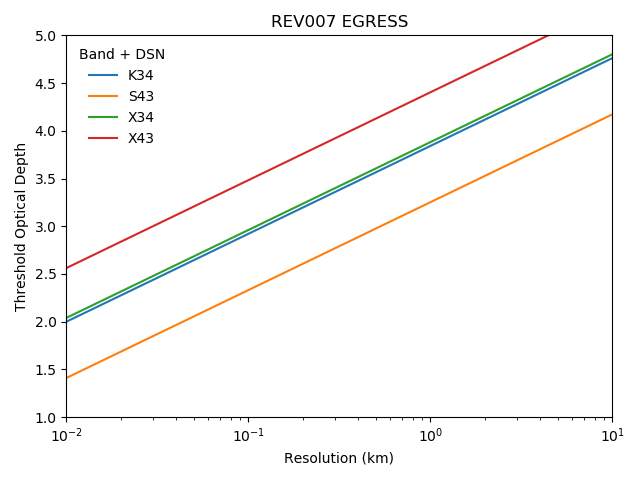
\includegraphics[width=0.48\linewidth]{figs/tauthresh_res_rev007e.png} 
                    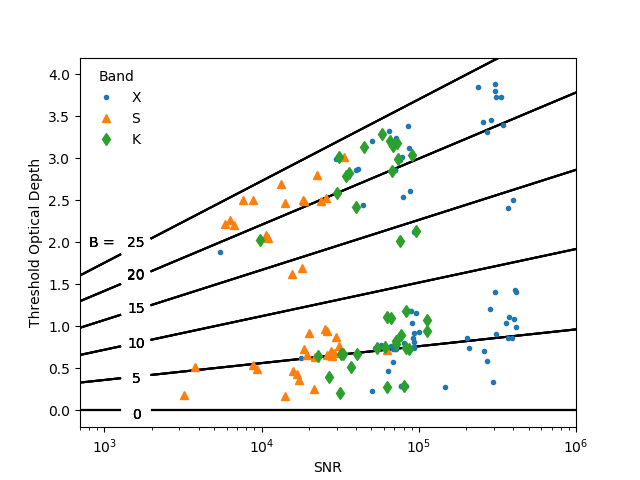
\includegraphics[width=0.505\linewidth]{figs/tauthresh_snr.png}
                    \caption{\textit{Left:} Resolution dependence of $\tau_{TH}$
                            for Rev 007 E. \textit{Right:} Effect of opening angle $B$
                            on $\tau_{TH}$ as a function of $\textrm{SNR}_0$ for
                            $\Delta\rho=0.25$~km. Data are for all 1 kHz files prior to 
                            USO failure}
                    \label{fig:tauthresh}
                \end{figure}
                Following Equations 24-26 in \citet{Marouf1986} and Equations 26
                and 27 in \citet{CRSUG2018}, we compute the threshold optical
                depth using
                \begin{equation}
                    \tau_{TH}=-\sin(|B|)
                    \ln\left[\frac{C_\alpha\dot{\rho}}
                                  {2\mathrm{SNR}_0\Delta\rho}\right]
                \end{equation}
                where $B$ is the ring opening angle and $\dot{\rho}$ is the ring
                intercept radial velocity as computed by and attributed in the
                \texttt{Geometry} class, $C_\alpha=2.41$ is chosen to correspond
                to 70\% confidence\footnote{From \citet{Marouf1986} Equation 25,
                this is given by the root-mean-square of the difference between
                the measured complex signal $X=T+n$ (where $n$ is the additive
                noise from the receiver) and actual complex signal $T$, normalized
                with respect to the expected receiver noise $P_N$.}, and
                $\Delta\rho$ is the radial spacing. For the DLP class, this is
                simply the \texttt{dr\_km} positional argument specified when
                instantiating the DLP class and has a default of 0.25 km. For the
                reconstructed profile, $\Delta\rho$ will depend on the window size
                $W$ and Fresnel scale $F$, the so-called
                \textit{processing resolution} $\Delta R=2F^2/W$. We show the
                dependence of $\tau_{TH}$ on resolution in Figure \ref{fig:tauthresh}
                \citep[cf. Fig. 8,][]{Marouf1986}. Also in Figure \ref{fig:tauthresh} is a demonstration of the effects of both opening angle and SNR on $\tau_{TH}$ for all 1 kHz RSR files prior to USO failure.

        \subsection{Diffraction reconstruction routines}
            \begin{table}[H]
                \centering
                \resizebox{\textwidth}{!}{%
                    \begin{tabular}{l l l}
                        \hline
                        Symbol&Parameter Name&
                        Attribute Name\\
                        \hline
                        $\Delta{R}$&RECONSTRUCTION RESOLUTION (KM)&
                        res\\
                        $\rho$&RING RADIUS&rho\_km\_vals\\
                        $\Delta\rho_{IP}$
                        &RADIUS CORRECTION DUE TO IMPROVED POLE
                        &rho\_corr\_pole\_km\_vals\\
                        $\Delta\rho_{TO}$
                        &RADIUS CORRECTION DUE TO TIMING OFFSET
                        &rho\_corr\_timing\_km\_vals\\
                        $\phi_{RL}$&RING LONGITUDE
                        &phi\_rl\_rad\_vals\\
                        $\phi_{ORA}$&OBSERVED RING AZIMUTH
                        &phi\_rad\_vals\\
                        $\tau$&NORMAL OPTICAL DEPTH&tau\_vals\\
                        $\phi$&PHASE SHIFT&phase\_rad\_vals\\
                        $\tau_{TH}$&NORMAL OPTICAL DEPTH THRESHOLD
                        &tau\_threshold\_vals\\
                        $t_{OET}$&OBSERVED EVENT TIME
                        &t\_oet\_spm\_vals\\
                        $t_{RET}$&RING EVENT TIME&t\_ret\_spm\_vals\\
                        $t_{SET}$&SPACECRAFT EVENT TIME
                        &t\_set\_spm\_vals\\
                        $B$&OBSERVED RING ELEVATION&B\_rad\_vals\\
                        $w$&WINDOW WIDTH FOR RECONSTRUCTION&
                        w\_km\_vals\\
                        $f_{sky}$&SKY FREQUENCY&f\_sky\_hz\_vals\\
                        $F$&FRESNEL SCALE&F\_km\_vals\\
                        $D$&SPACECRAFT-RIP DISTANCE&D\_km\_vals\\
                        $\hat{T}$&DIFFRACTED COMPLEX TRANSMITTANCE&
                        T\_hat\_vals\\
                        $T$&RECONSTRUCTED COMPLEX TRANSMITTANCE&
                        T\_vals\\
                        \hline
                    \end{tabular}
                }
                \caption[Glossary of parameters in TAU file]{%
                    Glossary of parameters contained in
                    RSS\_2005\_123\_X43\_E\_TAU\_01KM.TAB.
                    See companion label
                    (.LBL) files for description of the data.
                }
                \label{tab:easydata_parameters_from_tau_file}
            \end{table}
            All of the diffraction reconstruction tools are located
            within the \texttt{diffrec} subpackage of
            \texttt{rss\_ringoccs}. We include simple tools for
            diffraction reconstruction of the diffraction
            pattern contained in an instance of the \texttt{NormDiff}
            class, as well as more complex tools for modeling problems
            and comparing them with real-world data and geometry.
            The main dependency is the \texttt{numpy} package,
            but some functions also rely on tools found in the
            \texttt{scipy} package. The subpackage is broken into four
            submodules:
            \begin{itemize}[itemsep=0pt]
                \item \texttt{advanced\_tools}
                \item \texttt{diffraction\_correction}
                \item \texttt{special\_functions}
                \item \texttt{window\_functions}
            \end{itemize}
            The \texttt{diffraction\_correction} submodule is the primary
            tool within \texttt{diffrec} and contains the
            \texttt{DiffractionCorrection} class, which is the main utility
            for creating diffraction-reconstructed profiles of radio occultation
            observations. The Python syntax is as follows:
            \begin{lstlisting}[%
                language=python,
                columns=fullflexible,
                gobble=16,
                escapechar=",
                frame=single,
                basicstyle=\footnotesize\ttfamily,
            ]
                In [1]: from rss_ringoccs import diffrec
                In [2]: rec = diffrec.DiffractionCorrection("%
                             "norm_inst, res)
            \end{lstlisting}
            Here, \texttt{norm\_inst} is an instance of the
            \texttt{DiffractionLimitedProfile} class containing the diffracted
            data and \texttt{res} is the user-requested processing
            resolution of the reconstructed profiles in kilometers
            and expressed as a floating point number.
            There are several keywords in this class to allow 
            the user to specify how the diffraction
            reconstruction will be performed.
            \par\hfill\par
            A new feature of \texttt{rss\_ringoccs} is the use of
            special polynomials within the diffraction reconstruction
            steps to greatly reduce computation time without
            sacrificing accuracy. The \textit{Fresnel kernel},
            $\psi(\rho,\rho_{0};\phi,\phi_{0})$, needs to be computed at its
            \textit{stationary} value, $\psi_{s}$:
            \begin{equation}
                \frac{\partial\psi_{s}}{\partial\phi}=0.
            \end{equation}
            We expand $\psi$ in a Taylor expansion about the point
            $\phi_{0}$, and obtain the following:
            \begin{equation}
                \label{eqn:Psi_Taylor_Series}
                \psi=
                    \sum_{n=0}^{\infty}
                    \psi^{(n)}(\rho,\rho_{0};\phi_{0},\phi_{0})
                    \frac{(\phi-\phi_{0})^{n}}{n!}.
            \end{equation}
            The notation $\psi^{(n)}$ represents the
            $n^{\textrm{th}}$ partial derivative of $\psi$ with
            respect to $\phi$. The tuple
            $(\rho,\rho_{0};\phi_{0},\phi_{0})$ is to indicate that
            the coefficients of the Taylor expansion are
            \textit{functions of the other variables},
            and are not constants. We apply Newton-Raphson to find
            the stationary value of $\psi$, and obtain in the first
            perturbation the following value:
            \begin{equation}
                \phi_{s}=
                    \phi_{0}-\frac{\psi'(\rho,\rho_{0};\phi_{0},\phi_{0})}
                                  {\psi''(\rho,\rho_{0};\phi_{0},\phi_{0})},
            \end{equation}
            where, again, derivatives are taken with respect to $\phi$.
            Truncating Eq.~\ref{eqn:Psi_Taylor_Series} at the quadratic term
            and evaluating at $\phi=\phi_{s}$, we obtain:
            \begin{equation}
                \label{eqn:Psi_Approx_Stationary_Value}
                \psi_{s}\approx\psi(\rho,\rho_{0};\phi_{0},\phi_{0})-\frac{1}{2}
                    \frac{\psi'(\rho,\rho_{0};\phi_{0},\phi_{0})^{2}}
                         {\psi''(\rho,\rho_{0};\phi_{0},\phi_{0})}.
            \end{equation}
            The nature of $\psi$ allows the right-hand side of
            Eq.~\ref{eqn:Psi_Approx_Stationary_Value} to be expressed
            exactly in terms of Legendre polynomials. For example, stopping the
            Legendre expansion at the quadratic term gives the classic
            \textit{Fresnel approximation}. This is:
            \begin{equation}
                \psi_{s}=\frac{\pi}{2}\Big(\frac{\rho-\rho_{0}}{F}\Big)^{2}.
            \end{equation}
            We will refer to this approach to the expanson as
            Fresnel-Legendre polynomials.
            \texttt{rss\_ringoccs} allows for several different polynomial
            powers of this expansion by using the \texttt{psitype} keyword.
            This is a \texttt{string}, and the following inputs are allowed:
            \begin{itemize}
                \item `Fresnel' - Classic Fresnel approximation.
                \item `Fresnel3' - Legendre expansion up to the cubic term.
                \item `Fresnel4' - Legendre expansion up to the quartic term.
                \item `Fresnel6' - Legendre expansion up to 6th order.
                \item `Fresnel8' - Legendre expansion up to eighth order.
                \item `Full' - No approximation, Newton-Raphson is applied.
            \end{itemize}
            For all but Rev133, the `Fresnel4' option is more than adequate,
            and can reproduce the PDS results, as well as mimic the results
            obtained by using `Full'. Unless overruled explicitly by the user, `Fresnel4' is the default option. For Rev 133 observations, when the rings were observed nearly edge-on, a known problem with the cubic term of
            $\psi$ persists, and the Fresnel-Legendre polynomials cannot
            adequately capture this. This is in part because the
            Fresnel-Legendre expansion assumes that the first iterate of
            the Newton-Raphson approximation is sufficient, whereas in such
            extreme geometries it is not.
                       \par\hfill\par
            Below is a detailed description of the example 
            included in the \texttt{quick\_look\_run.py} script 
            discussed in Section \ref{sec:quicklook}.
            As with the quick-look
            script itself, this example assumes that
            the user has available the requisite \texttt{*.TAB}
            files generated by the example end-to-end script 
            covered in Section \ref{sec:end2end}.
            The \texttt{ExtractCSVData} 
            class covered in the next section can be used
            to extract information from the \texttt{*.TAB} files and 
            reconstruct the DLP instance \texttt{norm\_inst}.     
            \begin{lstlisting}[%
                language=Python,
                columns=fullflexible,
                basicstyle=\footnotesize\ttfamily,
                frame=single,
                escapechar=',
                gobble=16
            ]
                In [1]: geo = "../Data/GEO.TAB"
                In [2]: cal = "../Data/CAL.TAB"
                In [3]: dlp = "../Data/DLP.TAB"
                In [4]: from rss_ringoccs.tools import ExtractCSVData
                In [5]: from rss_ringoccs import diffrec
                In [6]: norm_inst = ExtractCSVData(geo, cal, '%
                                            'dlp, verbose=False)
                In [7]: tau_inst_f = diffrec.DiffractionCorrection(
                   ...: norm_inst, 1.0, rng="all", psitype="fresnel")
                Computation Time: 12.491324
            \end{lstlisting}
            Note the quite short (12 second) reconstruction time,
            due in part to the
            `Fresnel' setting for psitype and 1 km resolution.
            Running \texttt{DiffractionCorrection}
            with psitype=`full':
            \begin{lstlisting}[%
                language=Python,
                columns=fullflexible,
                basicstyle=\small\ttfamily,
                frame=single,
                gobble=16
            ]
                In [8]: tau_inst_v = diffrec.DiffractionCorrection(
                    data, 1.0, psitype="full", verbose=True)
                    Things print out here...
                Computation Time: 108.427886
                In [9]: tau_inst = diffrec.DiffractionCorrection(
                    data, 1.0, psitype="full")
                Computation Time: 76.470007
            \end{lstlisting}
            \par\hfill\par
            There are several things to note here.
            The computation of $\psi$ is one of the slowest
            parts in the entire diffraction reconstruction
            algorithm. In particular, the computation of the
            \textit{stationary phase} can be quite time-consuming.
            Since `Fresnel' skips all of this, we see a
            substantial reduction in computation time. The data
            set that was used in this example comes from
            the Cassini rev007E occultation observation. We
            can check the validity of Fresnel approximation
            for this set by looking at the difference in the
            two reconstructions. Note that since the power
            is normalized to 1, this is both fractional and
            absolute error:
            \par\hfill\par
            \begin{lstlisting}[%
                language=Python,
                columns=fullflexible,
                basicstyle=\small\ttfamily,
                frame=single,
                escapechar=",
                gobble=16
            ]
                In [10]: import numpy as np
                In [11]: np.max(np.abs(recf.power_vals-rec.power_vals))
                Out[11]: 0.00016784579326811766
                In [12]: "%
                "np.mean(np.abs(recf.power_vals-rec.power_vals))
                Out[12]: 3.5374768401331293e-06
            \end{lstlisting}
            The Fresnel approximation works very well here.
            The default setting of psitype=`Fresnel4'
            is slightly slower than `Fresnel', but still finishes execution
            in less than 20 seconds. For many occultations where
            `Fresnel' fails, `Fresnel4' still produces accurate results.
            Another thing to note is that there is a large
            discrepancy in the computation time for when
            verbose=True and verbose=False is set.
            Since verbose prints out pieces of information for
            every point that is being reconstructed, the
            Python interpreter needs to wait for the line
            to be printed before it can process the next point.
            In most cases this is not an issue, but when speed
            is crucial it may be better to leave verbose set
            to False.
        \subsection{Utility routines}
            Within the \texttt{tools/} subpackage one can find various
            \texttt{pds3\_*\_series.py} scripts and routines
            to read and write PDS3-type data and label files.\footnote{The
            products of these routines have not been thoroughly checked
            for PDS3 compliance.} \texttt{rss\_ringoccs} manages the file
            naming conventions and calling of the
            \texttt{pds3\_*\_series.py} scripts by means of the
            \texttt{write\_output\_files.py} script.
            \par\hfill\par
            Also included as a utility for the quick-look pipeline 
            is the \texttt{ExtractCSVData}, a tool for 
            extracting information from the \texttt{*.TAB} files and 
            reconstructing the DLP instance \texttt{norm\_inst}.
            This can be found in the \texttt{CSV\_tools}
            submodule of the \texttt{tools} subpackage,
            all contained within \texttt{rss\_ringoccs}.
            The steps for importing are shown below.
            \par\hfill\par
            The \texttt{ExtractCSVData} imports user-specified 
            \texttt{*.TAB} files produced by the end-to-end pipeline
            and uses them to construct an instance of the
            \texttt{NormDiff} 
            class that can then be passed on for
            diffraction reconstruction
            as a part of the quick-look process.
            This way, the pipeline only needs to be run once on
            a given data set, and then the user may experiment
            with different resolutions, window functions, etc.,
            on the diffracted data without repeated time
            consuming steps. For example, from the
            master directory of \texttt{rss\_ringoccs}, one could use
            ipython to implement the following to construct a
            \texttt{DiffractionLimitedProfile} instance from \texttt{*.TAB}
            files output from a previous run:
            \clearpage
            \begin{lstlisting}[%
                language=Python,
                columns=fullflexible,
                basicstyle=\footnotesize\ttfamily,
                frame=single,
                escapechar=",
                literate={~}{$\sim$}{1},
                gobble=16
            ]
                cd ~/Research/rss_ringoccs-master
                ipython
                In [1]: path ="%
                "'../output/Rev007/E/Rev007E_RSS_2005_123_X43_E/'
                In [2]: geo = "%
                "path+'RSS_2005_123_X43_E_GEO_20180926_0001.TAB'
                In [3]: cal = "%
                "path+'RSS_2005_123_X43_E_CAL_20180926_0001.TAB'
                In [4]: dlp = "%
                "path+'RSS_2005_123_X43_E_DLP_0100M_20180926_0001.TAB'
                In [5]: from rss_ringoccs.tools.CSV_tools import ExtractCSVData
                In [6]: from rss_ringoccs import diffrec
                In [7]: dlp_inst = ExtractCSVData(geo, cal, "%
                                    "dlp, verbose=True)
                Extracting Data from CSV Files:
                    Extracting Geo Data...
                    Geo Data Complete.
                    Extracting Cal Data...
                    Cal Data Complete.
                    Extracting DLP Data...
                    DLP Data Complete
                    Retrieving Variables...
                    Computing Variables...
                    Interpolating Data...
                    Data Extraction Complete.
                    Writing History...
                    History Complete.
                    Extract CSV Data Complete.
            \end{lstlisting}
            Also note that it is possible to combine \texttt{*.TAB}
            files from different end-to-end runs of
            \texttt{rss\_ringoccs}, which is encouraged for users
            who want to examine the effect different calibration
            inputs might have on the final reconstructed
            optical depth profile.
            \par\hfill\par
            The \texttt{CompareTau} tool, found in the
            \texttt{advanced\_tools} submodule of the
            \texttt{diffrec} subpackage, imports user-specified
            \texttt{*.TAB} files produced by the end-to-end
            pipeline and runs the diffraction reconstruction at
            an additional user-specified spatial resolution for
            the purpose of comparing optical depth profiles for
            the same occultation with the only difference being
            the processing resolution.
            
            \subsubsection{PDS3Reader}
                The \texttt{PDS3Reader} function allows users to easily
                read in a set of PDS3-formatted data and label files without
                having to scroll through and examine a label file in detail
                (for column headers, etc.). To use this function, first verify
                that the desired data and label file are within the same
                directory. Then, follow the example below but replace
                \texttt{lbl\_file} with the path to the desired label file.
                \begin{lstlisting}[%
                            language=Python,
                            basicstyle=\footnotesize\ttfamily,
                            frame=single,
                            escapechar=",
                            columns=fullflexible,
                            literate={~}{$\sim$}{1},
                            gobble=20]
                    ln [1]: import rss_ringoccs as rss
                    ln [2]: lbl_file = 'RSS_2005_123_X43_E_GEO_20180926_0001.LBL' 
                    ln [3]: geo = rss.tools.PDS3Reader(lbl_file, "%
                                                      "use_attr_names=False)
                \end{lstlisting}
                The \texttt{geo} variable will contain two classes as
                attributes: \texttt{series} and \texttt{keywords}.
                \texttt{series} refers to the actual data set, and
                calling \texttt{geo.series.\_\_dict\_\_.keys()} will print
                all the data column headers, as seen in the label file.
                By setting the keyword argument \texttt{use\_attr\_names}
                to \texttt{True}, these column header names will be replaced by
                the attribute name used in \texttt{rss\_ringoccs} to represent
                the same variable (see Tables 5-7). To grab the data associated
                with the column header, simply call \texttt{geo.series.XX},
                where \texttt{XX} is the header name. \texttt{keywords} contains
                all of the keywords listed in the label file, and the
                corresponding keyword values can be called in a similar fashion:
                \texttt{geo.keywords.XX}, where \texttt{XX} is the keyword
                name. Definitions for these keywords can be found in the online
                PDS data dictionary \url{https://pds.nasa.gov/tools/dd-search/}.
                
            \subsubsection{Label history}
            Each label file produced by \texttt{rss\_ringoccs} contains
            a \texttt{PROCESSING\_HISTORY\_TEXT} that lists user information
            (such as Python version, operating system, etc.) as well as an
            accumulated list of all positional and keyword arguments that were
            used to run the pipeline up to part where the label was created.
            Users can visually read this list and rerun the pipeline to
            reconstruct the same profile. Alternatively, users can use the
            \texttt{read\_history} function, which will automatically read
            in the listed inputs and output a requested instance, if available.
            For example, a *TAU.LBL file will contain all of the inputs to the
            \texttt{RSRReader}, \texttt{Geometry}, \texttt{Calibration},
            \texttt{DiffractionLimitedProfile}, and \texttt{DiffractionCorrection}
            classes. Using \texttt{read\_history} on the *TAU.LBL will give users
            the option of returning an instance of any of the above classes.
            % For a *DLP.LBL, users will only be able to reproduce instances
            % up to an instance of the \texttt{DiffractionLimitedProfile} class.
            \par\hfill\par
            This function is useful in particular for those who wish to
            produce a \texttt{dlp\_inst} sampled at finer radial intervals than that in the original DLP file.
            
    \subsubsection{Science tools}
            Some preliminary modeling tools are provided here for use with the data products from \texttt{rss\_ringoccs}. The script \texttt{dtau\_miescatt\_partsize\_grid.py} is one such tool. This script can be run from anywhere in the software directory structure and has no dependencies on other \texttt{rss\_ringoccs} scripts. However, this tool does require the use of an external package, \texttt{PyMieScatt}, which can readily be installed using \texttt{pip} as shown here:
            \begin{lstlisting}[%
                language=bash,
                columns=fullflexible,
                basicstyle=\footnotesize\ttfamily,
                frame=single,
                escapechar=",
                gobble=16]
                pip install pymiescatt
            \end{lstlisting}
            Following \citet{Marouf1983}, this script calculates predictions for observed differential optical depth assuming a power law distribution of particle sizes. Users can specify the ring material index of refraction, range of particle sizes, and power law indices by editing the preamble in the script file. Running the script will output a CSV file and plot, both containing the differential optical depths predicted by Mie scattering physics for the given index of refraction, particle sizes and distributions. These predictions are intended for comparison with differential optical depths calculated from reconstructed normal optical depth profiles output by the \texttt{rss\_ringoccs} pipeline.
     \subsection{Incoherent signal routines}
            All of the routines to produce the incoherent signal results are
            in the \texttt{scatter/} directory in the
            \texttt{rss\_ringoccs} package. One tool performs the STFT spectrogram
            calculations and stacking to improve SNR. The other is a tool
            for users to read in results from the spectrogram output file.
            The \texttt{spectrogram.py} script contains the object class \texttt{Scatter}.
            Instantiating this object requires instances of the RSRReader, Geometry, 
            and Calibration classes. \texttt{Scatter} uses the \texttt{spectrogram} method 
            from the \texttt{scipy.signal} module with a Hamming window to compute 
            the discrete short-time Fourier transform of the phase-corrected complex 
            signal over the entirety of the occultation. Then, its \texttt{stack\_spec}
            method stacks the spectrogram slices to boost the SNR of the incoherent
            signal, which is typically only 1-2 dB above the noise threshold. Following
            rss\_ringoccs file nomenclature, \texttt{Scatter} outputs the spectrogram
            and ancillary information (e.g., radius, frequency, and time dimensions)
            to comma-delimited files.
            We provide the script \texttt{spectro\_reader.py} as a tool for reading the
            output spectrogram and ancillary reference files to build the spectrogram,
            time, frequency, and radius arrays. As a demonstration for reading and visualizing the incoherent signal, we provide an example script \texttt{spectrogram\_plot\_example} in 
            the \texttt{examples} directory that reads in scattered signal data products and 
            normal optical depth profiles from the \texttt{output} directory and plots the results.

    \section{Validation of \texttt{rss\_ringoccs} algorithms}
        In this section, we present tests and validations
        of the performance and output of \texttt{rss\_ringoccs}.
        Perhaps most significantly, this includes a comparison
        of \texttt{rss\_ringoccs} results with those published
        on the PDS as these results were processed using
        state-of-the-art methods following \citet{Marouf1986}.
        This includes a demonstration of the results for
        Cassini and for Voyager, results from raw data sampled
        at different rates, and results from DLPs sampled at
        different rates.
        \subsection{Comparison with results on the PDS}
            \label{sec:pds_valid}
            \subsubsection{Cassini RSS results}
            The results of \texttt{rss\_ringoccs} match those in PDS
            \texttt{CORSS\_8001} extremely well. After completing the Huygens ringlet
            end-to-end example in Section \ref{sec:end2end}, several data products will be created. In 
            Figs.~\ref{fig:rev7ex43_geom_comp_1}-\ref{fig:rev7ex43_geom_comp_2}, we compare our output GEO file, plotted in blue, with the PDS GEO file, plotted in dashed red lines. These values are, for our purposes, essentially the same -- the comparisons without grey dots indicating a fractional error match exactly to the precision listed in the files. 
            \par\hfill\par
            The calibration steps require more complex calculations and some user judgment, but overall the agreement between the calibrated diffraction-limited profiles obtained from \texttt{rss\_ringoccs} and the archived PDS results remains excellent. An important calibration step is to normalize the signal power such that it reaches unity within free-space regions, but the fit type and order rely heavily on user choices. For example, although Figure 9 looks as though the signal power outside of the ring system is at unity, indicating a good fit, if we zoom into a feature and compare our final signal power to that on the PDS, the unity background signals differ slightly. For the examples here, this is seen in the Maxwell ringlet but not the Huygens ringlet. 
              %  Our computation of CAL parameters also, for the most part, match the PDS very well. T
         
            \begin{figure}[H]
                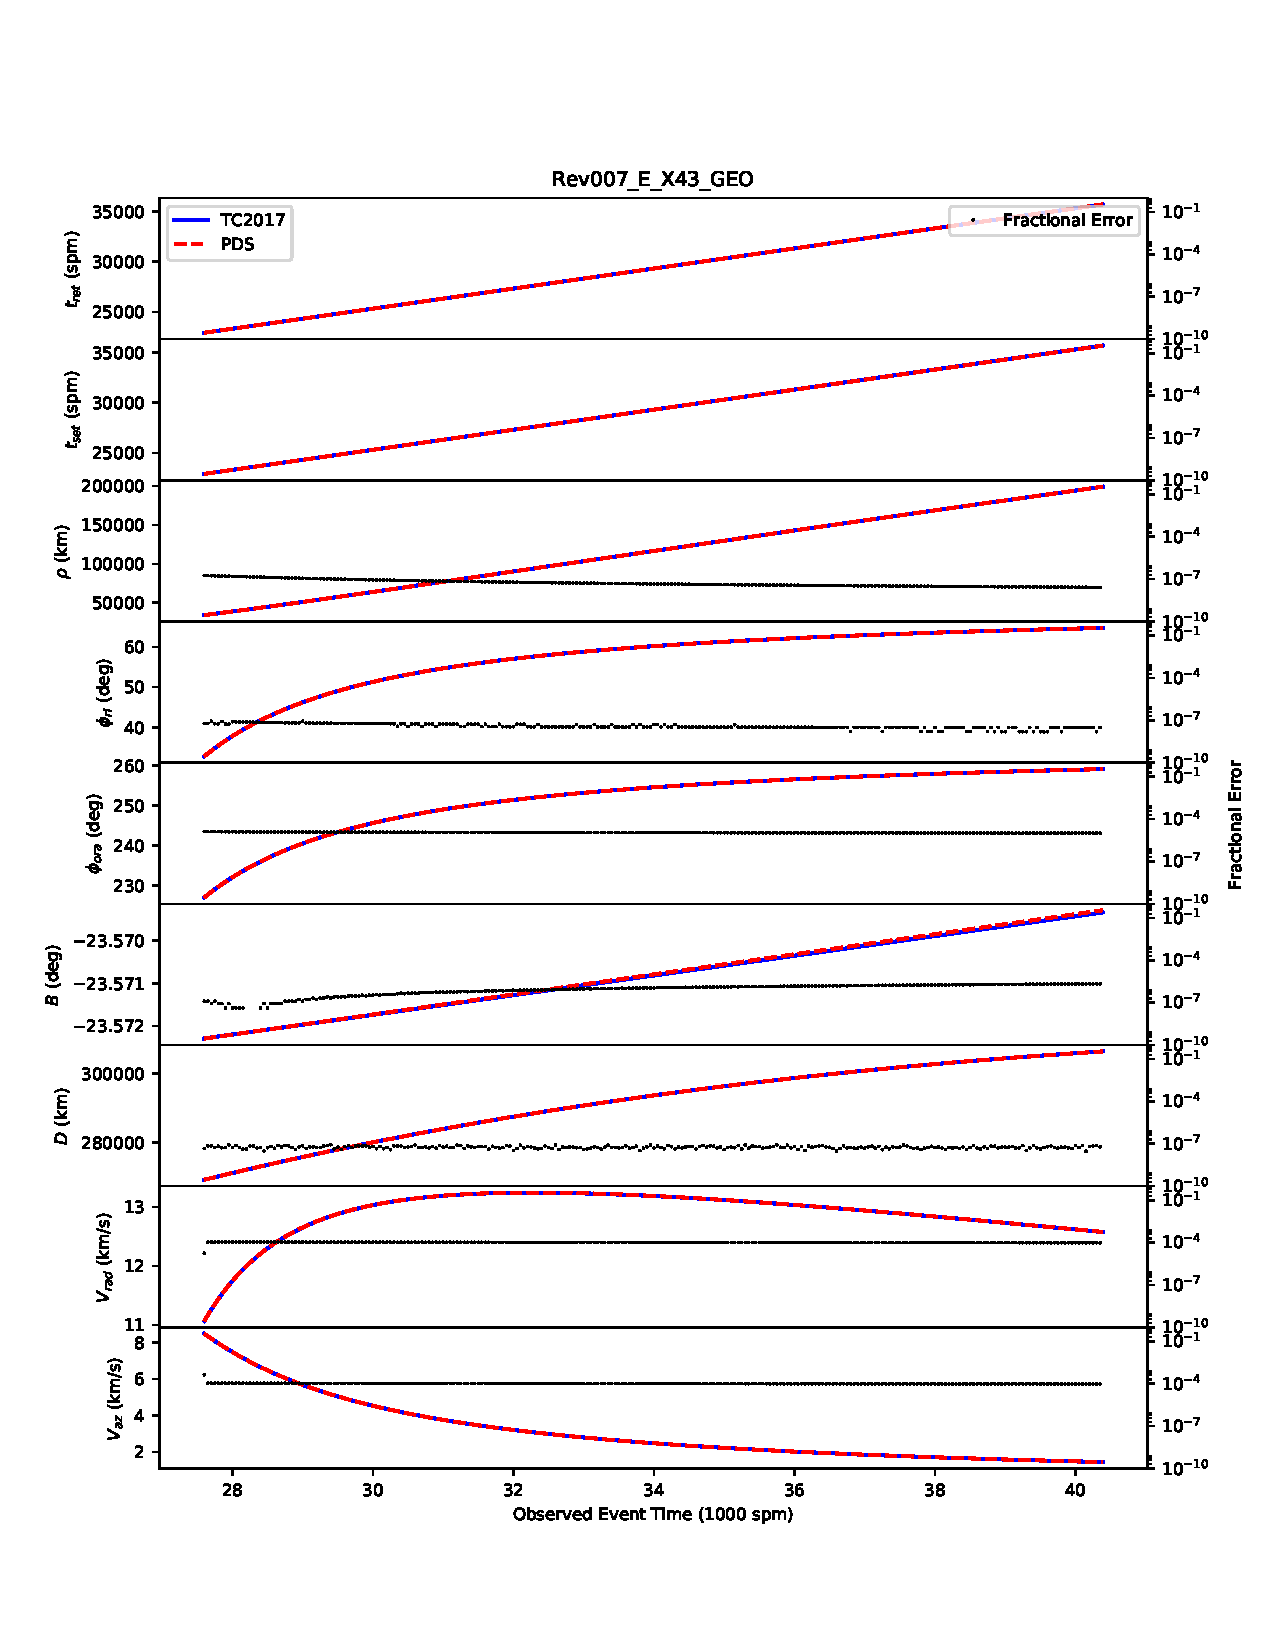
\includegraphics[page=1,width=\textwidth]
                    {figs/Rev007_E_X43_GEO_geom_comp_20190125.pdf}
                \caption[Comparison of geometry parameters for Rev007 Egress X-band.]
                    {Comparison of geometry parameters for Rev007 Egress X-band as viewed
                     from DSS-43. PDS \texttt{CORSS\_8001} data product
                     \texttt{Rev007/Rev007E/Rev007E\_RSS\_2005\_123\_X43\_E/RSS\_2005\_123\_X43\_E\_GEO.TAB}
                     values are plotted in dashed red lines, with \texttt{rss\_ringoccs} values
                     overplotted in blue. Fractional error between the two are plotted
                     on the right-hand y-axis in grey dots.}
                \label{fig:rev7ex43_geom_comp_1}
            \end{figure}
            \begin{figure}[H]
                \includegraphics[page=2,width=\textwidth]
                    {Rev007_E_X43_GEO_geom_comp_20190125}
                \caption[More comparisons of Rev007 geometry.]
                    {Comparison of geometry parameters for Rev007 Egress X-band as
                     viewed from DSS-43. PDS \texttt{CORSS\_8001} data product
                     \texttt{Rev007/Rev007E/Rev007E\_RSS\_2005\_123\_X43\_E/RSS\_2005\_123\_X43\_E\_GEO.TAB}
                     values are plotted in dashed red lines, with \texttt{rss\_ringoccs}
                     values overplotted in blue. Fractional error between the two are
                     plotted on the right-hand y-axis in grey dots.}
                \label{fig:rev7ex43_geom_comp_2}
            \end{figure}
            \clearpage
            \begin{figure}[H]
                \centering
                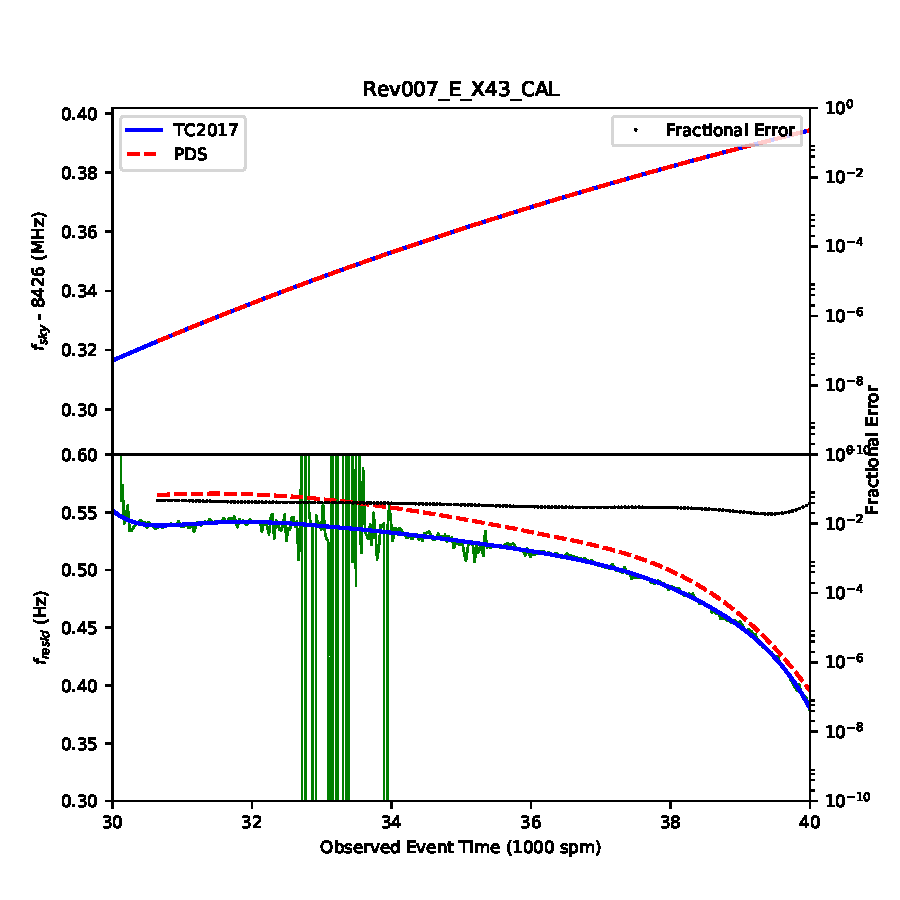
\includegraphics[width=\textwidth]
                    {Rev007_E_X43_CAL_cal_comp_20190128.pdf}
                \caption[Comparison of Frequency Offset with PDS]
                    {Comparison of the Frequency Offset and Residual Frequency
                     computed for the Rev007 E X43 data set.}
                \label{fig:rev7ex43_cal_comp_1}
            \end{figure}
            If Fig.~\ref{fig:rev7ex43_cal_comp_1} we plot the output of the
            calibration steps of the pipeline for the Rev007 E X43 data set.
            Plotted with this are the results found on the PDS, as well as the
            fractional error between the two. Below in
            Fig.~\ref{fig:rev7ex43_pnorm} we plot the raw power that is
            extracted from the RSR files:
            \clearpage
            \begin{figure}[H]
                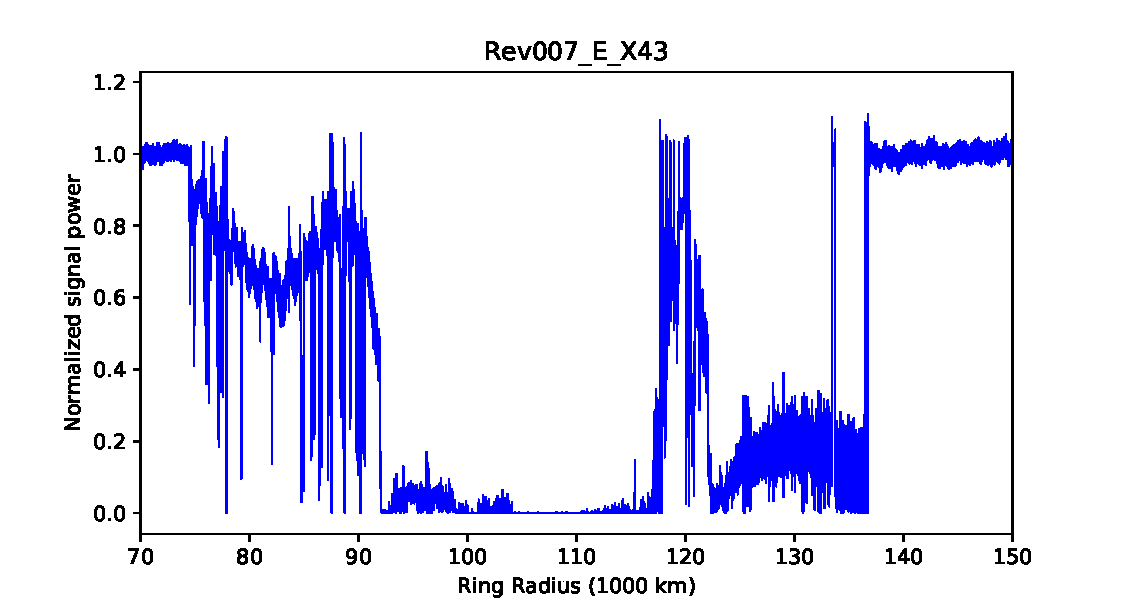
\includegraphics[page=1,width=\textwidth]
                    {Rev007_E_X43_PNORM_20190128.pdf}
                \caption{Raw Power from Rev007 E X43}
                \label{fig:rev7ex43_pnorm}
            \end{figure}
            Finally, at the end of the pipeline we obtain the reconstructed
            profiles of the Saturnian ring system. It is important to note that
            the normalization step can be very subtle. As an example of this,
            we show the reconstruction of Rev007 E X43 in
            Fig~\ref{fig:rev7ex43_huygens_comp} about the Huygens ringlet and
            the Maxwell ringlet. The default fit was used to create the
            normalized power. The fit and reconstruction worked extremely well
            for Huygens, but there is a slight discrepancy for the Maxwell
            ringlet. Adjusting the polynomials used in the spline fit will
            alleviate this error, and it is up to the user to decide when the
            fit is sufficient for their needs.
            \begin{figure}[H]
                \centering
                \begin{subfigure}[b]{0.49\textwidth}
                    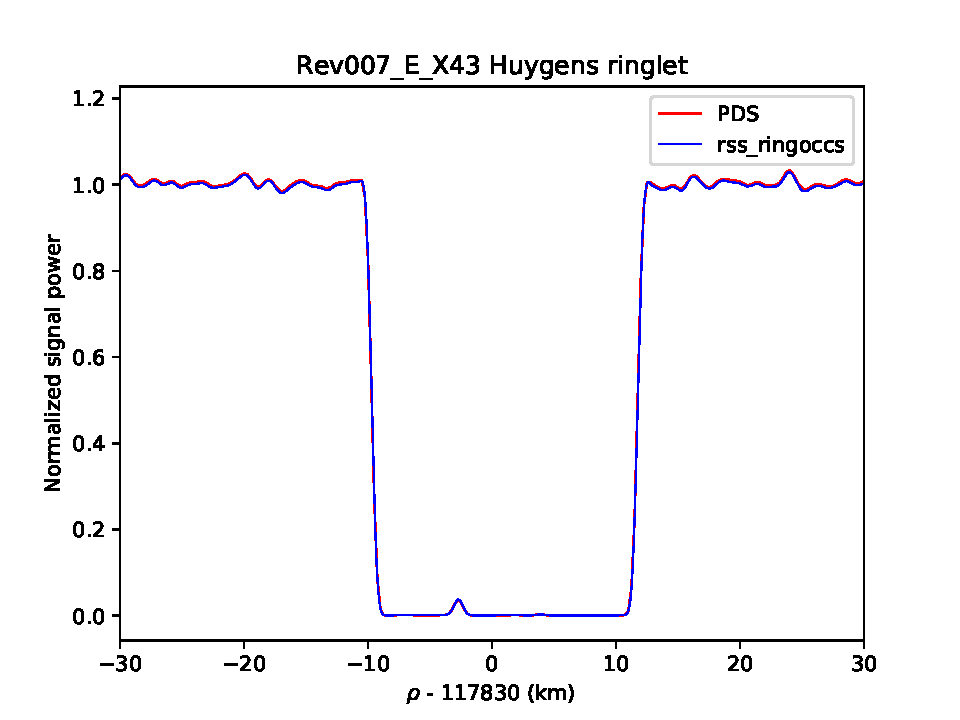
\includegraphics[width=\textwidth]
                        {Rev007_E_X43_PNORM_Huygens_comp_20190128.pdf}
                    \subcaption{Huygens ringlet reconstructed normalized power.}
                \end{subfigure}
                \begin{subfigure}[b]{0.49\textwidth}
                    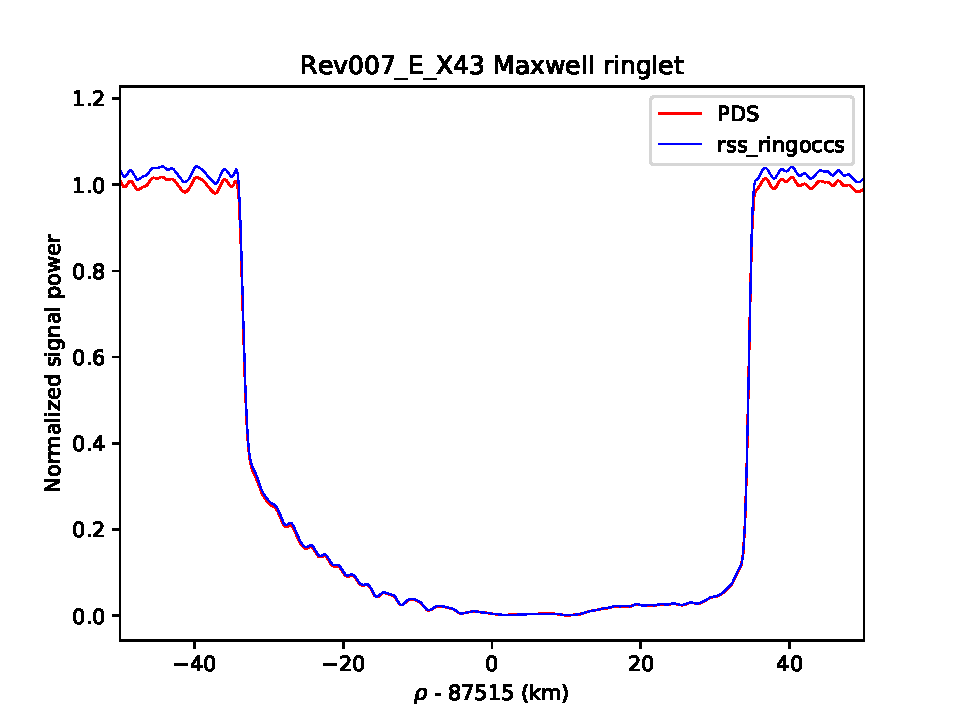
\includegraphics[width=\textwidth]
                        {Rev007_E_X43_PNORM_Maxwell_comp_20190128.pdf}
                    \subcaption{Maxwell ringlet reconstructed normalized power.}
                \end{subfigure}
                \caption[Comparison of Reconstructed Power]
                        {Comparison of reconstructed normalized power
                         with PDS results. PDS results are plotted in
                         \textcolor{red}{red} and can be found from
                         \texttt{Rev007/Rev007E/Rev007E\_RSS\_2005\_123\_X43\_E/RSS\_2005\_123\_X43\_E\_TAU\_01KM.TAB}).
                         \texttt{rss\_ringoccs} results are in
                         \textcolor{blue}{blue}.}
                \hfill
                \label{fig:rev7ex43_huygens_comp}
            \end{figure}
        \subsection{Effect of different sampling rates}
            The raw data recorded at the DSN stations are sampled
            at 16 kHz. The high resolution of these data poses two
            difficulties: (i) each RSR data file is at least many
            hundreds of MB in size for an ingress or egress
            diametric occultation (chord occultations are even larger),
            which can be cumbersome especially for users downloading a
            large number of RSR files; (ii) the \texttt{rss\_ringoccs}
            processing time on a conventional laptop for each data
            file can be at least thirty minutes for diametric
            occultation (even longer for chord occultations), which
            is particularly computationally expensive for users
            planning to reduce data for numerous occultations. The
            PDS provides RSR data files with the raw data down-sampled
            to 1 kHz. These files are twelve to sixteen times smaller
            (lower limit of tens of MB instead of hundreds)
            and take 90 to 180 seconds for \texttt{rss\_ringoccs} to process.
            \par\hfill\par
            The computational benefits of utilizing the 1 kHz files
            over the 16 kHz files is clear. However, we must demonstrate
            that the down-sampled data yield results comparable to
            those of the raw high-resolution data. To begin this
            validation, we process 1 kHz and 16 kHz data files for
            X band at high ring opening angle ($B\approx23^\circ$)
            and Ka band at low ring opening angle ($B\approx5^\circ$).
            Then, we compare and contrast the 1 kHz and 16 kHz
            processing results from the calibration, DLP, and
            reconstruction steps as shown in Fig.~\ref{fig:1vs16khz} at the end of this 
            document.
            \par\hfill\par
            \begin{figure}[!ht]
                \centering
                \begin{subfigure}[b]{0.94\textwidth}
                    \includegraphics[width=0.49\textwidth]
                        {figs/validation/%
                         Rev007E_RSS_2005_123_X43_E_fresidfit_comp.png}
                    \includegraphics[width=0.49\textwidth]
                        {figs/validation/%
                         Rev125E_RSS_2010_027_K55_E_fresidfit_comp.png}
                    \subcaption{Ratio of 1 kHz to 16 kHz Frequency Offset
                                Residual Fits.}
                \end{subfigure}
                \hfill
                \begin{subfigure}[b]{0.94\textwidth}
                    \includegraphics[width=0.49\textwidth]
                        {figs/validation/%
                         Rev007E_RSS_2005_123_X43_E_powernorm_comp.png}
                    \includegraphics[width=0.49\textwidth]
                        {figs/validation/%
                         Rev125E_RSS_2010_027_K55_E_powernorm_comp.png}
                    \subcaption{Ration of 1 kHz to 16 kHz Free Space Power Fits.}
                \end{subfigure}
                \hfill
                \begin{subfigure}[b]{0.94\textwidth}
                    \includegraphics[width=0.49\textwidth]
                        {figs/validation/%
                         Rev007E_RSS_2005_123_X43_E_dlptau_comp.png}
                    \includegraphics[width=0.49\textwidth]
                        {figs/validation/%
                         Rev125E_RSS_2010_027_K55_E_dlptau_comp.png}
                    \subcaption{Difference between 1 kHz and 16 kHz
                                DLP optical depths.}
                \end{subfigure}
                \hfill
                \begin{subfigure}[b]{0.94\textwidth}
                    \includegraphics[width=0.49\textwidth]
                        {figs/validation/%
                         Rev007E_RSS_2005_123_X43_E_rectau_comp.png}
                    \includegraphics[width=0.49\textwidth]
                        {figs/validation/%
                         Rev125E_RSS_2010_027_K55_E_rectau_comp.png}
                \end{subfigure}
                \caption{Validation of 1 kHz processing using raw 16 kHz
                         processing for Rev 007 E X band and Rev 125 E Ka band.}
                \label{fig:1vs16khz}
            \end{figure}
           % \par\hfill\par
            The frequency offset and freespace power
            fits differ by less than 0.1\% within the ring system,
            while the computed frequency offsets differ by less
            than 0.01\%. The DLP optical depth values are typically
            within 0.01 dB of one another, although this is not
            the case for the part of the profile associated with the
            B ring. Any differences seen between the two profiles
            can be ascribed to changes in the diffraction pattern
            when the profile is down-sampled to the DLP radial
            sampling resolution. This assertion is substantiated
            by the similarity of the diffraction-corrected optical
            depth profiles. Because the diffraction reconstruction
            eliminates diffraction patterns in the profile, the
            excellent agreement of the two reconstructed profiles
            indicates that the disparity between the DLP optical
            depths is due to differences in the diffraction patterns.
            \par\hfill\par
            Having been demonstrated to yield results comparable
            to those from the 16 kHz files for 1 km reconstructions, the 1 kHz files are
            recommended for processing instead of the 16 kHz files.
            Users can obtain 1 kHz files for the majority of
            occultations from the PDS with only a few exceptions.
            In these cases, we recommend the user decimate the 16
            kHz file to 1 kHz at the start of the pipeline by
            setting the \texttt{decimate\_16khz\_to\_1khz}
            keyword argument equal to \texttt{True}.
            
            \section{Voyager 2 Uranus occultation}
            The Voyager 2 X-band (3.6 cm) radio occultation of the Uranian rings on
            January 24-25, 1986 provides the highest resolution observations for the
            Uranian ring system to date. Definitive analysis of the Voyager 2 occultation
            was performed by \citet{Gresh1989} and the final results were archived
            at 50~m resolution. The best Earth-based Uranus ring occultation
            dataare diffraction-limited to 1-2
            km, inhibiting detailed analysis of internal structure of the rings. The Voyager 2 RSS Uranus ring occultation
            SNR is high enough to push the diffraction-reconstructed resolution to 20~m to reveal more internal
            structure of the rings, opening up possibilities for new
            science. These observations provide a unique opportunity to demonstrate the applicability of the \texttt{rss\_ringoccs} reconstruction software to contexts outside of the Cassini radio occultations of Saturn's rings with readily-available validation of the results.
            \subsection{Changes to the procedure}
            While the procedure for processing the Voyager 2 radio occultation data is comparable 
            to the approach taken by \texttt{rss\_ringoccs} for the Cassini radio occultations, 
            there are some key differences that required adapting some components of the default processing pipeline.
            \begin{enumerate}
                \item Voyager 2 RSS Uranus ring  data are stored in binary files that are not formatted in the same manner 
                as the RSR files for Cassini radio occultations stored on the PDS. This requires a 
                unique file reader.
                \item The imaginary component of the complex signal was not recorded and must be 
                inferred from the real component.
                \item The Uranian ring system is highly inclined with respect to the Earth. While enabling the high SNR 
                necessary for high-resolution reconstruction, this changes the occultation geometry.
                \item Each ring of Uranus has a different inclination and eccentricity, which 
                requires separate treatment of the occultation geometry for each ring to 
                accurately calculate the ring intercept radius in each ring frame (for the 
                Saturnian rings, \texttt{rss\_ringoccs} computes the geometry for Saturn's 
                equatorial reference frame). This requires processing each ring individually.
                \item The oscillator on board the Voyager 2 spacecraft did not possess the same 
                quality or precision as the USO on board the Cassini spacecraft. This requires 
                adjustments to the phase corrections using the frequency offset, as well as an 
                additional step in detrending the systematic drift in signal phase.
                \item Each ring is accompanied in both radial directions by substantial amount of 
                free space power, which eliminates the need for gap finding but does require locally fitting for the 
                free space power in the vicinity of each narrow ring.
                \item Output file documentation, i.e., the LBL files, must be adapted to reflect the 
                occultation observation information and processing history.
                %\item \citet{Gresh1989} suggests a cant angle and elliptical geometry both affect 
                %the reconstruction of the original profiles from the DLPs.
            \end{enumerate}
            We provide an adaptation of our software with the v1.2 release of \texttt{rss\_ringoccs} 
            that addresses the majority of these issues.
             \par\hfill\par
            \subsubsection{Changes to reading raw data}
            The original Voyager 2 RSS Uranus ring occultation observations at X-band were recorded at 50 kHz on digital tapes when received by the 
            DSN stations in Parkes and Canberra. They are not currently available on the PDS, but Dick Simpson (NASA/PDS) kindly transferred these data to CDs, and then to 
            DVDs, which he provided to our team. To obtain the raw X-band data files that contain the Uranus ring events, submit a request to Dick French, reachable at rfrench@wellesley.edu.
            \par\hfill\par
            We have designed an object class that, when 
            instantiated, reads in the Voyger 2 RSS binary files from the local drive. 
            The raw data contain only the real part of the complex transmittance. 
            To recover the complete complex signal, the 
            Uranus file reader class uses a Hilbert transform to compute $Q$ from the real component 
            $I$ stored in the binary file.
           \subsubsection{Changes to geometry}
           The \texttt{Geometry} class continues to utilize \texttt{spiceypy}; however, this requires 
           a different set of the kernel reference files to compute the occultation geometry. Most of 
           these kernel files are provided with the v1.2 release. Those not included are large 
           ($>100$ Mb) and are also not available from the PDS. These kernel files are available upon 
           request from Dick French, reachable at rfrench@wellesley.edu. 
           \par\hfill\par
           What distinguishes the Uranus version
           of \texttt{Geometry} from that of \texttt{rss\_ringoccs} is its processing of the
           occultation geometry for each ring in its own reference frame rather than the
           host planet's equatorial reference frame. The frame kernel for each ring accounts for the ring's inclination and nodal regression. This enables more accurate calculation of the ring
           intercept radius.
           %%%
           \subsubsection{Changes to calibration}
           Modifications to the \texttt{Calibration} step to accommodate Voyager 2 Uranus RSS observations involved two components of the phase corrections. The
           frequency offset correction original to \texttt{rss\_ringoccs} is estimated assuming that the
           frequency offset falls in a 300 Hz window centered on 0 Hz with 0.5 Hz resolution in the
           discrete Fourier transform. For the Voyager 2 Uranus ring occultation, the frequency offset drifts
           over a 500 Hz window centered on -11 kHz. Additionally, the ring locations can be
           calculated from pre-existing orbital parameters, allowing us to mask the frequency offset
           to exclude any effects of the rings on the computed frequency offset from the fit to the
           frequency offset. Fitting the frequency offset is done before processing each individual
           ring because the frequency offset is not ring specific. Fitting the frequency offset
           could not be done with a single polynomial because of a cusp that occurs in both the
           ingress and egress occultations. Our solution to this was to split the frequency offset
           data into two sets where the cusp occurs in SPM and fit each set separately. While 
           \citet{Gresh1989} fit each set of frequency offset values with a second order polynomial, 
           we find the frequency offset is better described by a ninth order polynomial.
           \par\hfill\par
           Each ring is then corrected by means of the phase detrending function as described in \S\ref{sec:calroutines}.
           The oscillator on board Voyager 2 was not as stable as the USO on Cassini, 
           and the default first-order phase correction used in \texttt{rss\_ringoccs} is not 
           sufficient. After each ring undergoes first-order phase correction and downsampling to 5 kHz
           (necessary for the desired 5 m DLP resolution for the Uranian rings), an additional phase
           correction is applied. First the phase is unwrapped to recover the phase drift. Due to
           noise and diffraction patterns present in the signal phase, the unwrapping is not always
           successful. Corrections to the phase unwrapping are made using parameters stored in an
           ancillary reference file \texttt{phase\_unwrap\_params.py}. We do not recommend that users add 
           to, remove, or otherwise change these parameters, but users may do so at their own risk. 
           \par\hfill\par
           Once the unwrapping corrections are made, we convolve the unwrapped phase by 
           with a 1 second boxcar kernel. This time-averaging is comparable to the \citet{Gresh1989}
           approach of applying a low-pass filter to the unwrapped phase to obtain a fit to the regional drift in phase. Unlike
           the low-pass filter approach, our time-averaging does not fully preserve the diffraction
           pattern encoded in phase after subtracting the fit from the observed phase. This poses a
           problem because this diffraction pattern is necessary for reconstructing the original profile. To
           preserve the diffraction pattern, we fit a second-order polynomial to the time-averaged
           unwrapped phase adjacent to the ring profile (where the diffraction pattern occurs in the
           phase) and replace the time-averaged fit over the diffraction pattern with the polynomial 
           estimate, effectively assuming the polynomial is characteristic of the phase drift present in 
           the diffraction pattern. Finally, we subtract the total fit from the unwrapped phase to correct
           for the second-order drift. This produces phase profiles comparable to those shown in \citet{Gresh1989}.
           \par\hfill\par
           During our preliminary processing of the Voyager 2 data, we found that normalizing the power
           before resampling to radius (the default sequence in \texttt{rss\_ringoccs} would sometimes result in an
           average normalized free space power other than unity. Performing the power normalization
           after resampling the data from observed event time to ring intercept radius eliminates this
           effect. After resampling the data to uniform sampling in radius, we mask out each ring region
           identified by orbital parameters along with an additional 15 km on either side of the profile
           to exclude the entire diffraction pattern from the fit. Then, we fit the free space power with
           a ninth order polynomial and divide the total diffraction-limited power by the fit to obtain
           the normalized diffraction-limited profile.
           %%%
           \subsubsection{Changes to DLP}
           As in \texttt{rss\_ringoccs}, the DLP step primarily entails interpolating the Geometry and
           Calibration results to the uniform sampling in ring intercept radius. Threshold optical depth is
           calculated using noise power estimated from the STFT of the phase-corrected freespace power. 
           Then, the reconstruction window size is estimated for the highest reconstruction resolution (20 m in this case) and Fresnel scale calculated by Geometry. To ensure reconstruction of the total ring profile with several kilometers of baseline freespace on either side of the profile, we pad the ring DLP profile output with additional data on either side of the profile to account for the  window size necessary for reconstructing the end points. Limiting output to this small range of profile power dramatically reduces processing time as well as the output file size.
           %%%
           \subsubsection{Changes to diffraction reconstruction}
           The reconstruction routines remain unchanged from the v1.2 \texttt{rss\_ringoccs} version of diffrec. The major differences are in the default inputs for calling the \texttt{DiffractionCorrection}. The \texttt{res\_fac} is set to unity so that the reconstruction and processing resolutions are identical, consistent with the MTR86 approach used by \citet{Gresh1989}. The Allan deviation is set to the $2\times10^{-13}$ value suggested by \citet{Gresh1989}. The default processing window is set to a Kaiser-Bessel window with $\alpha=2.5$.
           \subsection{Validation of Uranus processing}
           To validate our processing results, we compare ring reconstruction at 50 m to the 50 m 
           reconstructions computed and archived by \citet{Gresh1989}. In general, the diffraction-reconstructed ring profiles are in excellent agreement in detailed structure, effective resolution, and even in the patterns of the free-space noise. We consider this to be a
           successful validation of our method for processing the raw Voyager 2 data. Thus, our
           reconstruction of the raw Voyager 2 data can be considered comparable to that of
           \citet{Gresh1989} and can be reliably used to produced profiles at higher resolutions.
           \begin{figure}[H]
            \centering
            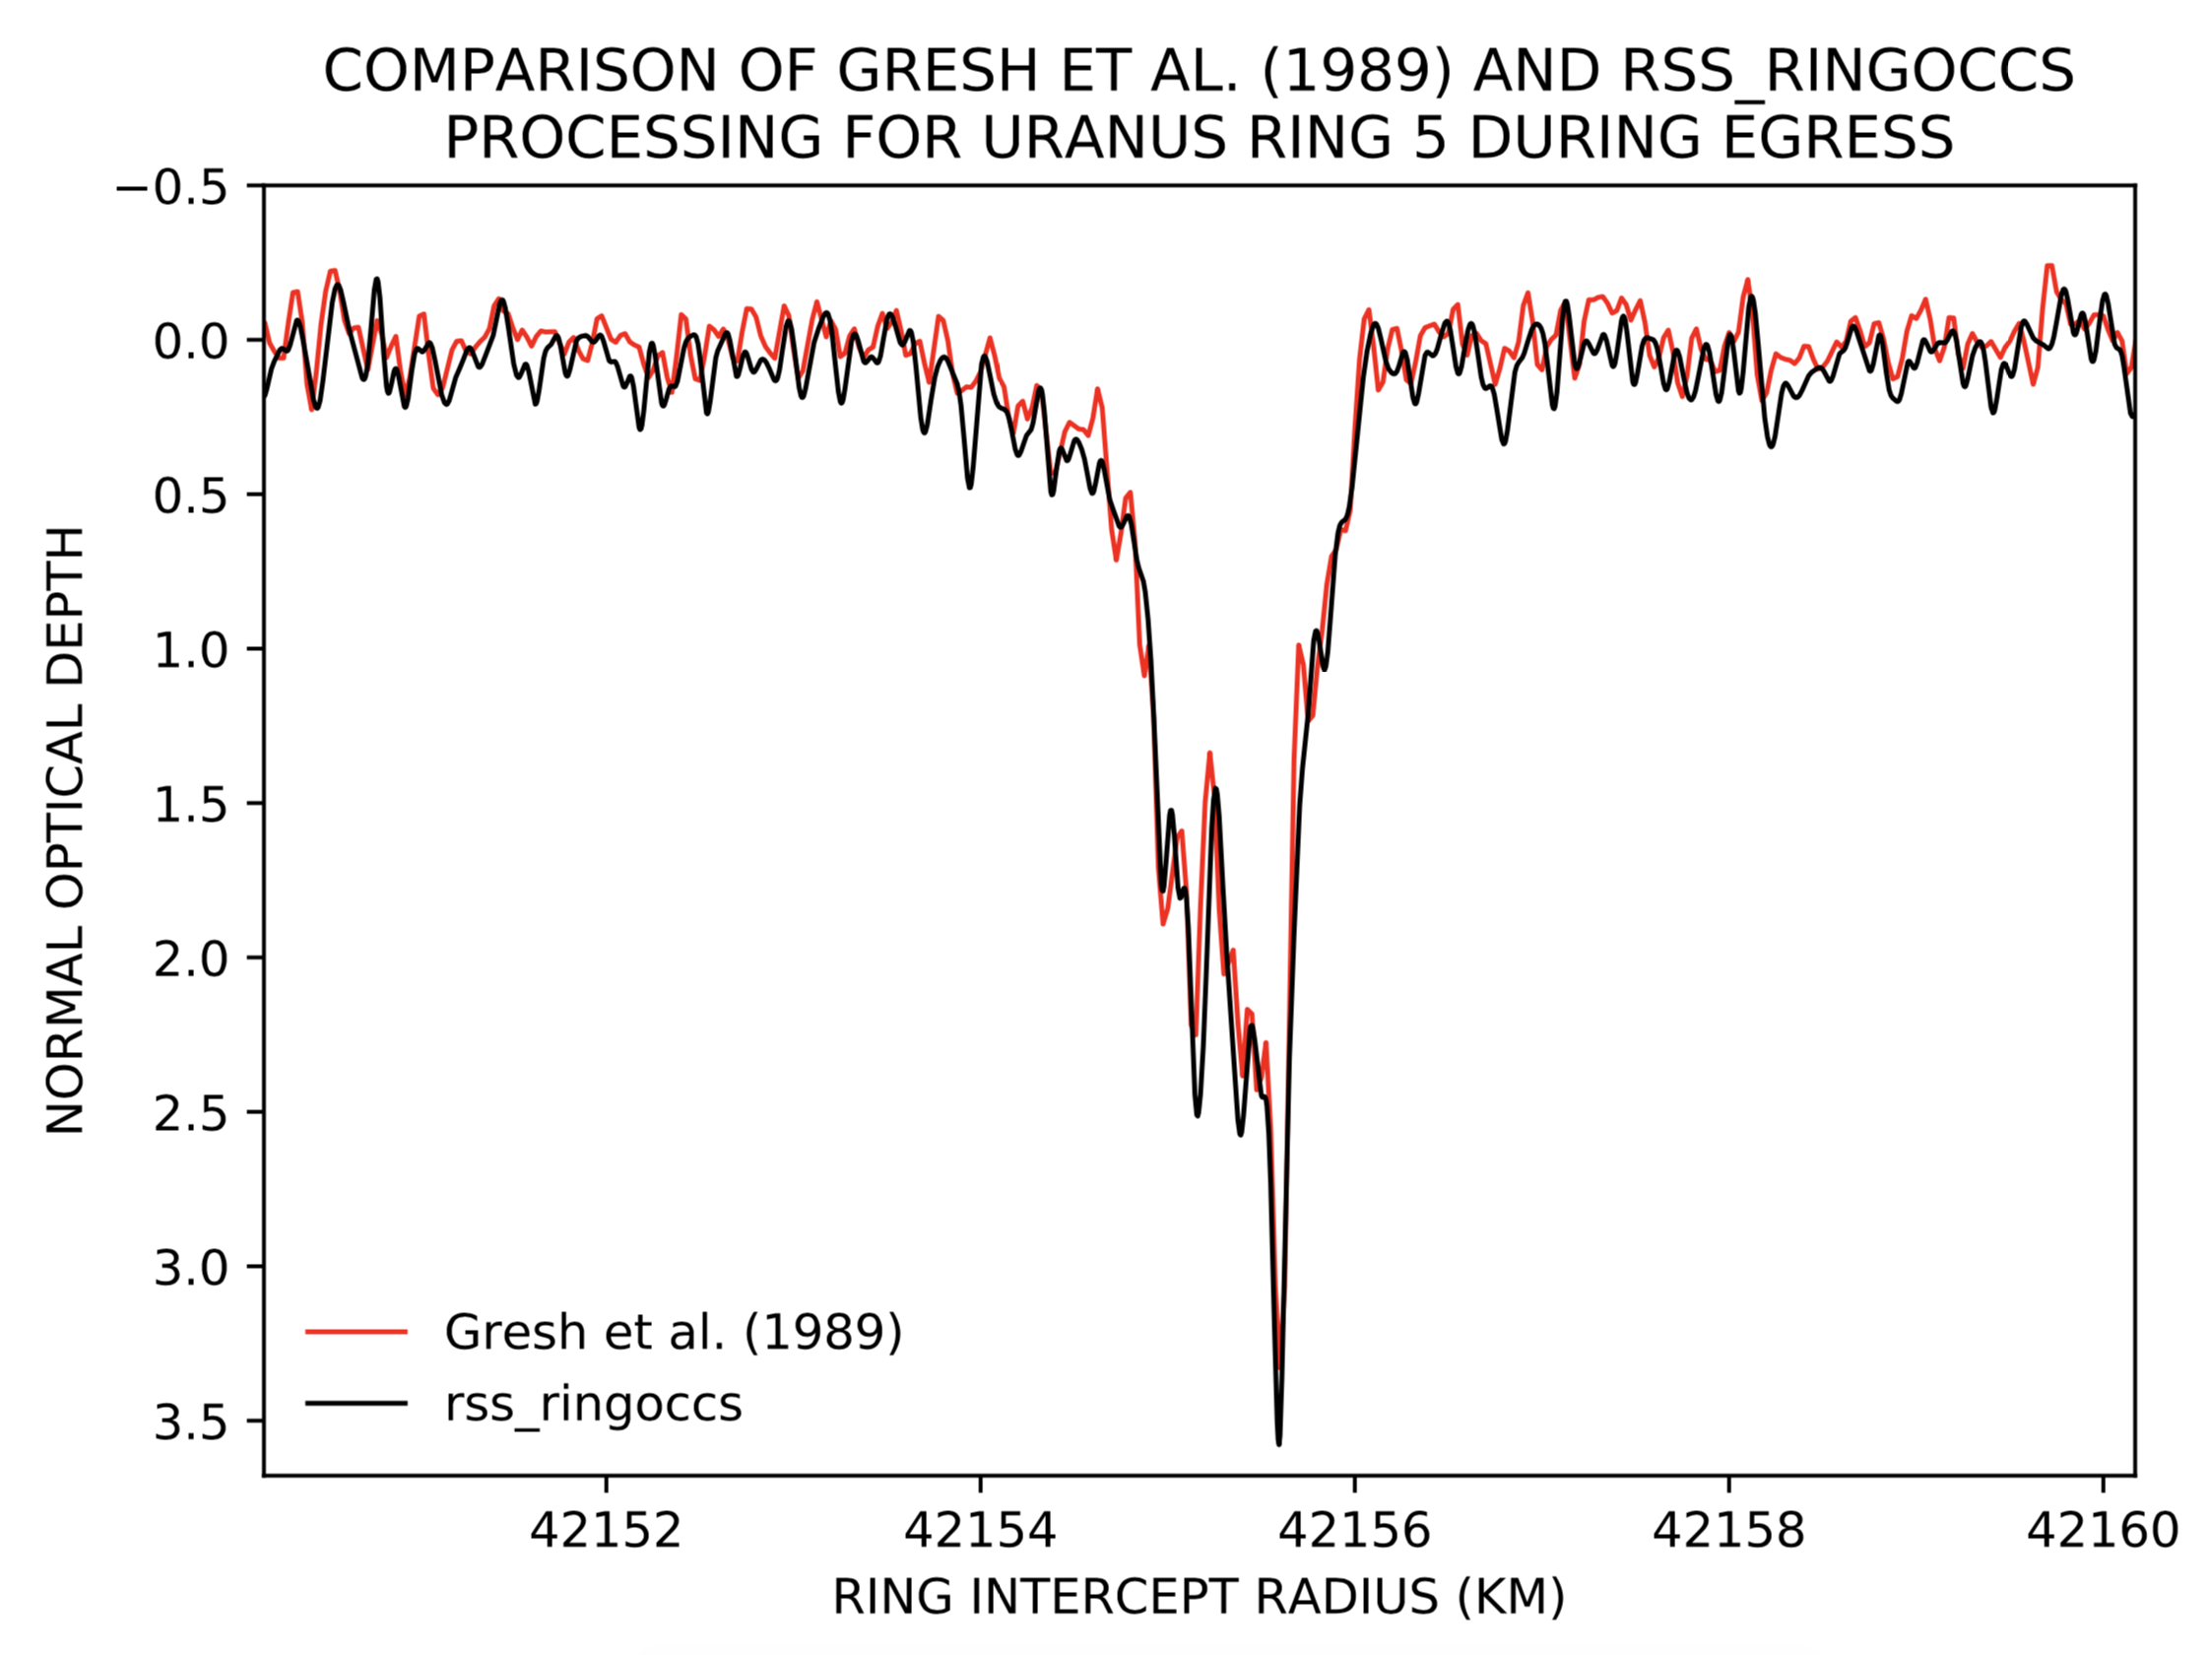
\includegraphics[width=0.75\linewidth]{figs/GRESH_E5_COMPARE.png}
            \caption{Comparison of our adapted \texttt{rss\_ringoccs} processing of the Voyager 2 Uranus ring 5 egress occultation with that of \citet{Gresh1989}.}
           \end{figure}
           Any disagreement between the \citet{Gresh1989} profiles and ours is small and could
           be attributed to several systemic differences. For example, \citet{Gresh1989} may not have
           recovered the imaginary component of the complex signal in the same manner as our
           pipeline. Their approach to phase corrections differs from ours and required three
           separate steps rather than two. It is also not explicitly clear which window function was used by 
           \citet{Gresh1989} for their reconstruction. Finally, as of V1.2, our pipeline 
           does not yet account for a elliptical ring geometry or a cant angle during the reconstruction.
    \section{Where to go from here}
        \subsection{The Cassini RSS data catalog}
            We have created a \texttt{CSV} file (\texttt{data\_catalog\_V180806.csv}, located within
            the \texttt{tables} directory, listing all 1 kHz Cassini
            ring occultation RSR files available on the PDS.
            This catalog includes information of each RSR
            file, such as wavelength/frequency band, observing
            station information, sampling rate, associated
            kernels, etc., as well as relevant geometry parameters
            that can help users determine which file they want
            to use. The column headers and definitions for this
            catalog are also available within the
            \texttt{tables} directory in \texttt{data\_catalog\_definitions\_V180806.txt}.
        \subsection{Selecting an RSR file to process}
            \label{choose_rsr}
            Before using \texttt{rss\_ringoccs}, we recommend users
            browse the Cassini RSS data catalog to find an appropriate
            RSR file to process. Factors such as elevation angle,
            antenna size, ring radius range covered by the occultation, and ring opening angle can
            affect this decision. 
            \par\hfill\par
            First, users should establish that the RSR file covers
            the radius range of interest. Some occultations, such
            as chords, do not cover the entire ring system
            (see Figure \ref{fig:rev54}). Next, depending on the
            research goal, users should select an observation with
            the desired ring opening angle. For high optical depth structure, a large 
            ring opening angle is generally desirable, since it minimizes the slant
            path optical depth, whereas low ring opening angles are preferable for detecting vertical structure in the rings and probing tenuous material. Another
            factor to consider is the Earth receiving station.
            Different stations will record in different bands
            (S-, X-, or Ka-band) using different sized antennas
            (34~m or 70~m), affecting the SNR. The location of the DSN is also important,
            as Cassini could be lower in the sky when observed from one station
            than another -- this affects the
            amount of atmosphere the signal must go through to reach
            the station. These station-related factors can affect
            the overall SNR as well as the background power drift.
        \subsection{Choosing a radial resolution}
            As discussed in Section~\ref{sec:resolutions},
            users must specify a desired radial resolution to \texttt{rss\_ringoccs}
            in the form of radial sample spacing in km for both the DLP and
            the reconstructed profile. The latter must always be at least
            8/3 greater than the former; however, there are additional
            considerations in choosing a sample spacing.
            \par\hfill\par 
            In Figure 8, \citet{Marouf1986} show a relation between threshold 
            optical depth $\tau_{TH}$ (Section~\ref{sec:tauthresh}) and processing
            resolution $\Delta R$ for X and S band. Because lower resolutions 
            lead to larger SNR values, $\tau_{TH}$ increases with $\Delta R$. 
            If the intrinsic SNR is low--more often the case in Ka band or
            low-elevation observations with large Earth atmosphere extinction--
            a small radial sampling rate might not produce meaningful results
            because the profile normal optical depth frequently exceeds the 
            threshold optical depth. In such cases, we recommend that users consider
            the threshold optical depth when specifying a desired resolution.
        \subsection{Execution time benchmarks}
            %\textbf{Need to update this section.}
            The single-file end-to-end example script discussed in 
            \S\ref{sec:end2end} includes a benchmark computation time for a
            typical 1 kHz RSR file for a diametric occultation. When run,
            \texttt{e2e\_run.py} will print out the expected processing time
            for a single 1 kHz RSR file.
            We have conducted a series of benchmarks for
            various machines across a range of hardware and operating
            systems and various resolutions. The results of
            these benchmark runs for a single 1 kHz file for Rev007 X-band at DSN-43 at X-band are listed
            below for reference. Note that processing time may vary based on
            other tasks being run by a machine at the time of running
            \texttt{rss\_ringoccs}. For our own benchmarks, we find 
            benchmark times can vary by up to $\approx$5\% for a given machine.
            \begin{table}[H]
                \centering
                \bgroup
                \def\arraystretch{1.25}
                \begin{tabular}{|c|c|c|}
                    \hline
                     $\Delta\rho$ (km)& 
                     $4/3 \Delta\textrm{R}$ (km)&
                     Time (s)\\
                     \hline
                     \multicolumn{3}{|c|}
                     {MacBook Pro, 2.9 GHz Intel Core i7, 16GB RAM}\\
                     \hline
                     0.25&1.0&90 \\
                     \hline
                     0.25&0.667&120 \\
                     \hline
                     0.05&0.25&270\\
                     \hline
                     0.05&0.134&400\\
                     \hline
                \end{tabular}
                \egroup
                \caption{Benchmarks for processing the
                         Rev 007 E X43 1 kHz RSR file.}
                \label{tab:my_label}
            \end{table}
            In addition to these individual benchmarks, we have run 
            a benchmark of the batch processing script.
            A complete run of \texttt{e2e\_batch.py} which 
            processes all 1 kHz RSR files before USO failure requires 
            5.25 hrs to run on with a 2.9 GHz Intel Core i7 CPU with
            16 GB of RAM and $\approx$10 hrs with a 2.7 GHz Intel Core
            i5 CPU and 8 GB RAM.
        \subsection{Licensing}
            \texttt{rss\_ringoccs} is free/open-source software made
            available under the GNU General Public License.
            The following license is included with the top-level
            \texttt{\_\_init\_\_.py} file in the
            \texttt{rss\_ringoccs} software package:
            \begin{lstlisting}[%
                numbersep=5pt,
                columns=fullflexible,
                xleftmargin=0.25in,
                xrightmargin=0.25in,
                basicstyle=\ttfamily\small,
                escapechar=",
                gobble=16
            ]
                Copyright (C) 2019 Team Cassini at Wellesley College
                
                This  program  is  free  software:  you can redistribute it
                and/or modify it under the terms of the  GNU General Public
                License  as  published by  the  Free Software   Foundation,
                either  version 3 of  the License, or  (at your option) any
                later version.
                
                This program is distributed  in  the  hope  that it will be
                useful, but WITHOUT ANY WARRANTY;  without even the implied
                warranty of MERCHANTABILITY  or  FITNESS  FOR A  PARTICULAR
                PURPOSE.  See  the  GNU General  Public  License  for  more
                details.
                
                You should have received a copy of  the GNU  General Public
                License   along    with  this    program.   If   not,   see
                http://www.gnu.org/licenses/.
                
                This  program is part of the rss_ringoccs repository hosted
                at https://github.com/NASA-Planetary-Science/rss_ringoccs
                and developed  with the financial support of NASA's Cassini
                Mission to Saturn.
            \end{lstlisting}
        \subsection{Citing \texttt{rss\_ringoccs}}
            If you use \texttt{rss\_ringoccs} in your research
            as the basis of a publication, please consider citing
            the software package using the \href{https://doi.org/10.5281/zenodo.2548947}{DOI:10.5281/zenodo.2548947}
%----------ACKNOWLEDGEMENTS--------------%
    \section*{Acknowledgements}
        \addcontentsline{toc}{section}{Acknowledgements}
        Development of \texttt{rss\_ringoccs} was supported by
        NASA/JPL as part of the Cassini Mission Closeout effort.
        Processing of the Voyager 2 Uranus occultations was 
        supported by NASA program NNH14ZDA001N-PDART.
        The authors especially appreciate the support and
        encouragement of Linda Spilker and Kathryn Weld. We are grateful to
        Dick Simpson (NASA/PDS) for his persistence in tracking down the
        elusive raw data for the Voyager 2 RSS Uranus ring occultation event. We
        dedicate this work to the memory of Arv Kliore, the
        original Cassini RSS Team Leader and an example of
        wisdom and generosity for us all.
    %----------BEGIN APPENDIX--------------%
    \newpage
    \LARGE{\textbf{Appendices}}
    \normalsize
    \begin{appendix}
        \section{Meta-kernel file}
            A meta-kernel file contains a list of the complete
            pathnames to a list of individual kernel files.
            An example meta-kernel \texttt{Rev007\_meta\_kernel}
            has been provided in the \texttt{examples}
            directory for the Rev007 occultations. To create
            a meta-kernel for another occultation, follow
            the structure of the Rev007 meta-kernel example.
            Typically, the only files one needs to change
            are those with a \texttt{*.bsp} or \texttt{*.tpc}
            extension. All kernel files necessary for
            building the meta-kernel for a specific observation
            are listed in final column of the data catalog
            found in the \texttt{tables} directory. For
            example, the Rev014 occultation might have
            a meta-kernel with the following contents:
            \begin{lstlisting}[%
                language=bash,
                columns=fullflexible,
                basicstyle=\small\ttfamily,
                frame=single,
                gobble=16
            ]
                \begindata
                PATH_VALUES  = ( '../kernels/naif/CASSINI/kernels/spk'
                                 '../kernels/naif/CASSINI/kernels/lsk'
                                 '../kernels/naif/generic_kernels/spk/planets'
                                 '../kernels/naif/generic_kernels/spk/stations'
                                 '../kernels/naif/generic_kernels/pck'
                                 '../kernels/naif/CASSINI/kernels/pck'
                                 '../kernels/local')

                PATH_SYMBOLS = ('A', 'B', 'C', 'D', 'E', 'F', 'G')

                KERNELS_TO_LOAD = ( '$A/051011R_SCPSE_05245_05257.bsp'
                                    '$B/naif0012.tls'
                                    '$C/de430.bsp'
                                    'F/cpck11Oct2005.tpc'
                                    '$D/earthstns_itrf93_050714.bsp'
                                    '$F/earth_000101_180919_180629.bpc')

                \begintext
                These are the kernels used for Rev014
            \end{lstlisting}
        \section{Calibration Output Plots}
            After computing $\hat{f}(t)_{offset}$ from the frequency offset, the \texttt{FreqOffsetFit} class plots $f(t)_{offset}$, the
            $f(t)_{offset}$ values used to compute $\hat{f}(t)_{offset}$, and
            $\hat{f}(t)_{offset}$, along with labels specifying the polynomial order
            used in the fit, information identifying the revolution number,
            direction, wavelength band, DSN station, processing date, and
            processing serial number. \texttt{FreqOffsetFit} saves this plot in a
            PDF in the subdirectory under \texttt{output} corresponding to the
            current Rev, band, and DSN station. This is the same directory as the
            \texttt{.LBL} and \texttt{.TAB} files output by \texttt{rss\_ringoccs}
            if \texttt{write\_file} is set to \texttt{True} (the recommended
            value). The output PDF is named following the same conventions as the
            \texttt{.LBL} and \texttt{.TAB} files, complete with processing date
            and serial number. We show an example of one such output plot in
            Figure \ref{fig:forfit_examp} for the occultation Rev 007 in the
            egress direction as observed in the X-band from DSN station 43.
            \begin{figure}[H]
                \centering
                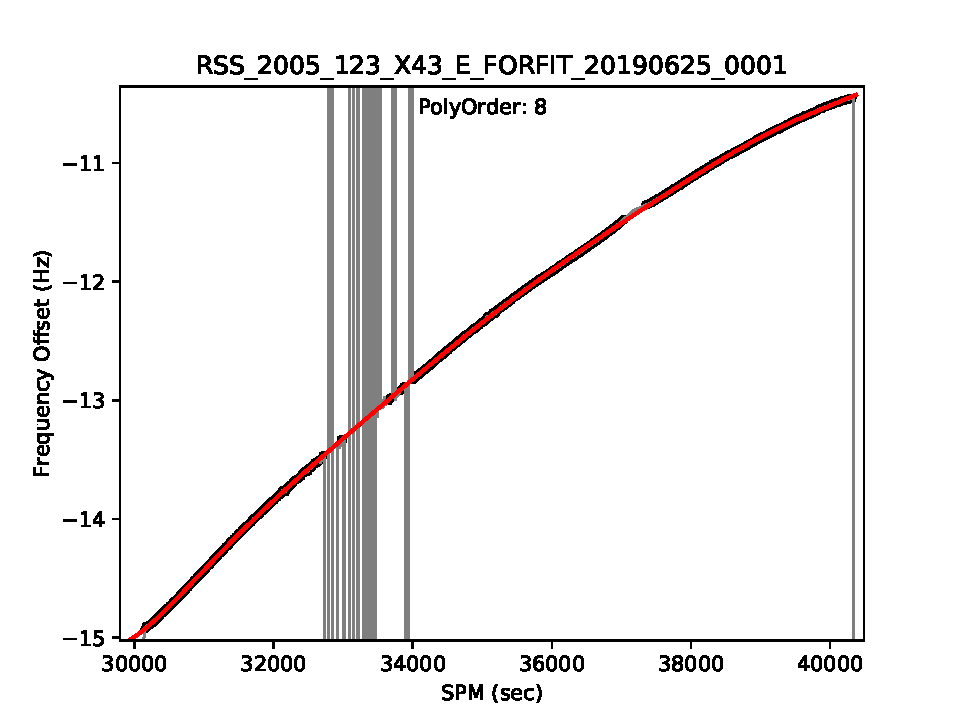
\includegraphics[width=\linewidth]
                    {figs/REV007E_X43_FORFIT_EXAMP.PDF}
                \caption[Example of the frequency offset fit]
                    {Example of the frequency offset fit plot output
                     by the \texttt{FreqOffsetFit} submodule of
                     \texttt{Calibration} step. The total frequency offset
                      $f(t)_{offset}$ is depicted in grey,
                     the $f(t)_{offset}$ used to compute $\hat{f}(t)_{offset}$
                     in black, and the fit $\hat{f}(t)_{offset}$ in red.}
                \label{fig:forfit_examp}
            \end{figure} 
            After computing $\hat{P}_{0}$ from available freespace regions,
            the \texttt{Normalization} class plots power, the power values used
            to compute $\hat{P}_{0}$, and $\hat{P}_{0}$, along with labels
            specifying the fit type, fit order, and information identifying
            the revolution number, direction, wavelength band, DSN station,
            processing date, and processing serial number. \texttt{Normalization}
            saves this plot in a PDF in the subdirectory under \texttt{output}
            corresponding to the current Rev, band, and DSN station. This is
            the same directory as the \texttt{.LBL} and \texttt{.TAB} files
            output by \texttt{rss\_ringoccs} if \texttt{write\_file} is set
            to \texttt{True} (the recommended value). The output PDF is named
            following the same conventions as the \texttt{.LBL} and \texttt{.TAB}
            files, complete with processing date and serial number. We show an
            example of one such output plot in Figure \ref{fig:fspfit_examp} for
            the occultation Rev 007 in the egress direction as observed in the
            X-band from DSN station 43.
    \section{Interactive Mode}
        \label{app:interact}
        When the \texttt{interact} keyword argument is set to
        \texttt{True} when instantiating the \texttt{Calibration} object class,
        the free space power fitting method will enter interactive mode to
        receive user input. After the initial automated fit to the free space
        regions, \texttt{rss\_ringoccs} will plot the results of the fit
        (in the same manner as Figure \ref{fig:fspfit_examp}) in a
        \texttt{matplotlib} window and prompt the user for input in the terminal.
        \begin{figure}[H]
            \centering
            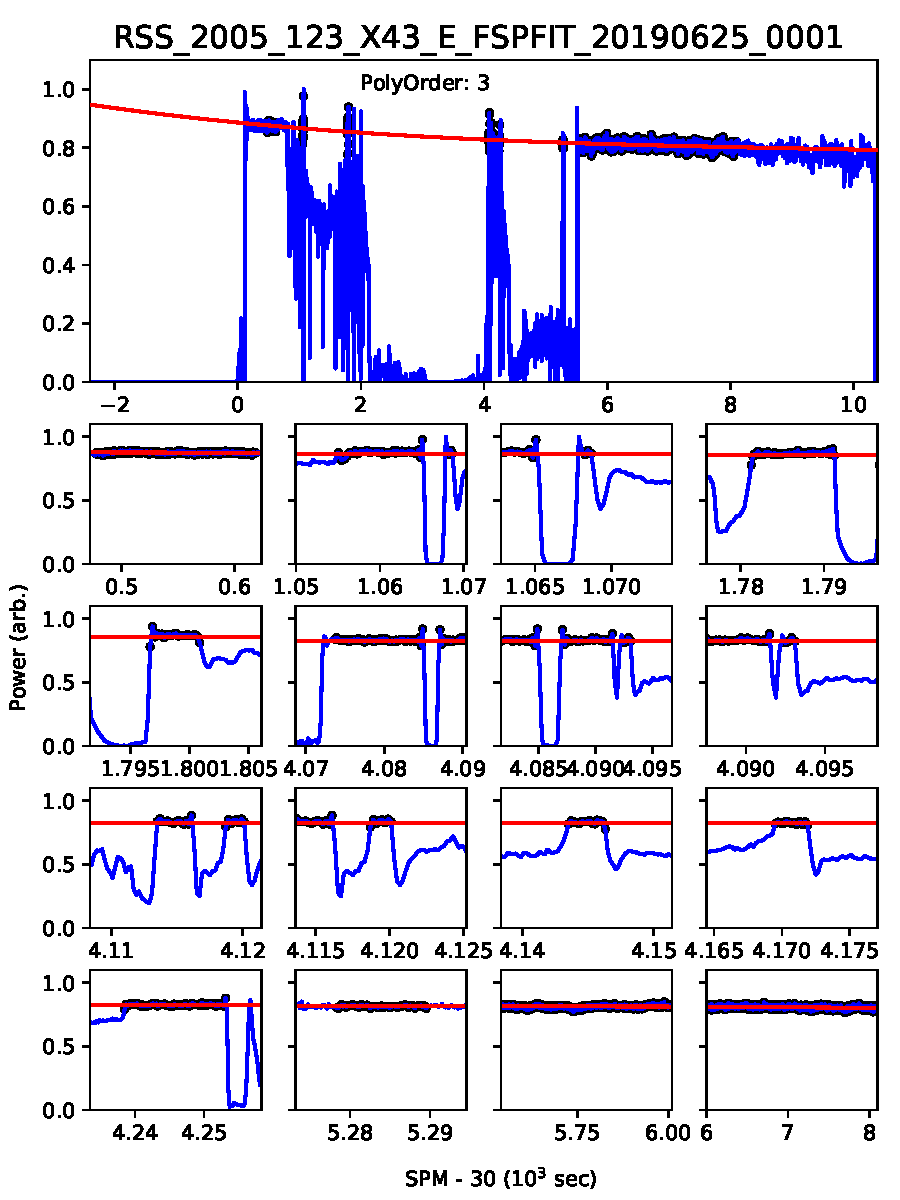
\includegraphics[width=\linewidth]
                {figs/REV007E_X43_FSPFIT_EXAMP.PDF}
            \caption[Example of the free space power fit]
                {Example of the free space power fit plot output by the
                 \texttt{Normalization} submodule of \texttt{Calibration}
                 step. Phase-detrended power is shown in blue, the power used
                 to compute the fit $\hat{P}_0$ to the free space power in
                 black, and the fit $\hat{P}_0$ in red. Top panel is the total
                 power profile. Each subpanel is a closeup of one of the free
                 space regions used in the fit. Subpanels shown in order of
                 time observed (SPM). The number of subpanels will vary
                 depending on the number of freespace regions used in the fit.}
            \label{fig:fspfit_examp}
        \end{figure}
        Here, we explain the input at each prompt and then show an example
        of a single iteration of the interactive mode with possible responses.
        \begin{lstlisting}[%
            language=bash,
            columns=fullflexible,
            basicstyle=\footnotesize\ttfamily,
            literate={~}{$\sim$}{1},
            frame=single,
            escapechar=",
            gobble=12
        ]
            Do you want to continue with this fit? (y/n): n

            Do you want to change the freespace regions? y


            Last used freespace gaps in SPM: 
            [[30477.0, 30618.833698196322],
            [31054.928062871928, 31065.345792559005],
            [31067.770358800513, 31068.930045219375],
            [31780.866566933848, 31791.436274129595],
            [31796.580066071256, 31801.05616095102],
            [34073.68113956013, 34085.4943434775],
            [34086.68935725464, 34091.74708080809],
            [34092.49215200969, 34093.327481330285],
            [34113.3838723948, 34116.39786534125],
            [34118.619852169526, 34120.21853934005],
            [34143.358694145434, 34146.38873649045],
            [34169.41951728726, 34172.05701601253],
            [34238.49233676398, 34253.26244631217],
            [35278.146362236446, 35289.59914281318],
            [35545.59294280804, 36005.16144320606],
            [36005.16144320606, 38092.48430556758]]


            Do you want to revert to the default freespace gaps?  n
            Please input new freespace gaps in SPM and press enter twice: 
            [[30477, 30618],[31055, 31065],[34087, 34091],[34114, 34116],
            [35546, 36005],[36006, 38092]]

            [[30477, 30618],
            [31055, 31065],
            [34087, 34091],
            [34114, 34116],
            [35546, 36005],
            [36006, 38092]]

            What fit type would you like to use? (poly/spline): poly

            What fit order would you like to use?: 3

            Do you want to continue with this fit? (y/n): n
	    \end{lstlisting}
        \begin{enumerate}
            \item Entering \texttt{y} will end interactive mode and accept
                  the current fit. Type \texttt{n} to continue interactive mode
                  and change the fit properties.
            \item \texttt{n} will skip the prompt for new free space regions.
                  \texttt{y} will continue to the prompt for reverting to
                  original free space regions.
            \item \texttt{y} will revert the free space regions to those
                  predicted by the \texttt{Geometry} class and skip the prompt
                  for new free space regions. \texttt{n} will continue to a
                  prompt for new, user-defined free space regions.
            \item User now enters a 2xN list of floats specifying the desired
                  free space regions in SPM (units of seconds). N must be
                  greater than or equal to five in order for the free space
                  fitting to properly select the data in the free space regions.
                  For clarity and verification, the entered freespace regions
                  will be printed to the terminal after the user input is parsed.
            \item Enter the type of fit to use for the freespace power.
                  Two fit types are available, a spline (\texttt{spline}) and a
                  polynomial (\texttt{poly}); however, we highly recommend the
                  polynomial fit.
            \item Enter a whole number between 1 and 9 for polynomial
                  fit or between 1 and 5 for spline fit.
            \item A plot of the new fit made based on the user input will
                  appear in a \texttt{matplotlib} window. The interactive mode
                  will return to the initial prompt about whether to accept the
                  fit or to continue with interactive mode. Return to step 1.
        \end{enumerate}
    \end{appendix}
    % Begin bibliography and glossaries.
    \clearpage
    
    \printglossary[type=\acronymtype]
    \clearpage
    \printglossary[style=longpara]
    \bibliography{biblio}
\end{document}